\documentclass [MS] {UCLAthesis}

\graphicspath{ {figures/} }
\usepackage{microtype}
\usepackage{xcolor}
\definecolor{codegreen}{rgb}{0,0.6,0}
\definecolor{codegray}{rgb}{0.5,0.5,0.5}
\definecolor{codepurple}{rgb}{0.58,0,0.82}
\definecolor{backcolour}{rgb}{0.95,0.95,0.92}

\usepackage{listings}
\lstdefinestyle{mystyle}{
    backgroundcolor=\color{backcolour},   
    commentstyle=\color{codegreen},
    keywordstyle=\color{magenta},
    numberstyle=\tiny\color{codegray},
    stringstyle=\color{codepurple},
    basicstyle=\ttfamily\footnotesize,
    breakatwhitespace=false,         
    breaklines=true,                 
    captionpos=b,                    
    keepspaces=true,                 
    numbers=left,                    
    numbersep=5pt,                  
    showspaces=false,                
    showstringspaces=false,
    showtabs=false,                  
    tabsize=2
}
\lstset{style=mystyle}

%%%%%%%%%%%%%%%%%%%%%%%%%%%%%%%%%%%%%%%%%%%%%%%%%%%%%%%%%%%%%%%%%%%%%%%%
%                                                                      %
%                          PRELIMINARY PAGES                           %
%                                                                      %
%%%%%%%%%%%%%%%%%%%%%%%%%%%%%%%%%%%%%%%%%%%%%%%%%%%%%%%%%%%%%%%%%%%%%%%%

\title          {Visual Tracking with Spiking Neural Networks in an Oculomotor Controller for a Biomimetic Model of the Eye}
\department     {Computer Science}
\author         {Taasin Saquib}
\degreeyear     {2022}

%%%%%%%%%%%%%%%%%%%%%%%%%%%%%%%%%%%%%%%%%%%%%%%%%%%%%%%%%%%%%%%%%%%%%%%%

\chair          {Demetri Terzopoulos}
\member         {Jonathan Kao}
\member         {Sriram Sankararaman}

%%%%%%%%%%%%%%%%%%%%%%%%%%%%%%%%%%%%%%%%%%%%%%%%%%%%%%%%%%%%%%%%%%%%%%%%

\dedication     {\textsl{To Ammu and Abbu, \\
                    for their constant support \\ 
                    and inspiration to be my best self.}}

%%%%%%%%%%%%%%%%%%%%%%%%%%%%%%%%%%%%%%%%%%%%%%%%%%%%%%%%%%%%%%%%%%%%%%%%

\acknowledgments {I would like to express my appreciation to all who made the work of this thesis possible. First, I am grateful for Professor Demetri Terzopoulos' support and guidance in designing this project and providing invaluable feedback. I thank my colleagues in the UCLA Computer Graphics \& Vision Laboratory for their help and interactions. I also acknowledge that the work of this thesis is built upon the work of Dr.~Masaki Nakada who with Arjun Lakshmipathi created the biomimetic eye model and with Honglin Chen created the LiNets and data collection methods for training the oculomotor control system. My thanks to Arjun and Masaki for their guidance and assistance.}

%%%%%%%%%%%%%%%%%%%%%%%%%%%%%%%%%%%%%%%%%%%%%%%%%%%%%%%%%%%%%%%%%%%%%%%%

\vitaitem   {2017}
                {Full Stack Software Engineering Intern, Project Looma, 
                Village Tech Solutions, Palo Alto, California.}
\vitaitem   {2018}
                {Software Engineering Intern, Device Drivers, 
                Nvidia, Santa Clara, California.}
\vitaitem   {2019}
                {Software Engineering Intern, Device Drivers, 
                Nvidia, Santa Clara, California.}
\vitaitem   {2020}
                {B.S.~(Computer Science and Engineering),
                University of California, Los Angeles.}
\vitaitem   {2020}
                {Software Engineering Intern, Traffic Engineering, 
                Splunk, San Jose, California.}
\vitaitem   {2020--present}
                {Teaching Assistant, Computer Science Department, UCLA.\\ 
                Taught CS 31 (Introduction to Computer Science I) under the direction of Professor David Smallberg (Fall 2020).\\
                Taught CS 32 (Introduction to Computer Science II) under the direction of Professor David Smallberg (Winter 2021, Spring 2021).\\ 
                Taught CS M51A (Logic Design of Digital Systems) under the direction of Professor Richard Korf (Fall 2021).}
\vitaitem   {2021--present}
                {Graduate Researcher, UCLA Computer Graphics \& Vision Laboratory, 
                Computer Science Department, University of California, Los Angeles.}

%%%%%%%%%%%%%%%%%%%%%%%%%%%%%%%%%%%%%%%%%%%%%%%%%%%%%%%%%%%%%%%%%%%%%%%%

\abstract {
Spiking neural networks (SNNs) are comprised of artificial neurons that, like their biological counterparts, communicate via electrical spikes. SNNs have been hailed as the next wave of deep learning as they promise low latency and low power consumption when run on neuromorphic hardware. Current deep neural network models for computer vision often require power-hungry GPUs to train and run, making them great candidates to replace with SNNs. In this thesis, we develop and train an SNN-based foveation deep neural network that enables a biomechanical model of the human eye to track a moving visual target. Inspired by the ON and OFF bipolar cells of the retina, we use event-based data flow in the SNN to direct the necessary extraocular muscle-driven eye movements. While many SNNs are conversions of trained deep neural network architectures, we train our SNN models from scratch using modified deep learning techniques. Classification tasks are straightforward to implement with SNNs and have received the most research attention, but visual tracking is a regression task. We use surrogate gradients and introduce a linear layer to convert membrane voltages from the final spiking layer into the desired outputs. Our SNN foveation network is noisier than the previously used deep neural network, but it enhances the biomimetic properties of our virtual eye model and enables it to perform reliable visual tracking.
}

%%%%%%%%%%%%%%%%%%%%%%%%%%%%%%%%%%%%%%%%%%%%%%%%%%%%%%%%%%%%%%%%%%%%%%%%

\begin {document}
\makeintropages

%%%%%%%%%%%%%%%%%%%%%%%%%%%%%%%%%%%%%%%%%%%%%%%%%%%%%%%%%%%%%%%%%%%%%%

\chapter{Introduction}

The human visual system is an astounding computational machine. Photons impact the retina and, through neural processing, enable the visual cortex to perform multiple visual tasks quickly, with high precision, and using very little energy. Artificial neural network (ANN) based computer vision algorithms have come far in recreating the performance of the visual cortex in terms of accuracy, but they employ power-hungry GPUs that lag behind the power and low-latency performance of the human brain.

Spiking neural networks (SNNs) \citep{snn_survey}, comprised of interconnected spiking neurons that, like their biological counterparts, communicate via electrical spikes, are hailed as the ``third wave of deep learning.'' This is because they feature a more biologically-inspired neuronal model that consumes much less power than the standard artificial neurons now commonly in use. Many traditional AI tasks can be achieved with SNNs implemented using the appropriate hardware, which is referred to as ``neuromorphic'' and currently takes the form of what are known as neuromorphic chips \citep{snn_hw_survey}.

\begin{figure}
\centering
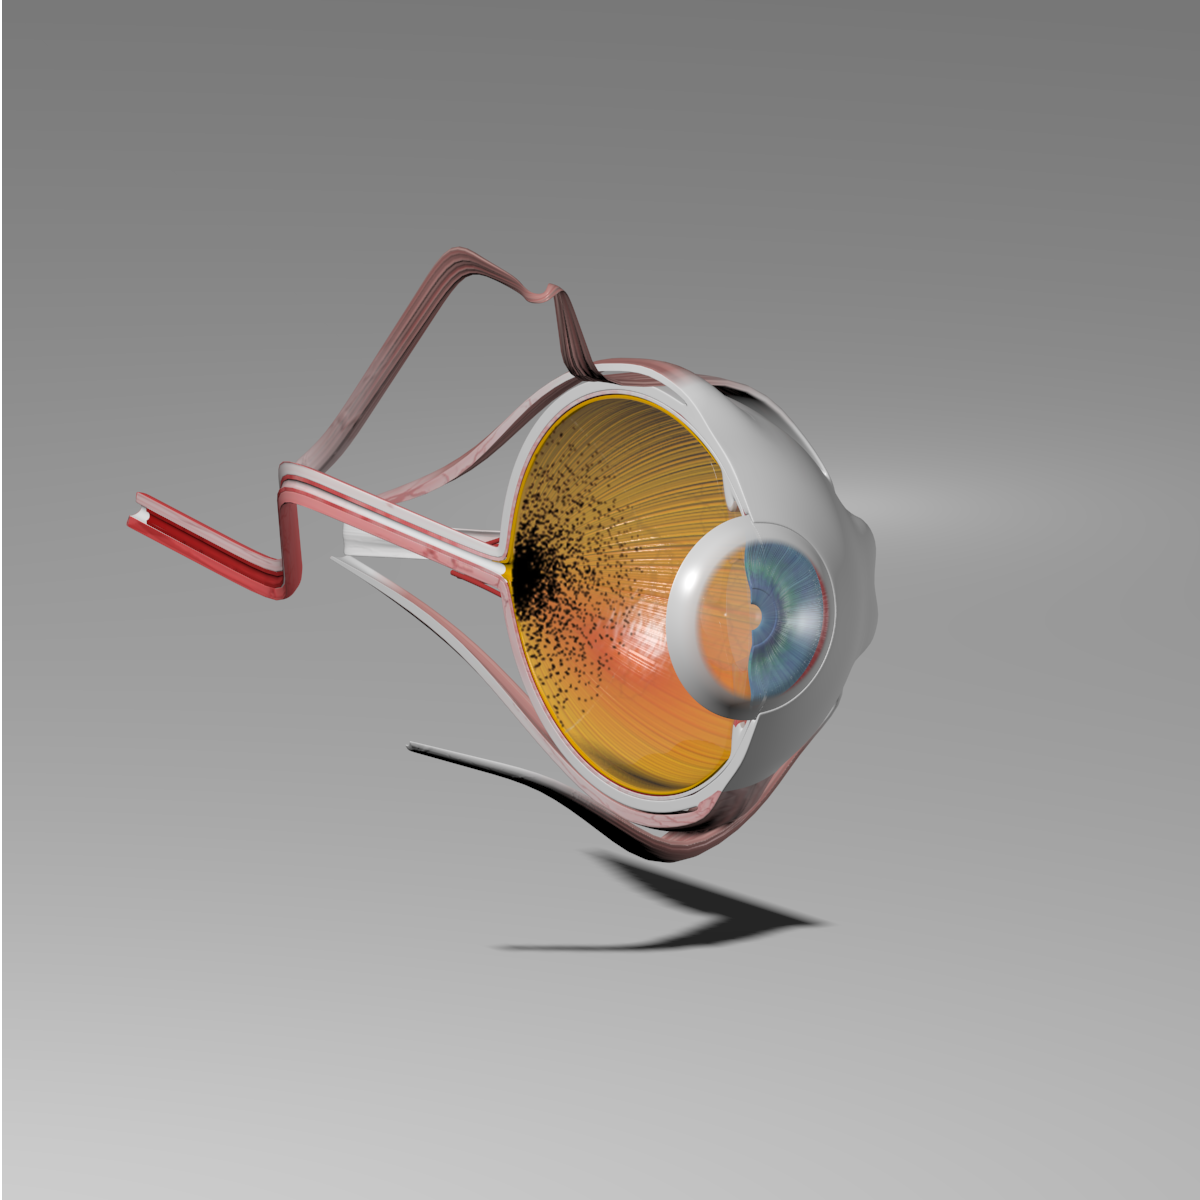
\includegraphics[width=0.545\linewidth,trim={0 60mm 10mm 60mm},clip]{disected_eye_final}
\caption[The biomimetic eye model]{(Cross section of a detailed geometric model of the left eye. The black dots on the retina indicate the positions of retinal photoreceptors.
Image from \citep{Arjun}.}
\label{fig:eye}
\end{figure}

This thesis explores the design and training of an SNN in a computer vision task. Our work builds upon that of \citet{Arjun_thesis} and \citet{Arjun} who developed a biomechanical model of the human eye with a comprehensive set of ocular organs, as well as a neuromuscular oculomotor control system for this realistic simulation model.\footnote{This model of the eye was a vast improvement over a simpler eye model created as part of the biomechanical human musculoskeletal model developed by \citet{Masaki}.} 
Of specific interest in this thesis is one of the neural networks within the perception subsystem of the oculomotor controller. The network, described in greater detail in the paper by \citet{Masaki_linet}, was referred to as the foveation LiNet or locally-connected irregular network. While the biomimetic eye model can synthesize realistic eye motion, the ``neurons'' comprising the artificial neural networks in its oculomotor controller are only high-level abstractions of biological neurons. This thesis aims for additional biological realism through the use of spiking neurons interconnected to form SNNs. To this end, we explore how to encode our floating-point signals into spike trains, which is the job of photoreceptors in the mammalian retina. It remains unclear whether the visual system uses rate or latency encoding \citep{encoding_retina}, both of which we consider in our work. In addition, we train our SNNs on event-based data, which emulates the ON-OFF bipolar cells of the retina. Our effort is aimed at enhancing the biological realism of the eye model.

%********************************************************************%

\section{Thesis Contributions}

More precisely, the contributions of the thesis are as follows:
\begin{enumerate}
    \item We devise a novel foveation LiNet, based on SNNs, which we call the SLiNet, to enable the oculomotor control of our biomimetic eye model. Unlike the previous network for this model \citep{Arjun}, ours yields an event-based sensory system that responds only to changes in the light intensities sensed by the eye rather than to the absolute intensity values themselves. This is more biologically accurate and creates a sparser input to the oculomotor controller.
    \item To accomplish the above, we design an SNN architecture than can solve a regression task, which is more difficult than the classification tasks to which SNNs have typically been applied.
  \item Unlike the typical deployment of previous SNNs, we train our SliNet from scratch. To this end,
  \begin{itemize}
    \item we consider rate and latency encoding, the two most commonly used encoding methods, and find the best encoding parameters for each method, and
    \item we use a surrogate gradient to solve the ``dead neuron problem'' and enable the use of standard deep learning optimization techniques.
  \end{itemize}
  \item The work of \citet{Arjun} and the MS thesis of \citet{Arjun_thesis} developed the biomimetic eye model and demonstrated its biological accuracy by testing it on different types of eye movements (saccade, fixation, and smooth pursuit). We use the same experimental regimen to test our SLiNet's performance on both conventional and event-based data.
\end{enumerate}

%********************************************************************%

\section{Thesis Overview}

The remainder of this thesis is organized as follows:

Chapter 2 surveys the relevant literature related to the use of SNNs in computer vision.

Chapter 3 prescribes the visual tracking task of interest and presents the details of the biomimetic eye model with which we work.

Chapter 4 compares artificial neurons to spiking neurons and explains how SNNs operate, which includes exploring how to encode our inputs and interpret the output spike trains.

Chapter 5 describes the architecture of our SNN as well as the associated training techniques.

Chapter 6 reports our results and compares our SNN performance to that of the previous LiNet architecture.

Chapter 7 presents our conclusions and suggests promising avenues for future work.

%%%%%%%%%%%%%%%%%%%%%%%%%%%%%%%%%%%%%%%%%%%%%%%%%%%%%%%%%%%%%%%%%%%%%%

\chapter{Related Work}

In this chapter, we review relevant prior research related to SNNs.

%********************************************************************%

\section{Neuromorphic Hardware}

Currently, graphics processing units (GPUs), the workhorses of deep learning based artificial intelligence using ANNs, are optimized for highly parallelized multiply-and-accumulate (MAC) operations on floating-point numbers and consume large amounts of power. By contrast, neuromorphic chips take advantage of the fact that spiking activation functions only output 1's and 0's and hence operate with low power consumption. They are also optimized for the asynchronous nature of spikes and can run new types of learning algorithms. 

Several major corporations are investing in the design and manufacture of neuromorphic chips. Intel's Loihi \citep{8259423} is on its third generation, and IBM, Samsung, and other large companies are betting on the future of this sector. However, because this hardware is still difficult to acquire, we run our SNNs on a GPU.

% neuromorphic cochlea, DVS, etc.
In addition to neuromorphic chips, neuromorphic sensors are also under development. Vision has been the sensory modality to receive the most attention, and dynamic vision sensor (DVS) cameras, or ``silicon retinas,'' are slowly entering more and more systems. Instead of capturing data one frame at a time, these cameras simply record if pixels in their sensory arrays have gotten brighter or darker. If such a change occurs at any pixel, the camera outputs a timestamped ``event.'' The DAVIS sensor \citep{davis_dvs} is one example of a DVS camera. New spiking datasets are being created with DVS sensors, as shown in Figure~\ref{fig:dvs_ex}. 

% images of event-based data
\begin{figure}
     \centering
     \begin{subfigure}{0.41\textwidth}
         \centering
         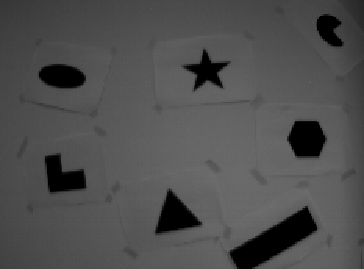
\includegraphics[width=\textwidth]{dvs1}
         \caption{}
         \label{fig:dvs1}
     \end{subfigure}
     \hfill
     \begin{subfigure}{0.4\textwidth}
         \centering
         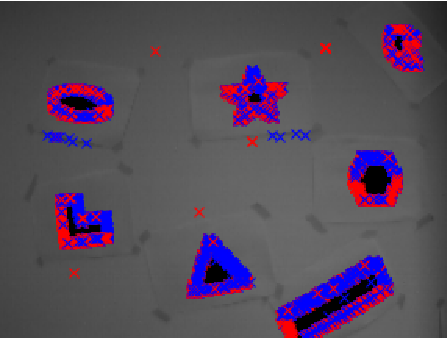
\includegraphics[width=\textwidth]{dvs2}
         \caption{}
         \label{fig:dvs2}
     \end{subfigure}
    \caption[Example data recorded from a DVS camera]{This dataset records a DVS camera moving around a collection of shapes. The camera has moved slightly between the frames in (a) and (b). The resulting changes in pixel intensities are shown in (b), where pixels that have brightened are marked in red while those that have darkened are marked in blue. Images from \citep{spiking_shapes}.}
    \label{fig:dvs_ex}
\end{figure}

% Another popular sensor is the "silicon cochlea." Inspired by the real cochlea, there are 64 channels that produce events in response to sound of different frequencies \citep{silicon_cochlea}.

%********************************************************************%

\section{Converting Artificial Neural Networks into SNNs}

Many researchers want the benefits of SNNs, but they also prefer to avoid training them. This has prompted research into converting trained artificial neural networks (ANNs) into SNNs. The main advantage of this approach is that one need not work around the non-differentiability of the spiking activation function and can effectively train a model with standard deep learning techniques.

\citet{convert_no_bias} are credited with developing early conversion techniques for fully connected networks. Now, almost any existing neural network layer can be converted into a spiking equivalent, including convolution and softmax layers \citep{convert_with_bias}. These converted models may have slightly higher error rates, but they can offer about a 2x reduction in the number of operations when compared to the original ANNs.

In this thesis, however, we aim to train SNNs directly rather than convert them from trained ANNs. We take this approach not just because converted SNNs typically require neurons to have high spiking frequencies, which results in the consumption of more power, thereby undermining the benefits of using SNNs in the first place. More importantly, we aim to explore event-based data in a biologically plausible setting. Converted models are typically trained on data with events calculated after the fact and they perform poorly when fed more realistic spiking data from a DVS sensor.

% Performance of these two learning techniques?
We also open the door to the use of more biologically-inspired, unsupervised learning techniques to train our model in the future. In particular, spike timing dependent plasticity (STDP), or Hebbian learning, has shown great promise \citep{KHERADPISHEH201856}. Winner-take-all (WTA) circuits that make use of inhibition are also of much interest.

%********************************************************************%

\section{SNNs and Computer Vision}

Traditional computer vision tasks are being addressed with SNNs. MNIST handwritten digit classification remains a popular benchmark \citep{stdp}, but SNNs also perform well on more complex datasets such as ImageNet. \citet{10.3389/fnins.2019.00095} develop an SNN based on VGGNet and achieve a top-5 error rate of 30.04, whereas the state-of-the-art ANN achieves a top-5 error rate of 29.48. Other complex models such as ResNet have been trained to work directly with spiking input from a DVS camera \citep{resnet_events}.

% explain classification in SNNs and why regression is hard
Most computer vision research with SNNs to date has chosen to work with classification problems. It is often stated in the literature that SNNs are easier to apply to classification problems than to regression problems. This is due to the fact that there is consensus on how to interpret spike trains so as to classify an input, but there are many choices in how to interpret spike trains to represent continuous quantities. The only published work on regressions with SNNs is by \citet{regression_steering} and \citet{spiking_yolo}. However, their SNN models were converted from a trained ANN. We train our SNN from scratch and offer an alternative approach to creating an output layer for a regression problem.

Our eye model has a biomimetic, nonuniform photoreceptor distribution, whereas the pixels in images from datasets such as MNIST and CIFAR-10 are conventionally arranged in structured arrays. Permutation invariant MNIST, or PI-MNIST \citep{le2015simple}, is an interesting dataset that alters the arrangement of pixels so that standard convolutional layers cannot be used to classify digits and serves as the only benchmark that remotely resembles the unstructured input of the retinal model of interest in this thesis.

%%%%%%%%%%%%%%%%%%%%%%%%%%%%%%%%%%%%%%%%%%%%%%%%%%%%%%%%%%%%%%%%%%%%%%

\chapter{The Task}

Our goal is to create an SNN that, when properly trained, enables the biomimetic eye model of \citet{Arjun} to track a 3D object through space. The visual target of choice is a white ball that moves against a background whose intensity varies in different shades of grey due to changing illumination. The eye model's oculomotor controller has four main parts, one of which we implement as an SNN. We test our implementation by checking that our modified controller performs certain movements with biological accuracy and that it can successfully track the target. In this section, we provide more details about the eye model and its oculomotor controller and focus on the retina and the foveation deep neural network (DNN) that we replace with an SNN.

%********************************************************************%

\section{Retina}

Like a biological retina, our virtual retina is situated at the back of the eye and has photoreceptors that sense light from the scene. Each photoreceptor collects a red, green, and blue color value. The $N$ photoreceptors are nonuniformly distributed according to a noisy log-polar distribution
\begin{equation}
d_k = e^{\rho_j} 
    \begin{bmatrix} 
        \cos( \alpha_i) \\ 
        \sin( \alpha_i) 
    \end{bmatrix}
    +
    \begin{bmatrix} 
        \mathcal{N}(\mu, \sigma^2) \\ 
        \mathcal{N}(\mu, \sigma^2)
    \end{bmatrix},
    \text{ for }
    1 \leq k \leq \text{N},
    \label{eq:log-polar}
\end{equation}
where $\mathcal N(\mu, \sigma^2)$ denotes IID-sampled Gaussian noise of mean $\mu$ and variance $\sigma^2$. This distribution places most of the photoreceptors near the center of the retina, forming a foveal region that supports high acuity central vision, with progressively diminishing visual resolution towards the retinal periphery.

% cite papers about actual eye structure

A visualization of the photoreceptor distribution on the retina is shown in Figure~\ref{fig:task_log_polar_retina}. Here, we have chosen $N=\text{14,400}$ photoreceptors in (\ref{eq:log-polar}), incrementing $\rho_j$ and $\alpha_i$ in steps of 1 such that $0 \leq \rho_j \leq 40$ and $0 \leq \alpha_i \leq 360$. The additive Gaussian noise distribution has mean $\mu = 0$ and variance $\sigma^2 = 0.0025$.  Using fewer photoreceptors speeds up simulation and training, but the number of photoreceptors can be scaled up to match human retinas (which have about 6 million cone photoreceptors supporting normal color vision and about 120 million rod photoreceptors supporting monochrome low-light vision \citep{rodsAndCones}).

\begin{figure}
    \centering
    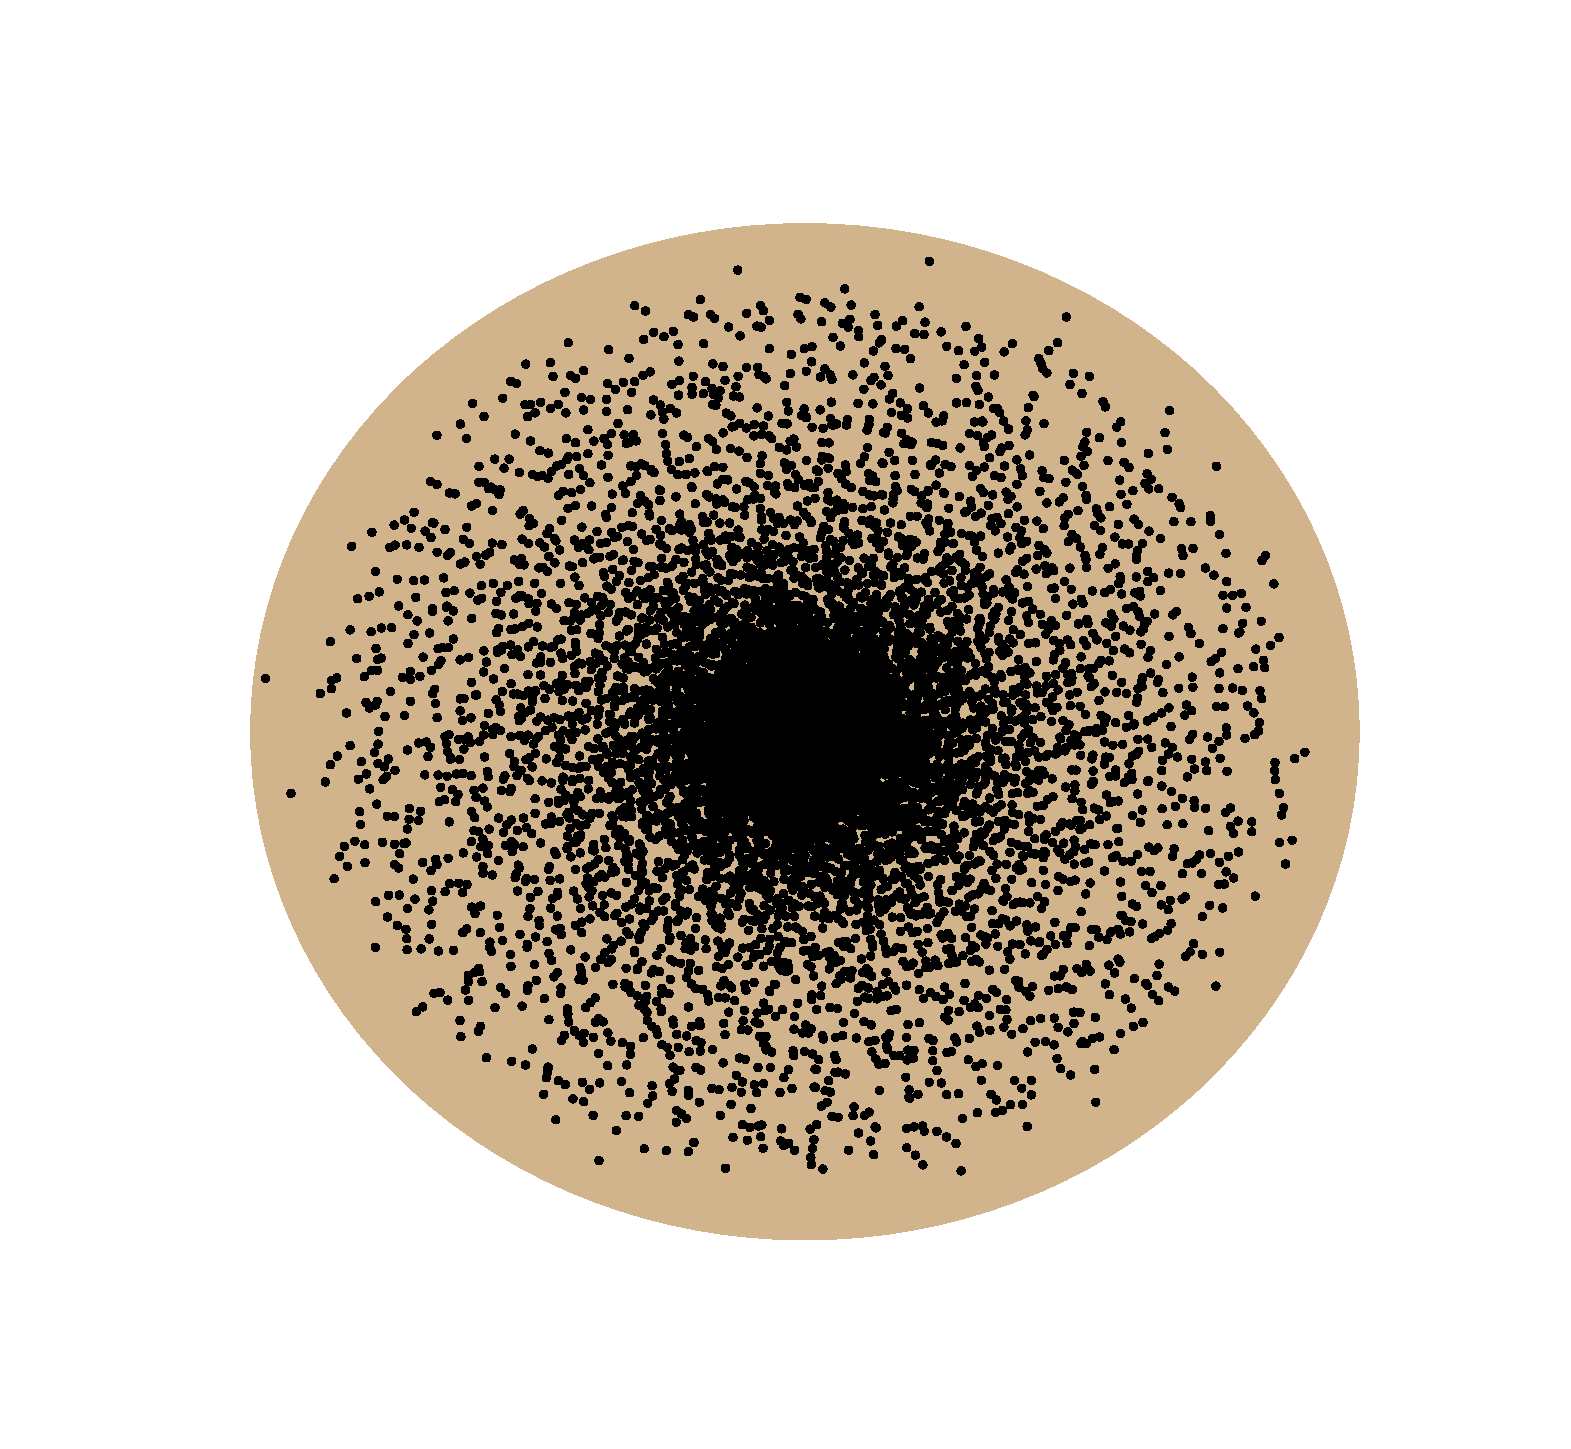
\includegraphics[width=0.6\textwidth,height=0.605\textwidth]{retina_log_polar}
    \caption[Photoreceptor distribution on the retina]{The photoreceptors on the retina are arranged according to a 2D noisy log-polar distribution, which is mapped to the hemispherical fundus of the eyeball.}
    \label{fig:task_log_polar_retina}
\end{figure}

To compute the amount of light registered by each photoreceptor, in accordance with the ray tracing procedure that is well-known in computer graphics \citep{ray_tracing}, rays are cast from the positions of photoreceptors on the retinal surface, refracted through the deformable lens of the eye, through the pupil, again diffracted through the cornea, and out into the 3D environment to recursively intersect with environmental objects in the scene and sample the lightsources (Figure~\ref{fig:raytracing}). The computed color values returned from the recursion determine the irradiance at each photoreceptor, thus resulting in 14,400 RGB values. We stack the RGB values of each photoreceptor into a $3N=\text{43,200}$-dimensional vector, which \citet{Masaki} refer to as the optic nerve vector (ONV).

\begin{figure}
\centering
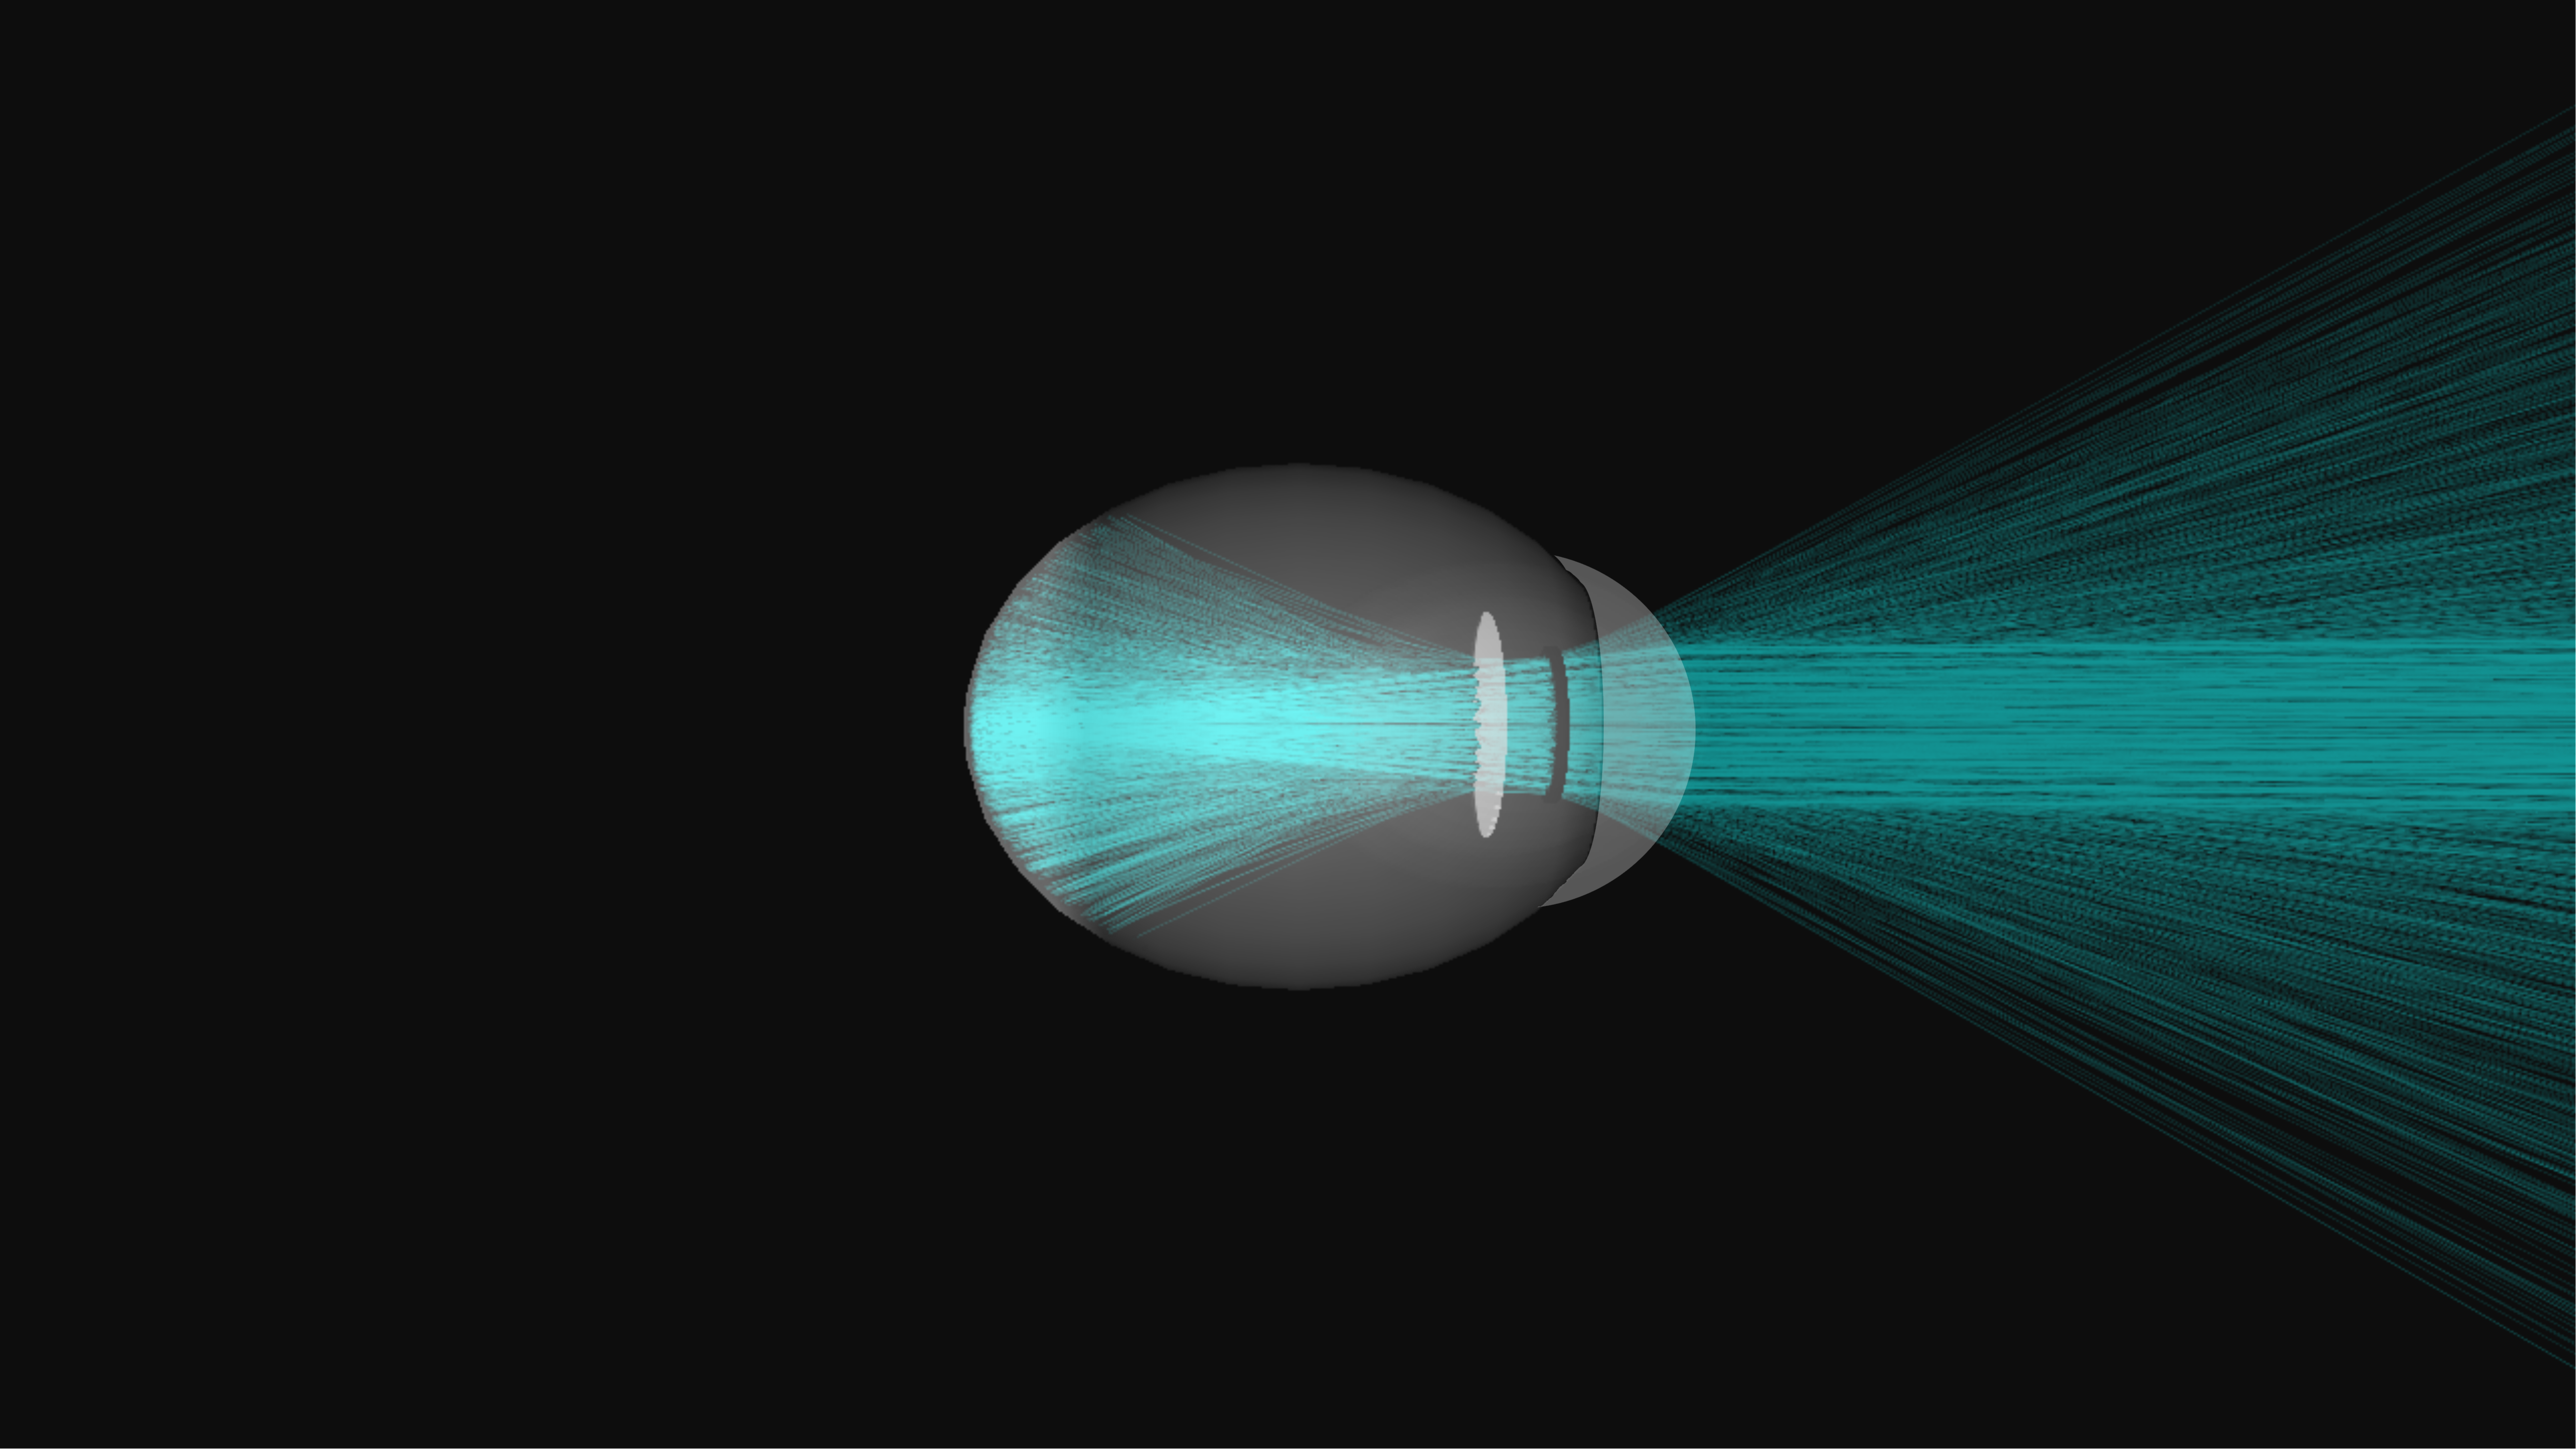
\includegraphics[width=0.44\linewidth,height=0.40\linewidth,trim={300mm 30mm 0 30mm},clip]{tracemodeloverlaybiggercornea}
\caption[Ray tracing in the eye model]{Rays
cast from the positions of the photoreceptors through the
finite-aperture pupil and out into the scene to compute the irradiance
responses of the photoreceptors according to the ray tracing process. Image from \citep{Arjun}.}
\label{fig:raytracing}
\end{figure}

\section{LiNets}
\label{sec:LiNets}

The next step is one of visual processing analogous to that taking place in the visual cortex of the brain. Convolutional neural networks (CNNs), which abstractly model the connectivity of neurons in the visual cortex, have enabled much progress in computer vision. In CNNs, each neuron is connected only to its neighboring neurons in the previous layer, thereby forming what are known as ``receptive fields''. The stylized, highly regular receptive fields of conventional CNNs exploit the fact that ordinary images are structured as rectangular arrays of pixels. 

By contrast, the biomimetic photoreceptor distribution on the retina in our eye model is an irregular, foveated distribution, and the ONV exiting the retina is simply a vector of photoreceptor responses rather than a 2D pixel-array image. Therefore, the ONV is incompatible with CNNs. Consequently, \citet{Arjun} generalized CNNs by introducing locally-connected irregular networks or ``LiNets'' \citep{Masaki_linet}. The LiNet architecture is illustrated in Figure~\ref{fig:linet_rgb}. Neurons have associated positions within the visual field. According to these positions, each neuron is connected only to the $n$ nearest neurons in the previous layer, thus forming overlapping circular receptive fields at the retinal level, which are shown as white circles in the figure. The number of neurons in successive layers is scaled down by a factor $f$. 

Like CNNs, LiNets consume far less memory than comparably-sized fully-connected networks, thus accommodating retinas with large numbers of photoreceptors. However, unlike CNNs, the receptive fields of neurons within a given layer do not share weights (i.e., they are not convolutional), so the memory requirements of LiNets are generally greater than those of CNNs.

% \begin{figure}
%     \centering
%     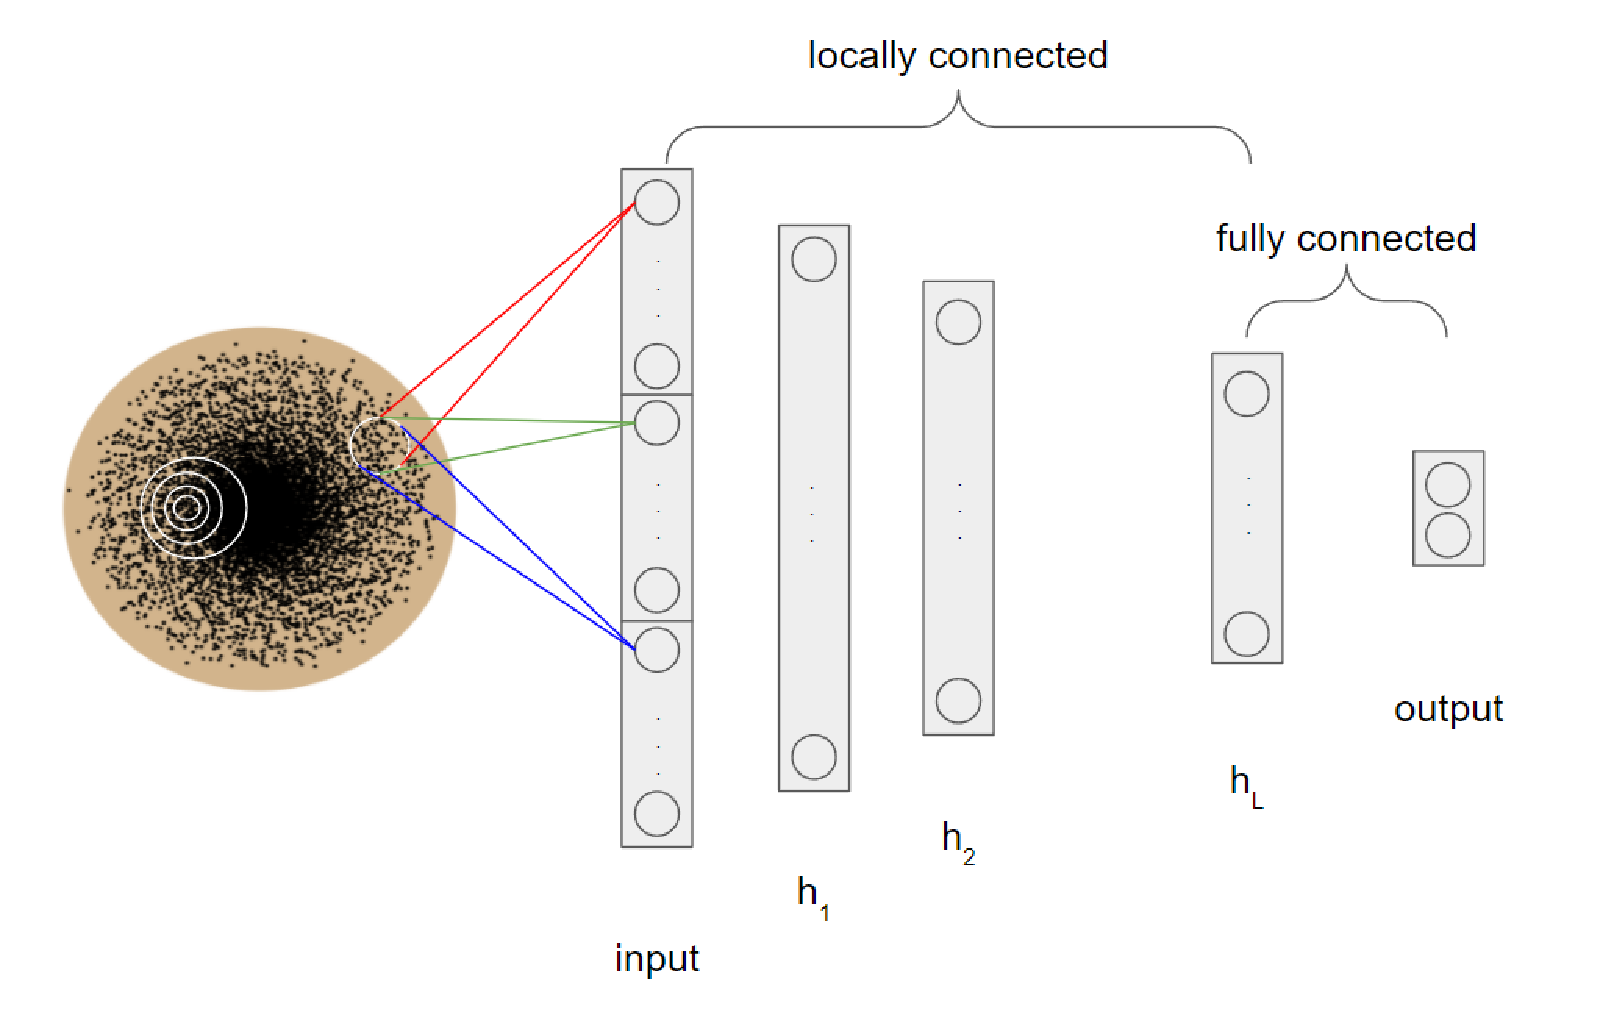
\includegraphics[width=\textwidth]{linet_summary}
%     \caption[LiNet architecture summary]{The LiNet architecture. We have a 14,400 photoreceptor retina with red, blue and green channels stacked on top of each other to create the ONV. Each neuron then processes the K nearest red, blue, or green inputs to it. Neurons at the first layer combine input from a handful of photoreceptors. Neurons in consecutive layers combine the fields of view from previous layers to slowly get closer to seeing the full scene.}
%     \label{fig:linet_rgb}
% \end{figure}

\begin{figure}
    \centering
    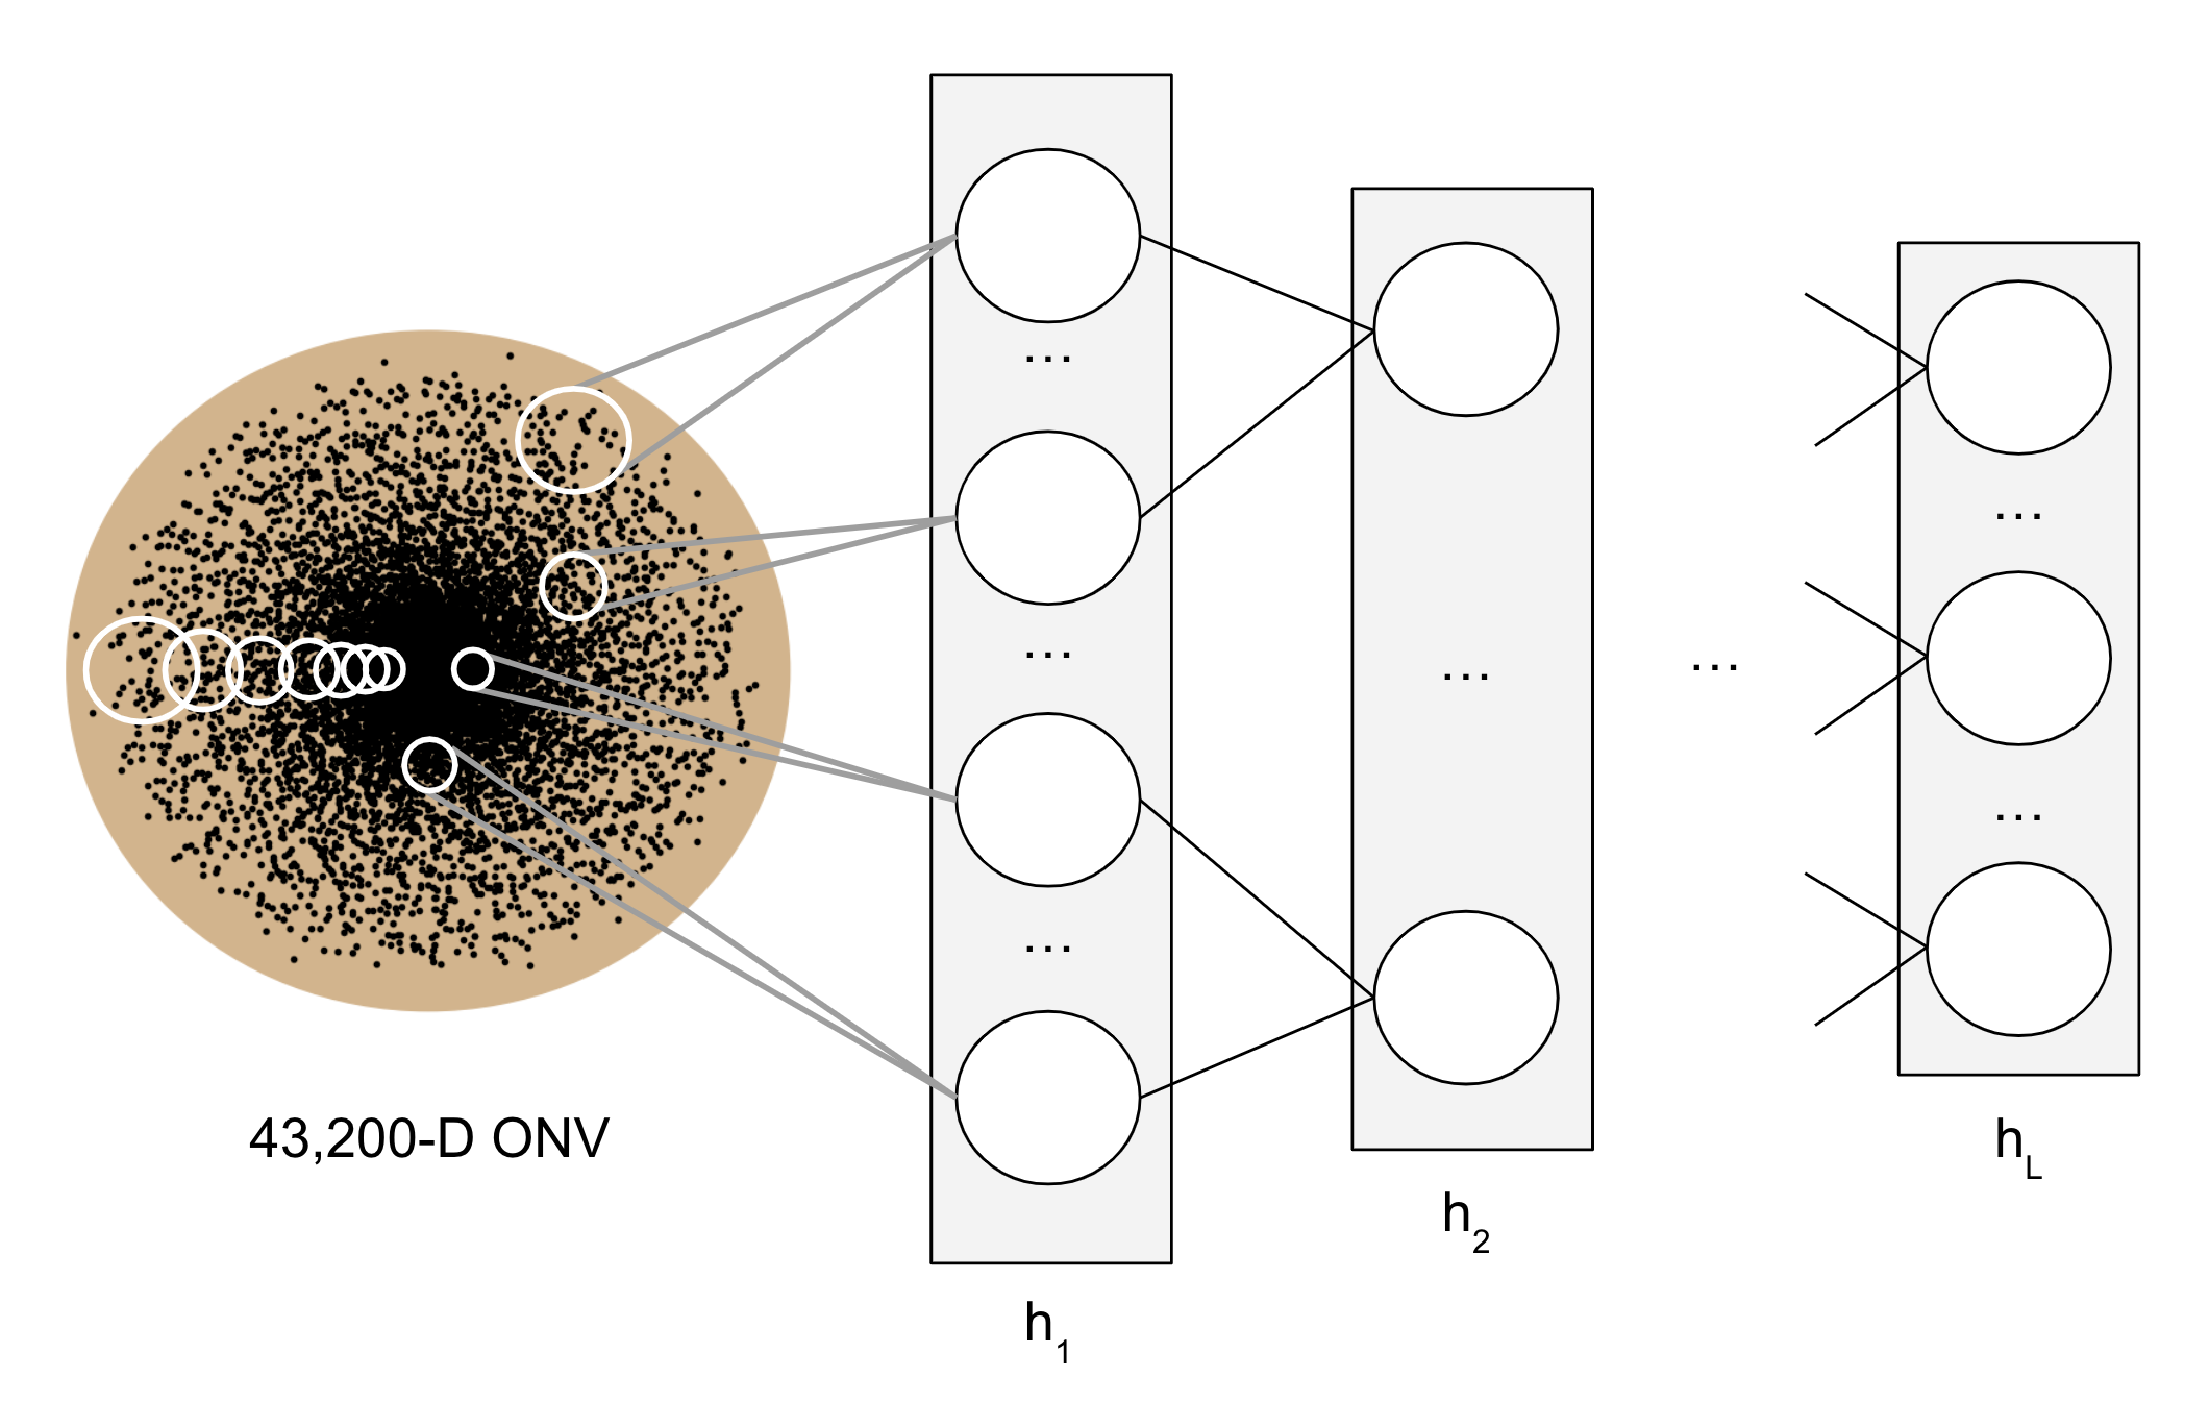
\includegraphics[width=0.8\textwidth]{linet_summary2}
    \caption[LiNet architecture]{The LiNet architecture. We have a 14,400 photoreceptor retina that creates the input ONV. Neurons at the first layer combine input from a handful of photoreceptors. Because photoreceptors are more densely packed towards the center of the retina, receptive fields get larger towards the periphery. Neurons in consecutive layers combine the fields of view from previous layers to slowly get closer to seeing the full scene.}
    \label{fig:linet_rgb}
\end{figure}

%********************************************************************%

\section{Oculomotor Control}

In addition to the retina, lens, pupil, and cornea, the biomimetic eye model includes the 6 extraocular (EO) contractile muscles. The cornea and deformable lens focus visual targets onto the retina while the EO muscles drive the eye movements necessary to foveate and track visual targets in motion. Each muscle requires a time-varying motor activation signal that stimulates it to contract. An oculomotor controller is responsible for producing the muscle activation signals that drive the eye movements needed to accomplish the visual task of interest.

Additional details about the eye model and its oculomotor control system are provided in Appendix~\ref{appendix:eye}. The latter comprises a sensory subsystem and a motor subsystem, as shown in Figure~\ref{fig:eye_controller_summary}. The ONV is input to the foveation DNN, which is implemented as a LiNet. This foveation LiNet outputs 2 values, $\Delta\theta$ and $\Delta\phi$, that represent a desired change in the horizontal and vertical gaze angles relative to the eye's current gaze direction. Figure~\ref{fig:ball_movement} presents an example of how we encode the motion of a white ball visual target with these two gaze angles. The neuromuscular DNN is then fed the outputs of the foveation LiNet and outputs an activation signal for each of the 6 EO muscles to induce the required eye movement.

\begin{figure}
     \centering
     \begin{subfigure}{0.48\textwidth}
         \centering
         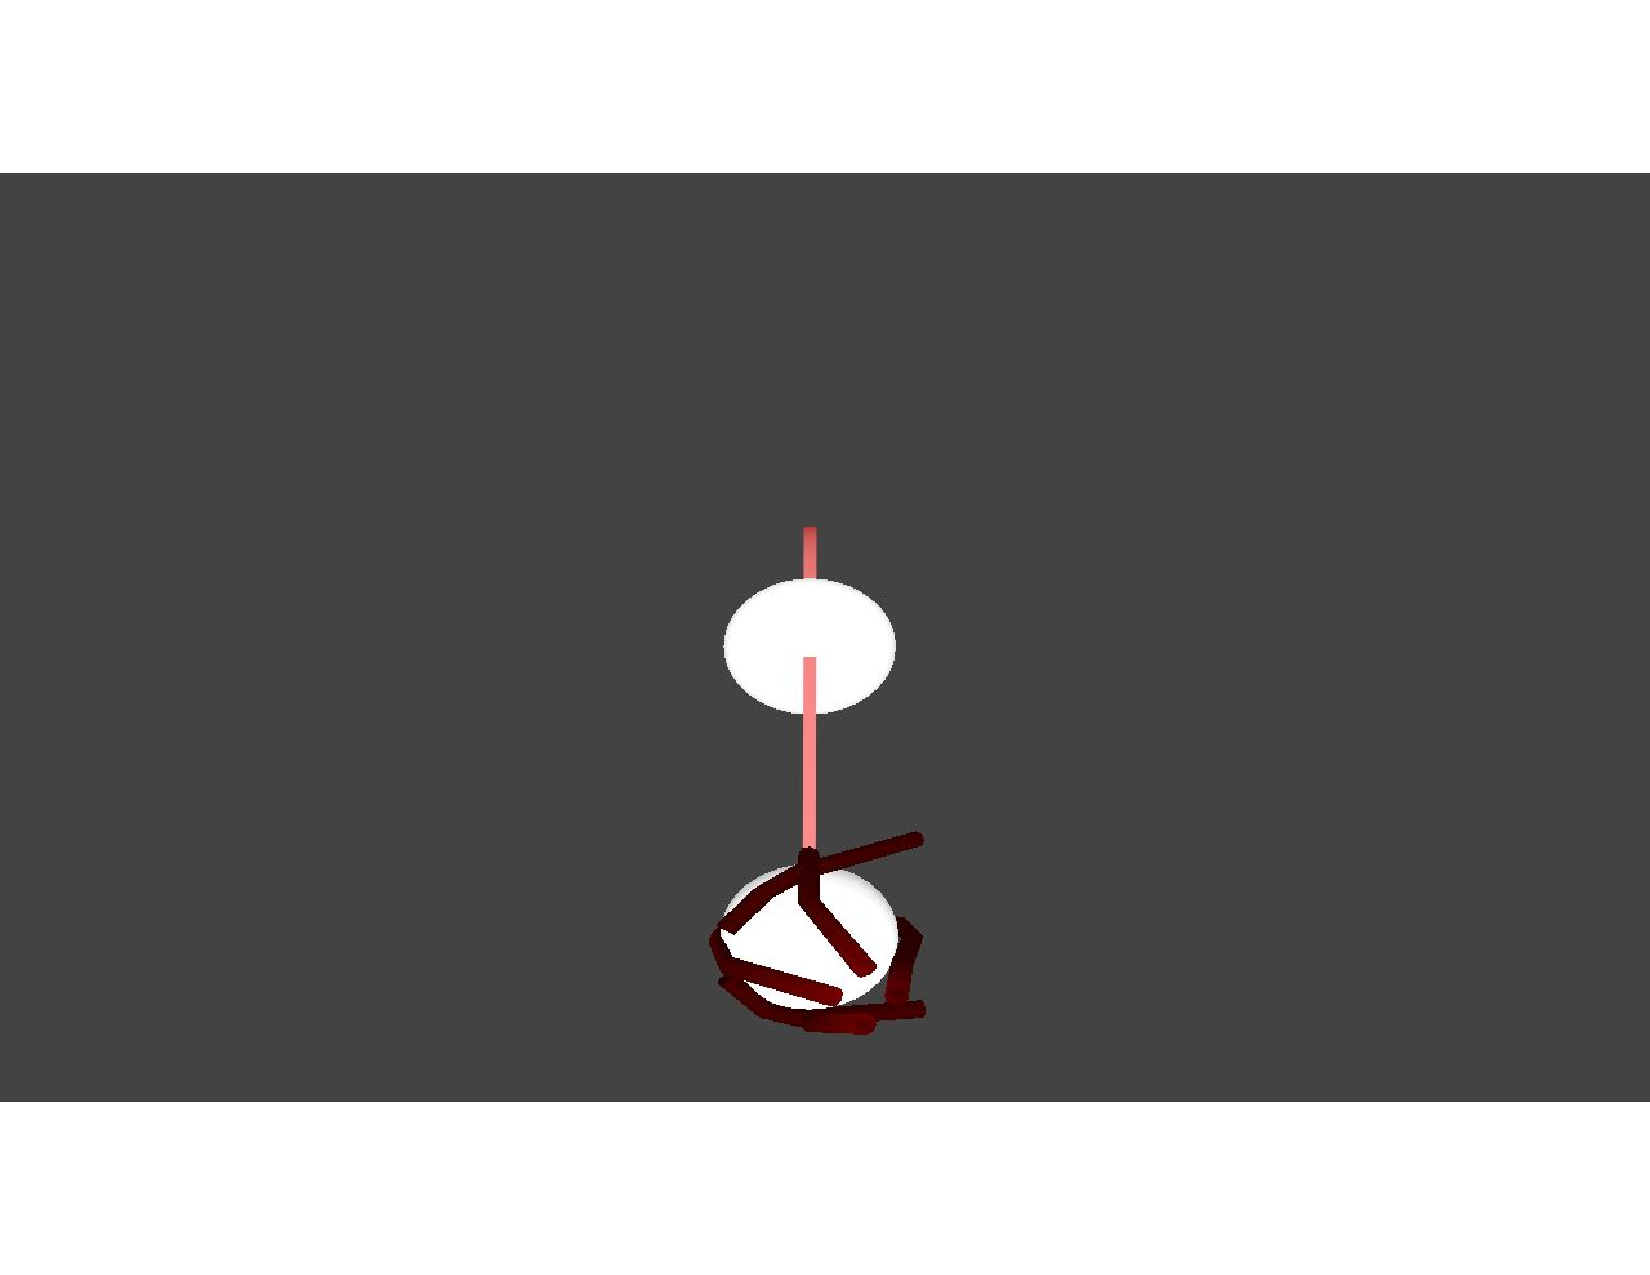
\includegraphics[width=\textwidth]{image000028}
         \caption{}
         \label{fig:ball_pos1}
     \end{subfigure}
     \hfill
     \begin{subfigure}{0.48\textwidth}
         \centering
         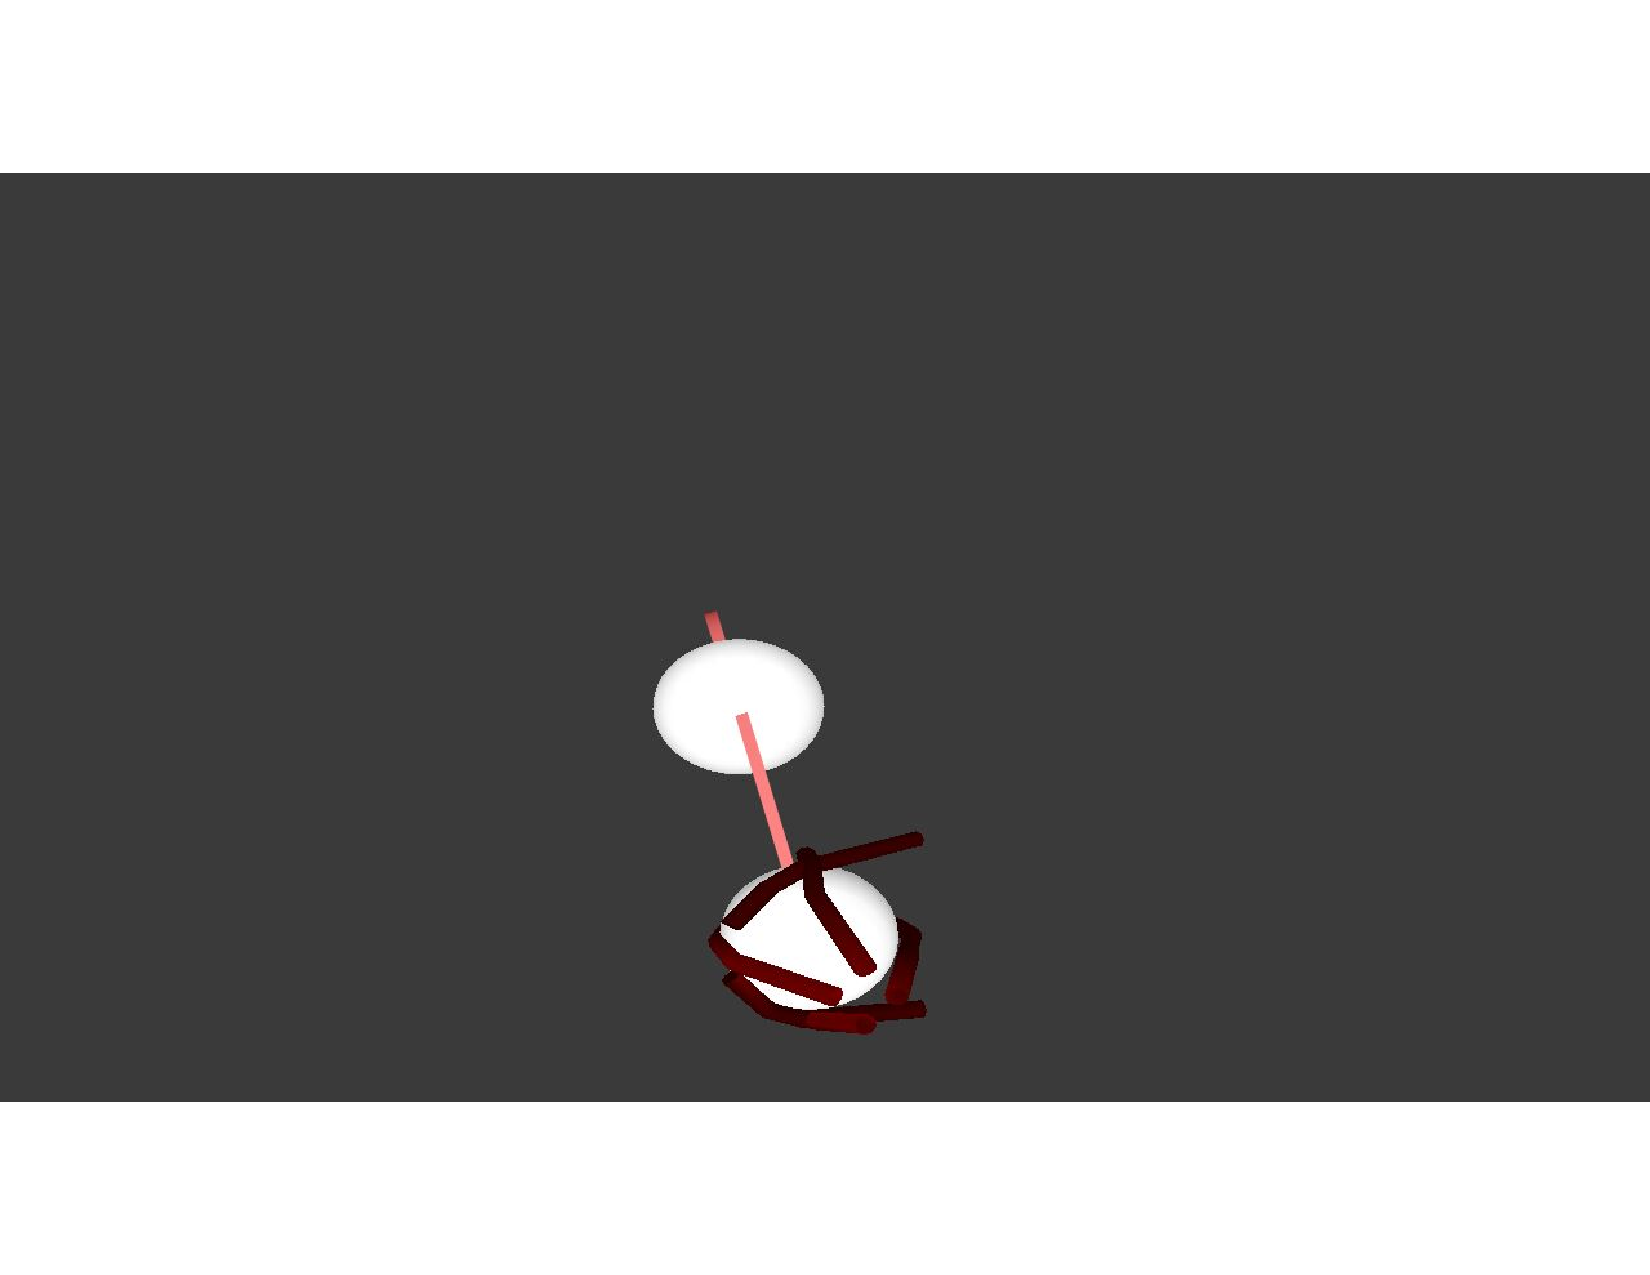
\includegraphics[width=\textwidth]{image000068}
         \caption{}
         \label{fig:ball_pos2}
     \end{subfigure}
    \caption[Target movement and corresponding gaze correction]{The ball moves from one point (a) to another (b). The red line reveals the current gaze direction, which shifts to the left and slightly downward between the two frames. This horizontal and vertical movement is encoded in the angles $\theta$ and $\phi$, respectively.}
    \label{fig:ball_movement}
\end{figure}

There are two viable methods for synthesizing eye movements---neuromuscular control as employed by \citet{Arjun} and inverse dynamic control. Because this thesis deals specifically with the foveation LiNet, we synthesize eye movements using inverse dynamics control. This starts with computing the angular position in which the eye needs to be in order to keep up with the moving visual target. Given the current angular position and desired angular position, we can compute the angular acceleration needed to complete the movement. From the angular acceleration we can compute the torque that the muscles need to produce and, finally, the muscle activations necessary to produce the desired torque. Although inverse dynamics control is less realistic than neuromuscular control, our goal is simply to prove that our SNN-based foveation network---dubbed the SLiNet---matches the performance of the existing LiNet foveation network.

To this end, we will test our SLiNet in accordance with the experimental regimen of \citet{Arjun}. This involves moving a visual target in three different ways and noting if the eye can successfully track it. The eye movements are defined as follows:
\begin{enumerate}
    \item \textit{Fixation}: The eye foveates the target while it remains fixed in space. The eye appears still and stable but may make small oscillatory movements. We test that these small oscillations exist as they enhance the biological plausibility of the model. 
    \item \textit{Saccade}: A quick eye movement that brings the visual target from peripheral vision to the central, foveal region of the retina. We test the extent to which our trained foveation SLiNet yields angular displacement, velocity, and acceleration similar to the previous LiNet model.
    \item \textit{Smooth pursuit}: Once the visual target is fixated upon, the eye can pursue the target as it moves freely in space, including approaching or receding from the eye. The trajectory of the eye movement should include realistic oscillations. We track the orientation of the eye through time to make sure that it successfully follows the target. Good performance here is an indication that the eye can track the target through many different trajectories.
    % \item \textit{Projectile Motion}: This is similar to smooth pursuit except that the target now changes size as it moves away from the eye. 

% We also quantitatively evaluate how well our SNN performs compared to the LiNet.

\end{enumerate}

%%%%%%%%%%%%%%%%%%%%%%%%%%%%%%%%%%%%%%%%%%%%%%%%%%%%%%%%%%%%%%%%%%%%%%

\chapter{Spiking Neurons}

% Image of ANN neuron
\begin{figure}
    \centering
    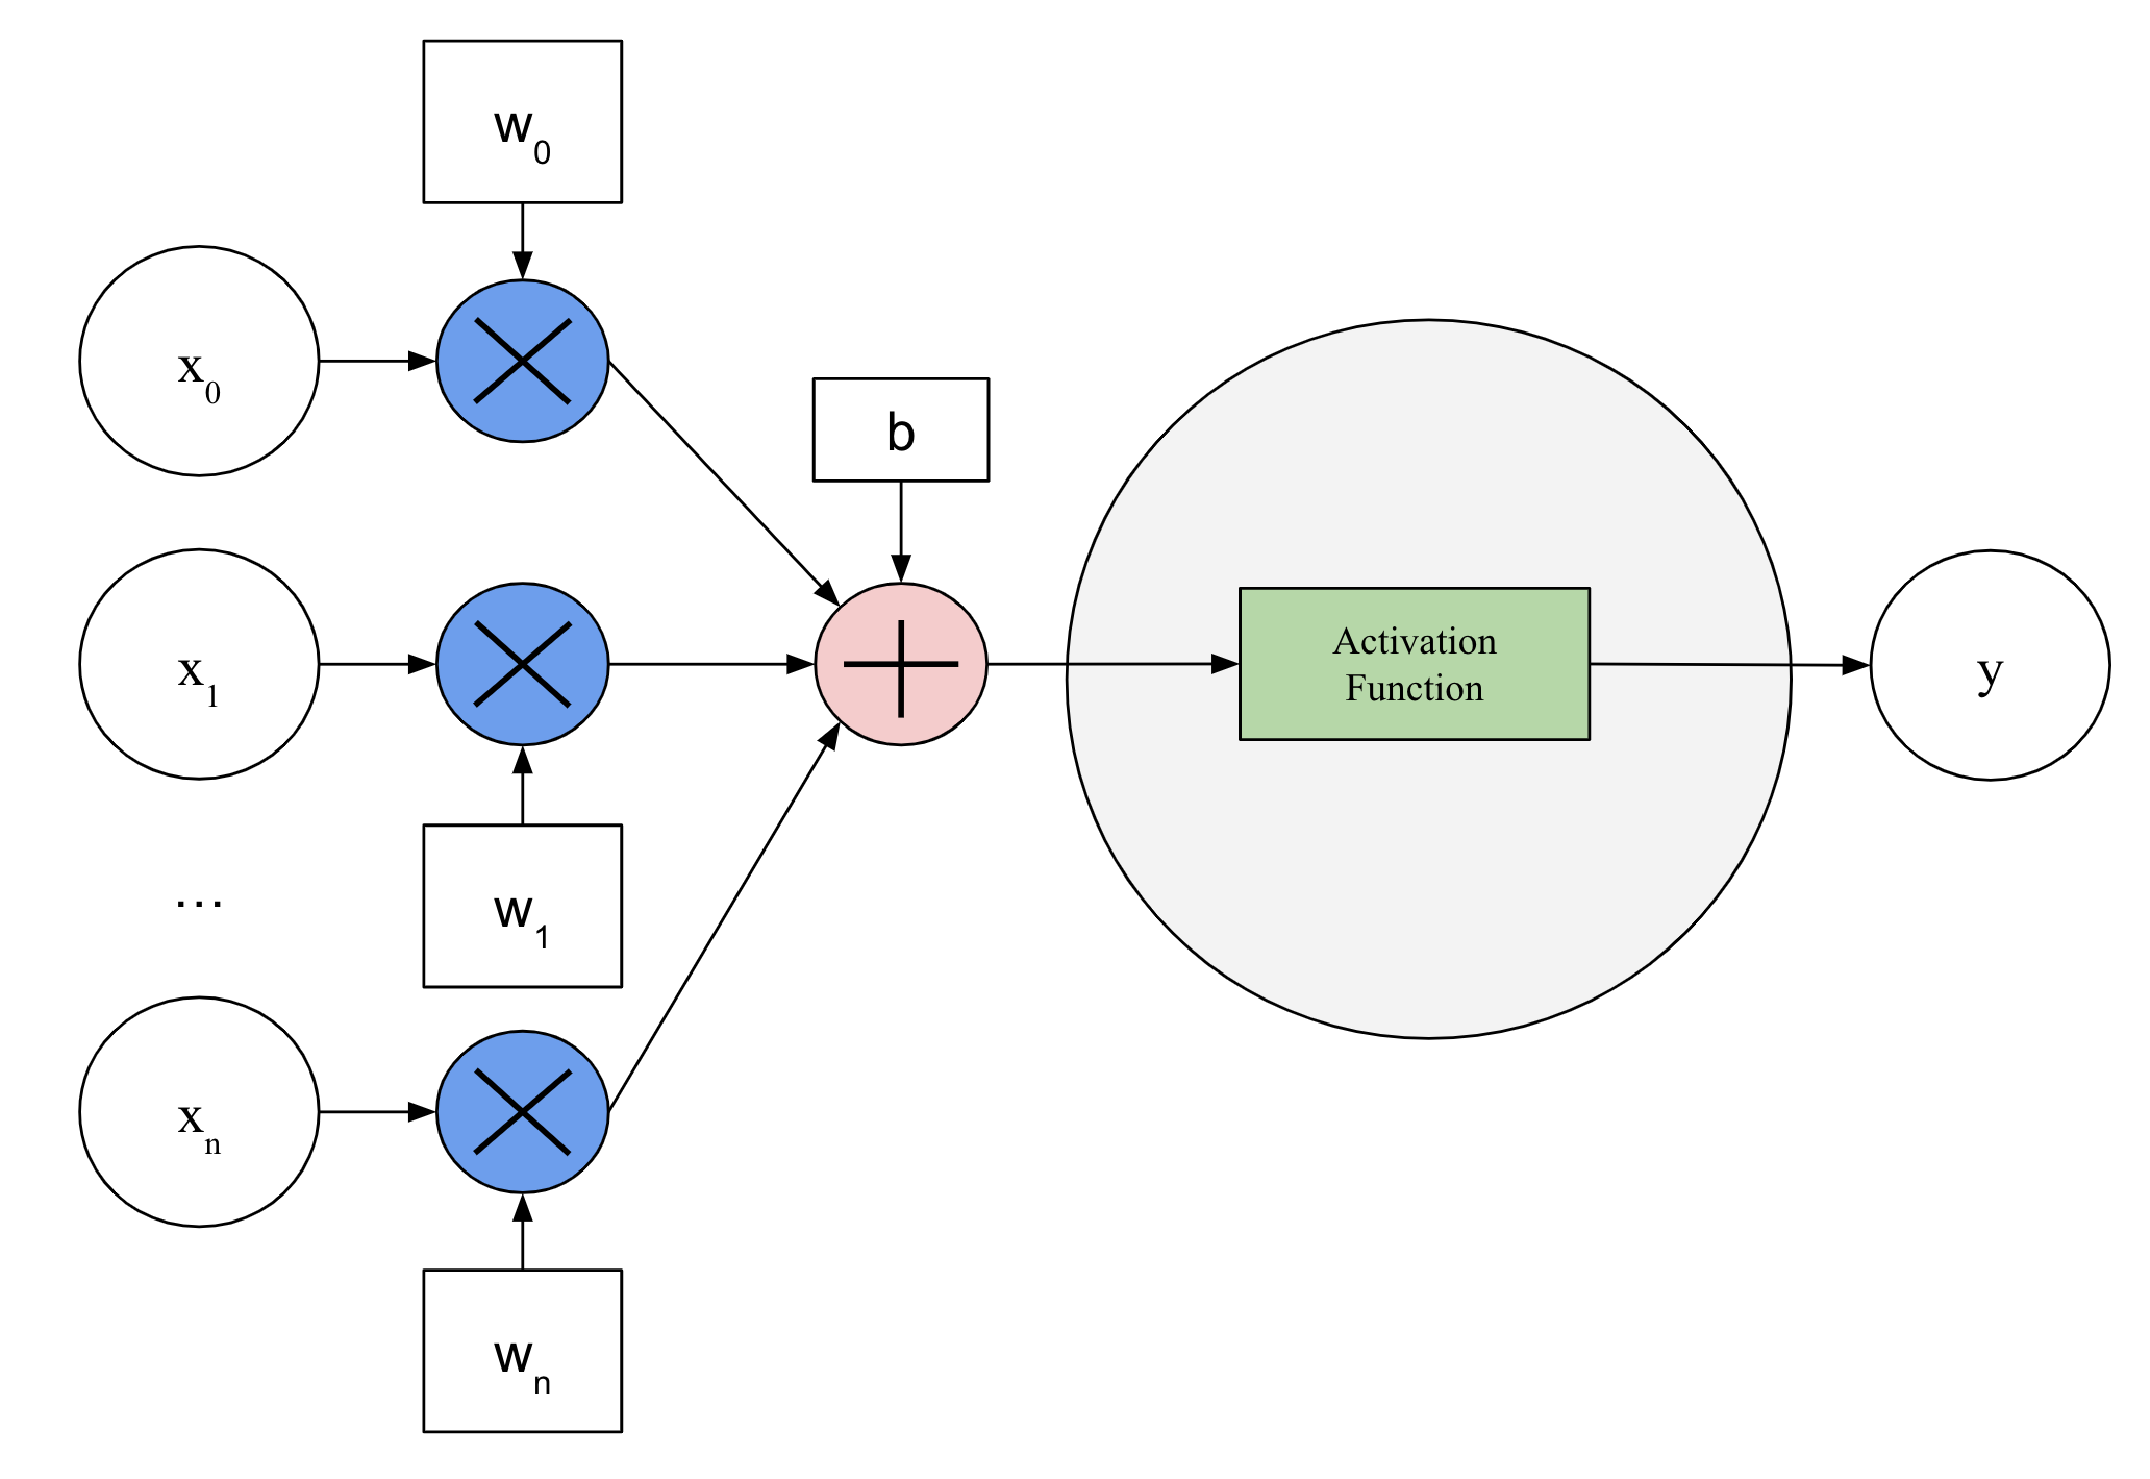
\includegraphics[width=0.7\textwidth]{neuron_ann}
    \caption[Artificial neuron model]{Internals of a conventional artificial neuron. The inputs, weights, and output are usually floating point numbers, whose multiplication requires multiply and accumulate (MAC) instructions, which typically consume considerable power.}
    \label{fig:neuron_ann}
\end{figure}

% Image of SNN neuron
\begin{figure}
    \centering
    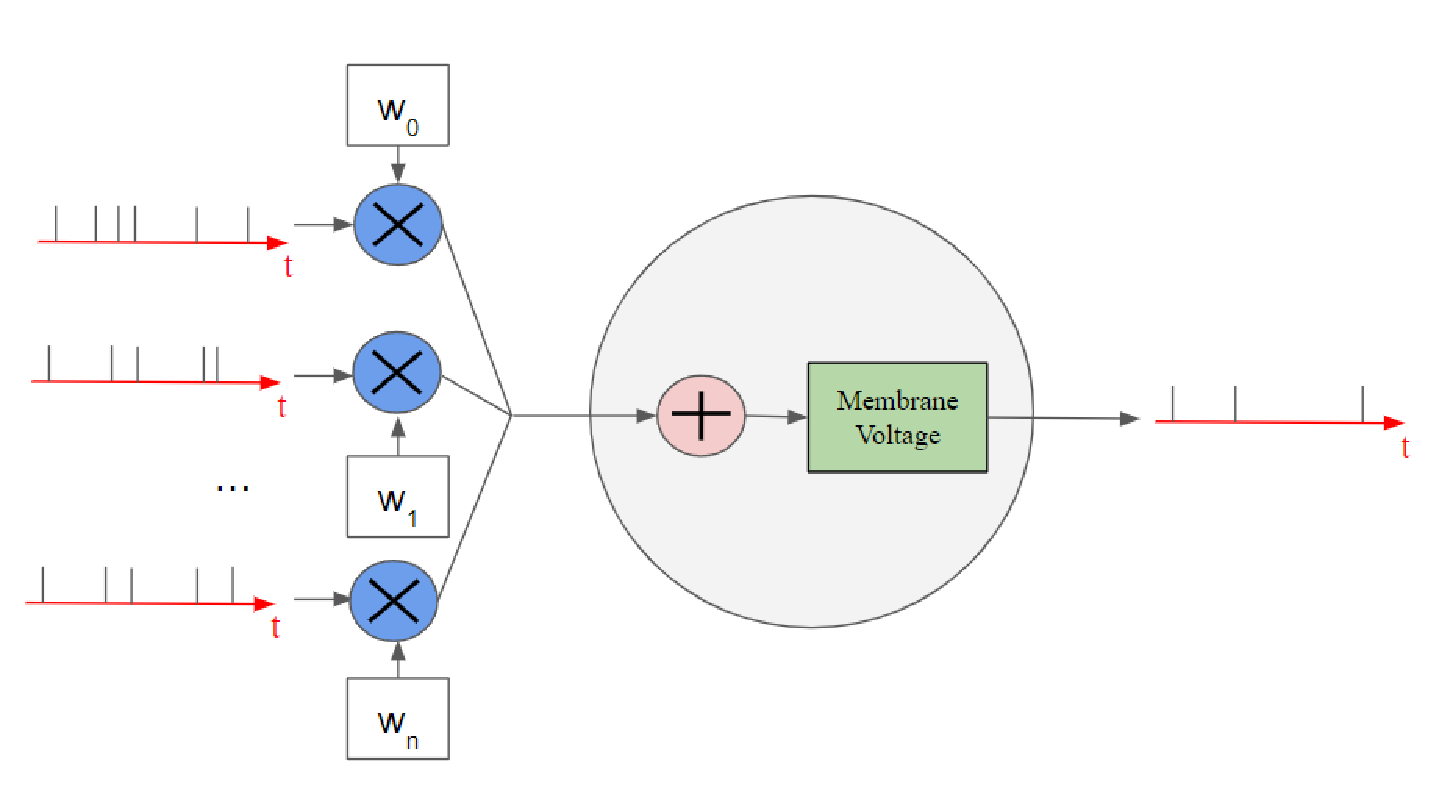
\includegraphics[width=0.8\textwidth]{neuron_snn}
    \caption[Spiking neuron model]{Internals of a spiking neuron. Each weight can only be multiplied by a 1 or a 0, eliminating the need for expensive MAC instructions.}
    \label{fig:neuron_snn}
\end{figure}

In this chapter, we introduce the basics of spiking neural networks. Additionally, we detail how to encode inputs to spiking neurons and interpret their outputs to perform a regression.

We first define the popular ANN currently in use. The corresponding neuron model is summarized in Figure~\ref{fig:neuron_ann}. In an ANN with $L$ layers, $W^l$, for $l \in 2,\dots, L$, is the weight matrix connecting layer $l-1$ to layer $l$. We multiply the output of the previous layer, $x^{l-1}$, with $W^l$, add biases $b^l$:
\begin{equation}
    a^l =  W^l x^{l-1} + b^l,
\end{equation}
and finally apply a rectified linear unit (ReLU) activation function:
\begin{equation}
    x^l = \max(0, a^l).
\end{equation}

Before moving on to a spiking neuron, which is illustrated in Figure~\ref{fig:neuron_snn}, we define some terms. A synapse refers to the connection between two neurons which has an associated weight $w$ that is tuned during training. Looking at a specific neuron, all neurons in the previous layer that are connected to it are referred to as presynaptic neurons and all neurons connected to it in the next layer are postsynaptic neurons. The inputs are time varying and in the form of spike trains, which are sequences of 1's and 0's. All spike trains in the network are the same length, which is treated as a hyperparameter.

% Image of input spikes, corresponding voltage increasing and decaying, and output spikes
\begin{figure}
    \centering
    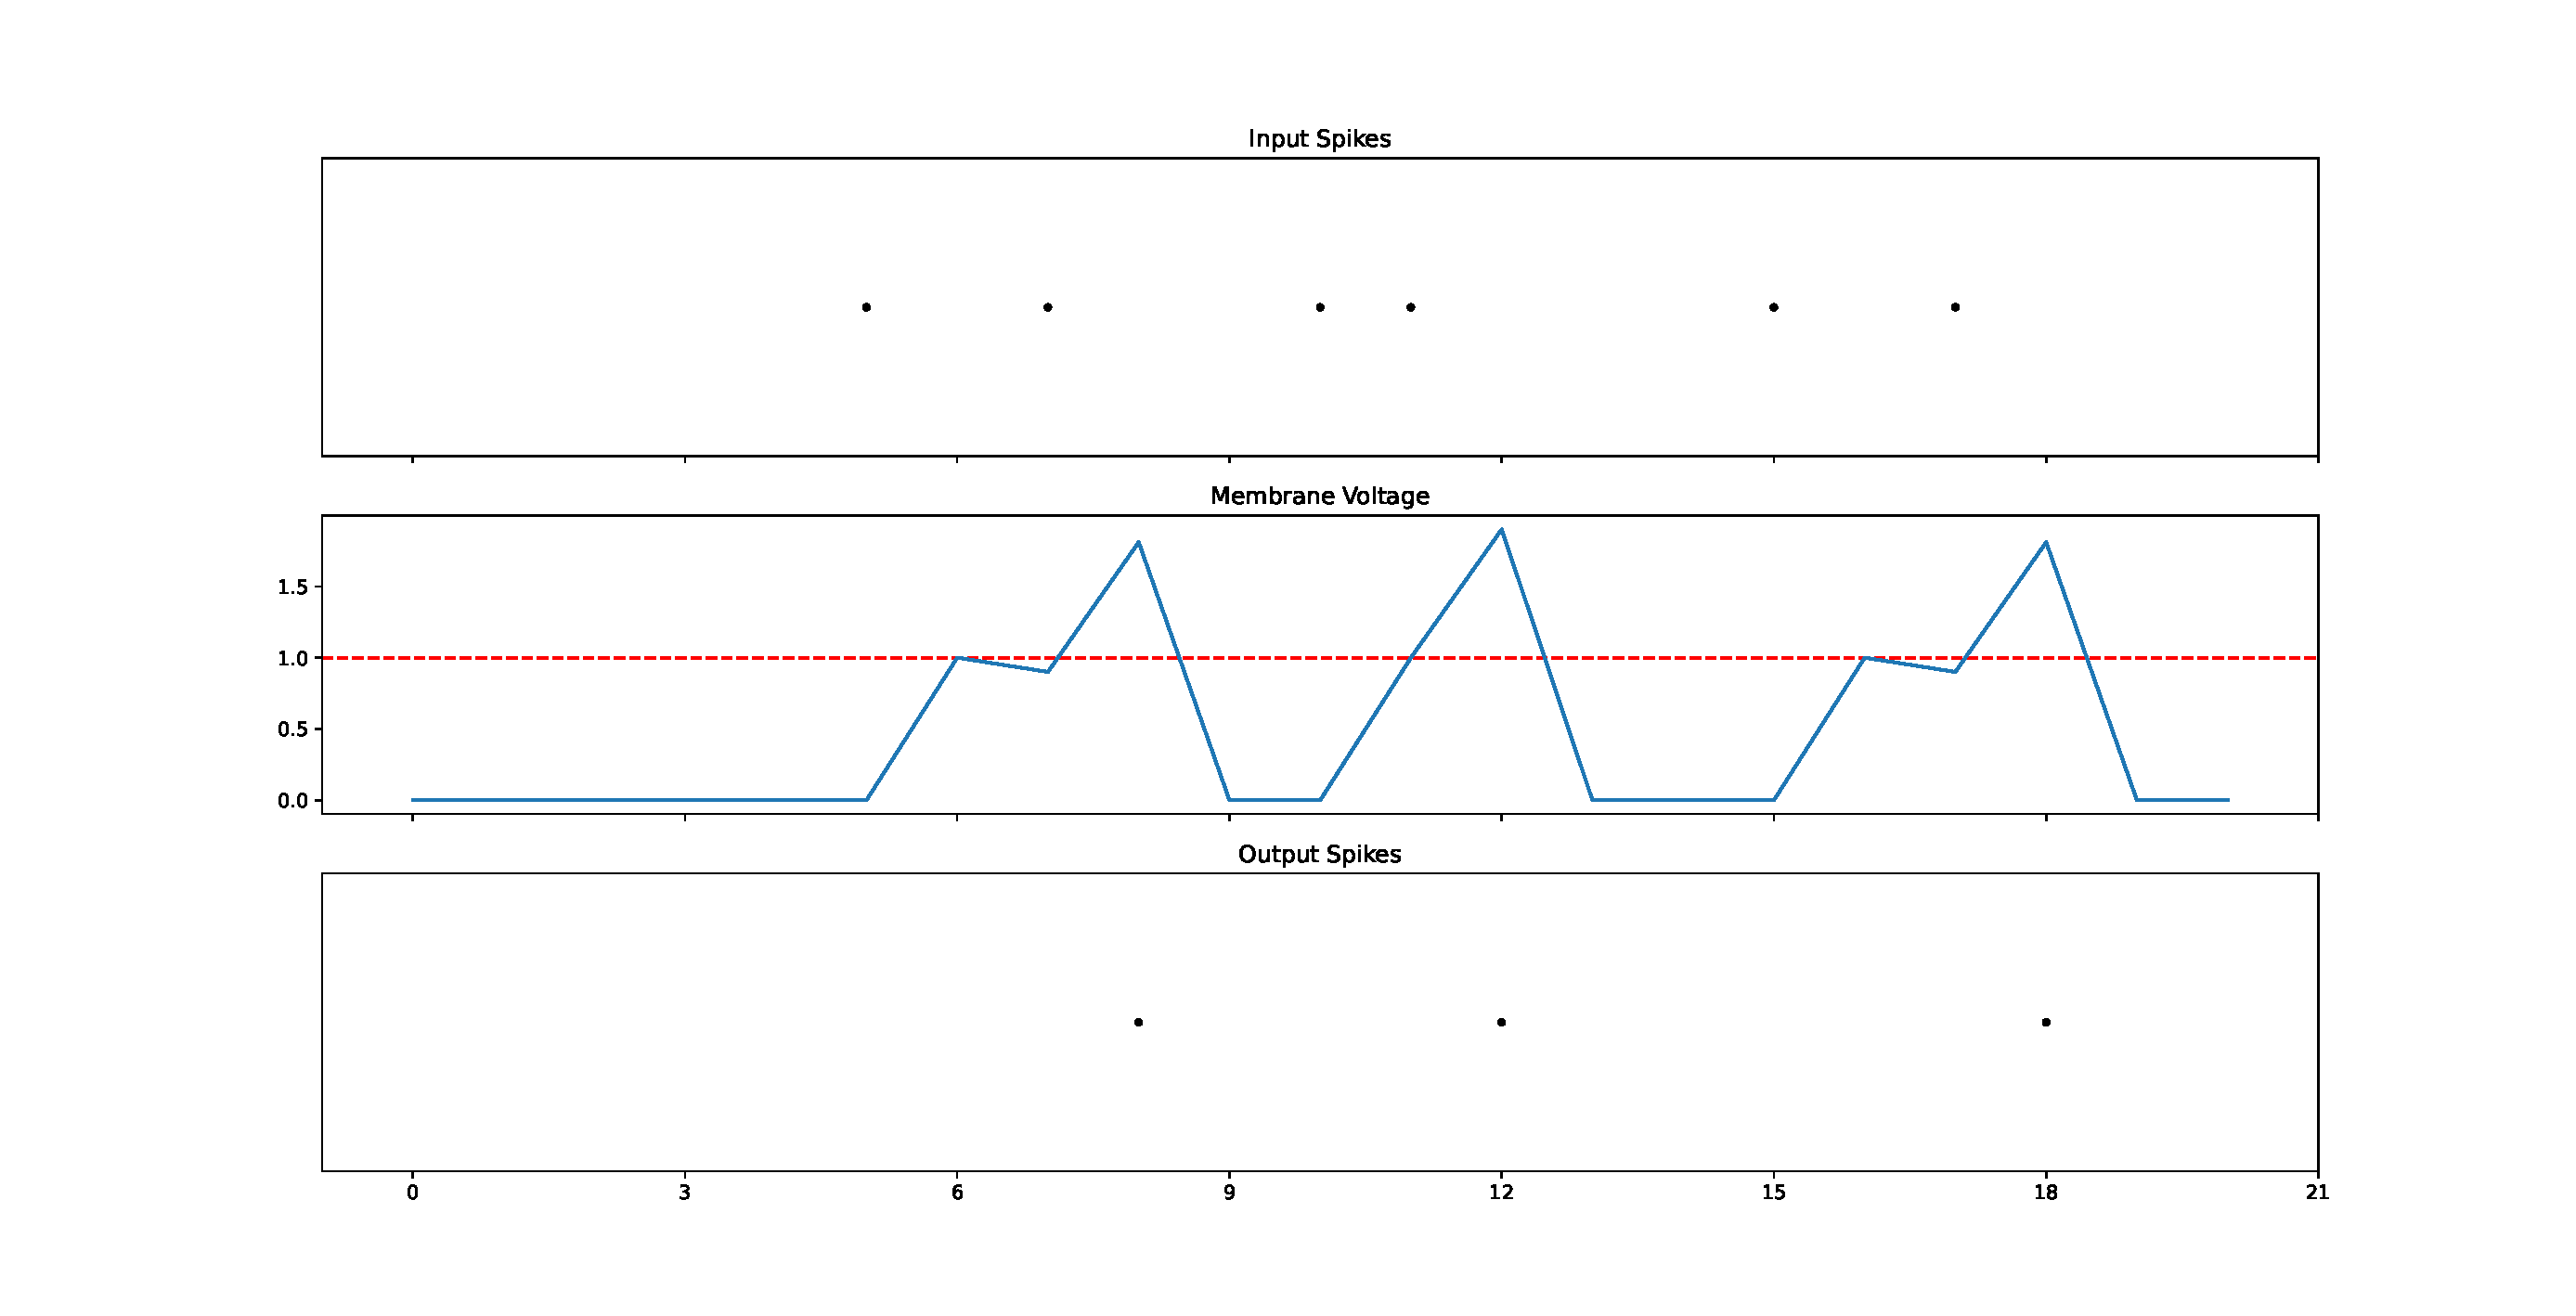
\includegraphics[width=\textwidth]{snn_spike_example}
    \caption[Demonstration of a Leaky Integrate-and-Fire (LIF) neuron]{Demonstration of a LIF neuron. Input spikes to the neuron are at the top, the neuron's membrane voltage is in the middle, and output spikes are at the bottom. The threshold voltage is denoted by the dashed red line. We verify that the membrane voltage increases when there is an input spike and that there is an output spike when the membrane voltage crosses the threshold. A reset occurs after each output spike, represented by the steep decrease in the membrane voltage. There is also a slight leak of membrane voltage in the absence of any input spikes (such as around timestep 6).}
    \label{fig:lif_spike_example}
\end{figure}

Each spiking neuron maintains a state variable known as the membrane voltage
\begin{equation}
U(t) = \underbrace{\beta U(t-1)}_{\text{decay}}
+ \underbrace{W X(t)}_{\text{input}}
- \underbrace{S(t-1)U_T}_{\text{reset}},
\end{equation}
where matrix $W$ stores the weights and tensor $X$ stores the presynaptic inputs, and where the spiking activation function is $S(t)$.
\begin{equation}
S(t) = \begin{cases} 
      1 & \text{if } U(t) > U_T \\
      0 & \text{otherwise }
      \end{cases}
      = \mathcal{H} (U(t) - U_T)
\end{equation}
$U(t)$ used to calculate the membrane voltage of a neuron at timestep $t+1$. If a presynaptic neuron spikes, we add the corresponding synapse weight to this membrane voltage. If no spikes are input to the neuron, the membrane voltage decays exponentially. This decay is controlled with the hyperparameter $\beta$. If $U$ exceeds a certain threshold $U_T$, then the neuron outputs a spike and resets $U$ to zero. This spiking behavior is captured by the Heaviside step function, represented by $\mathcal{H}$. 

The membrane voltage equation is used by snnTorch \citep{snnTorch}, a Python package built on top of PyTorch, which we employ in our work. This neuron model is known as the leaky integrate-and-fire (LIF) neuron, so named because it ``leaks'' voltage in the absence of an input. Figure~\ref{fig:lif_spike_example} demonstrates how membrane voltage is calculated with an example LIF neuron. 

To summarize, an SNN differs from the conventional ANN in two fundamental ways. First, we replace the activation function with one that only outputs 1's and 0's. Second, we have inputs that vary over time. More detailed derivations of SNN theory can be found in Appendix \ref{appendix:snn}.

%********************************************************************%

\section{Encoding Input Signals}

As stated previously, our ONV is a vector of dimension 43,200. SNNs, however, expect inputs that vary over time. In addition, the floating point numbers that represent the RGB light intensity at any retinal photoreceptor need to be meaningfully converted into ``spikes;'' i.e., a series of 1's and 0's. This is known as converting data from the ``frame'' domain to the ``spiking'' domain, and we explore two main conversion schemes.

\begin{figure}
    \centering
    \begin{subfigure}{0.49\textwidth}
        \centering
        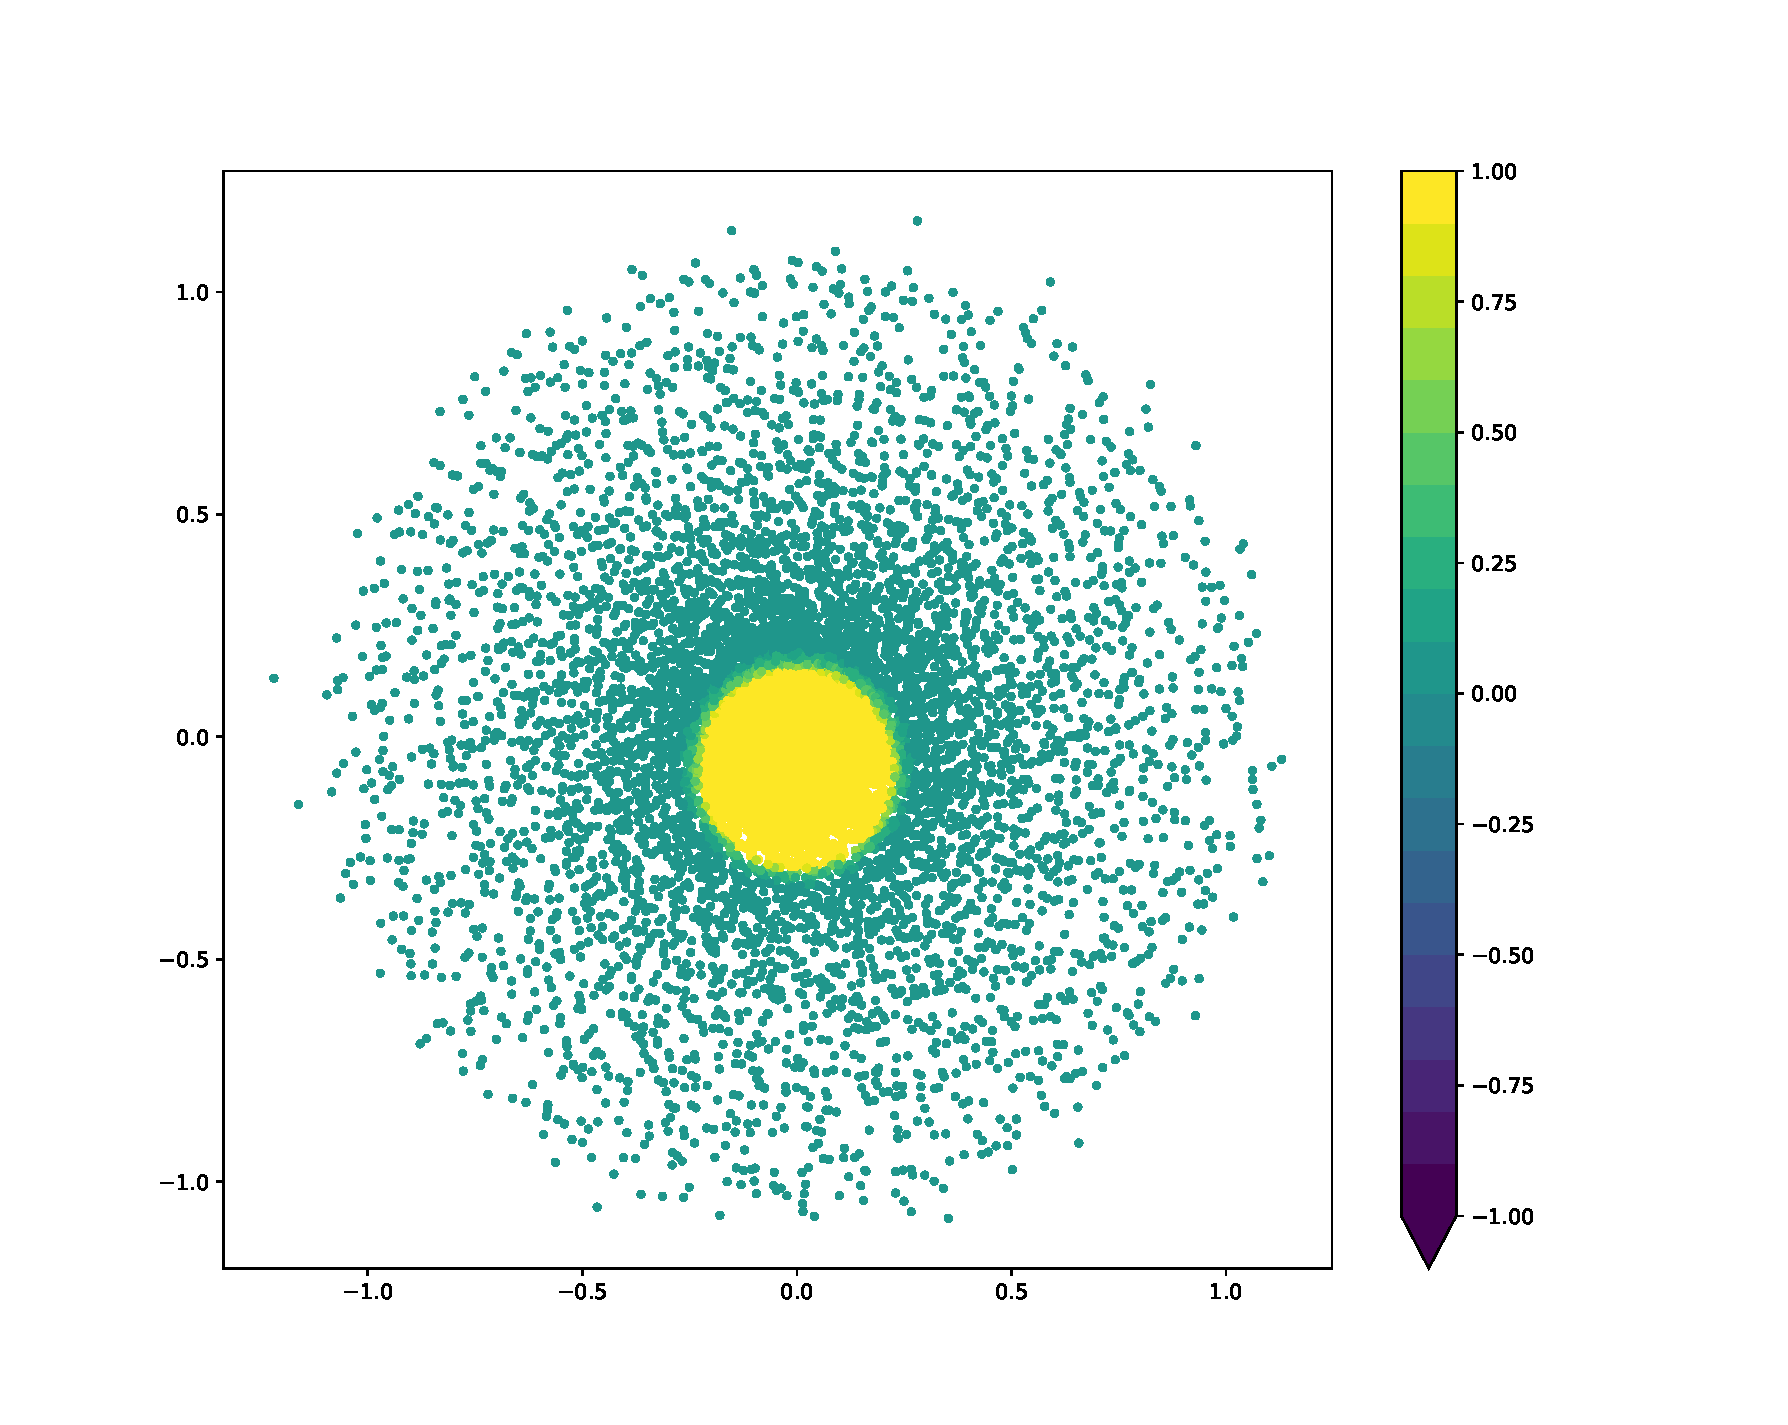
\includegraphics[width=\textwidth]{onv_normal_prev}
        \caption{Previous ONV}
        \label{fig:onv_prev}
    \end{subfigure}
    \hfill
    \begin{subfigure}{0.49\textwidth}
        \centering
        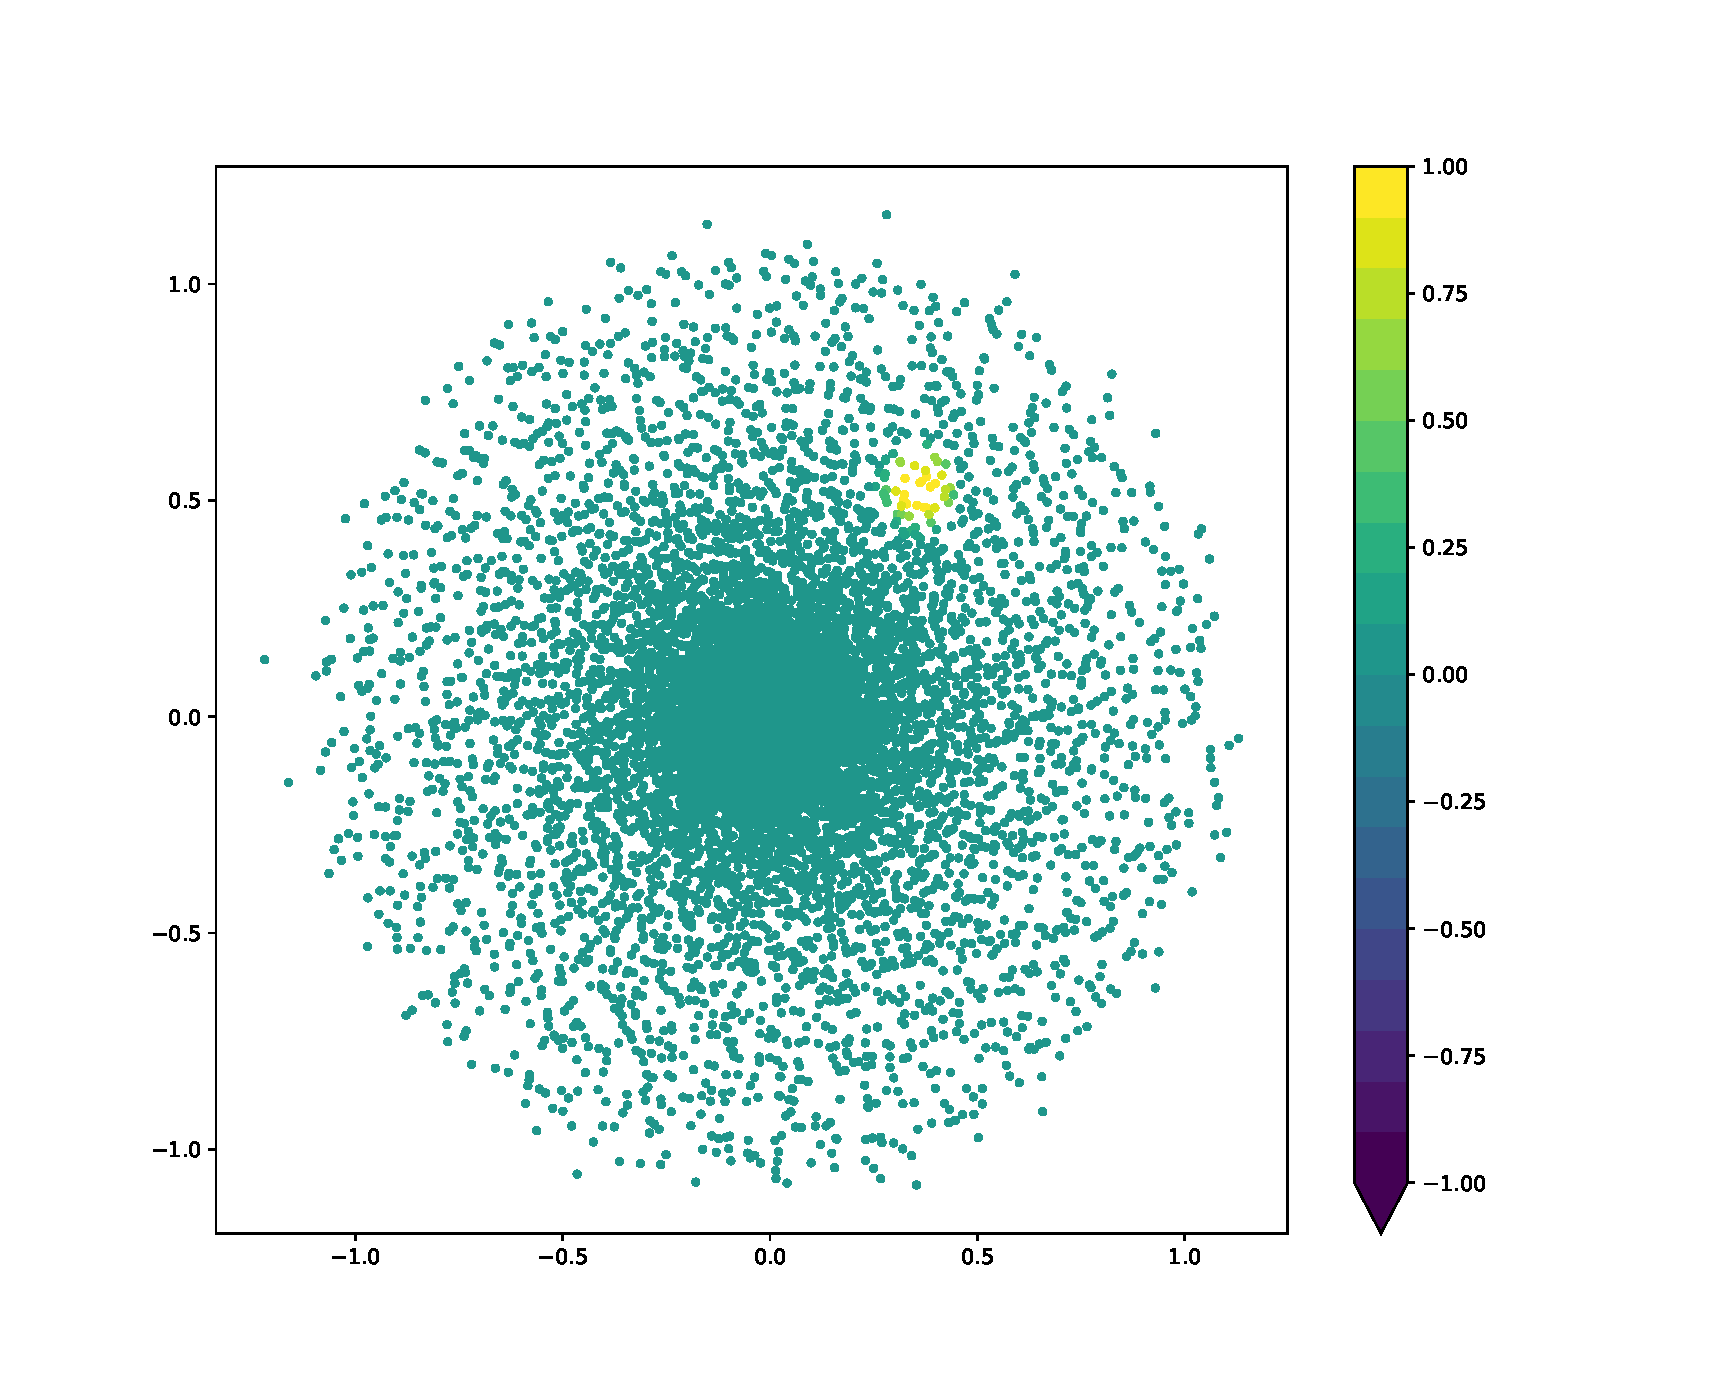
\includegraphics[width=\textwidth]{onv_normal_cur}
        \caption{Current ONV}
        \label{fig:onv_cur}
    \end{subfigure}
    \hfill
    \begin{subfigure}{0.49\textwidth}
        \centering
        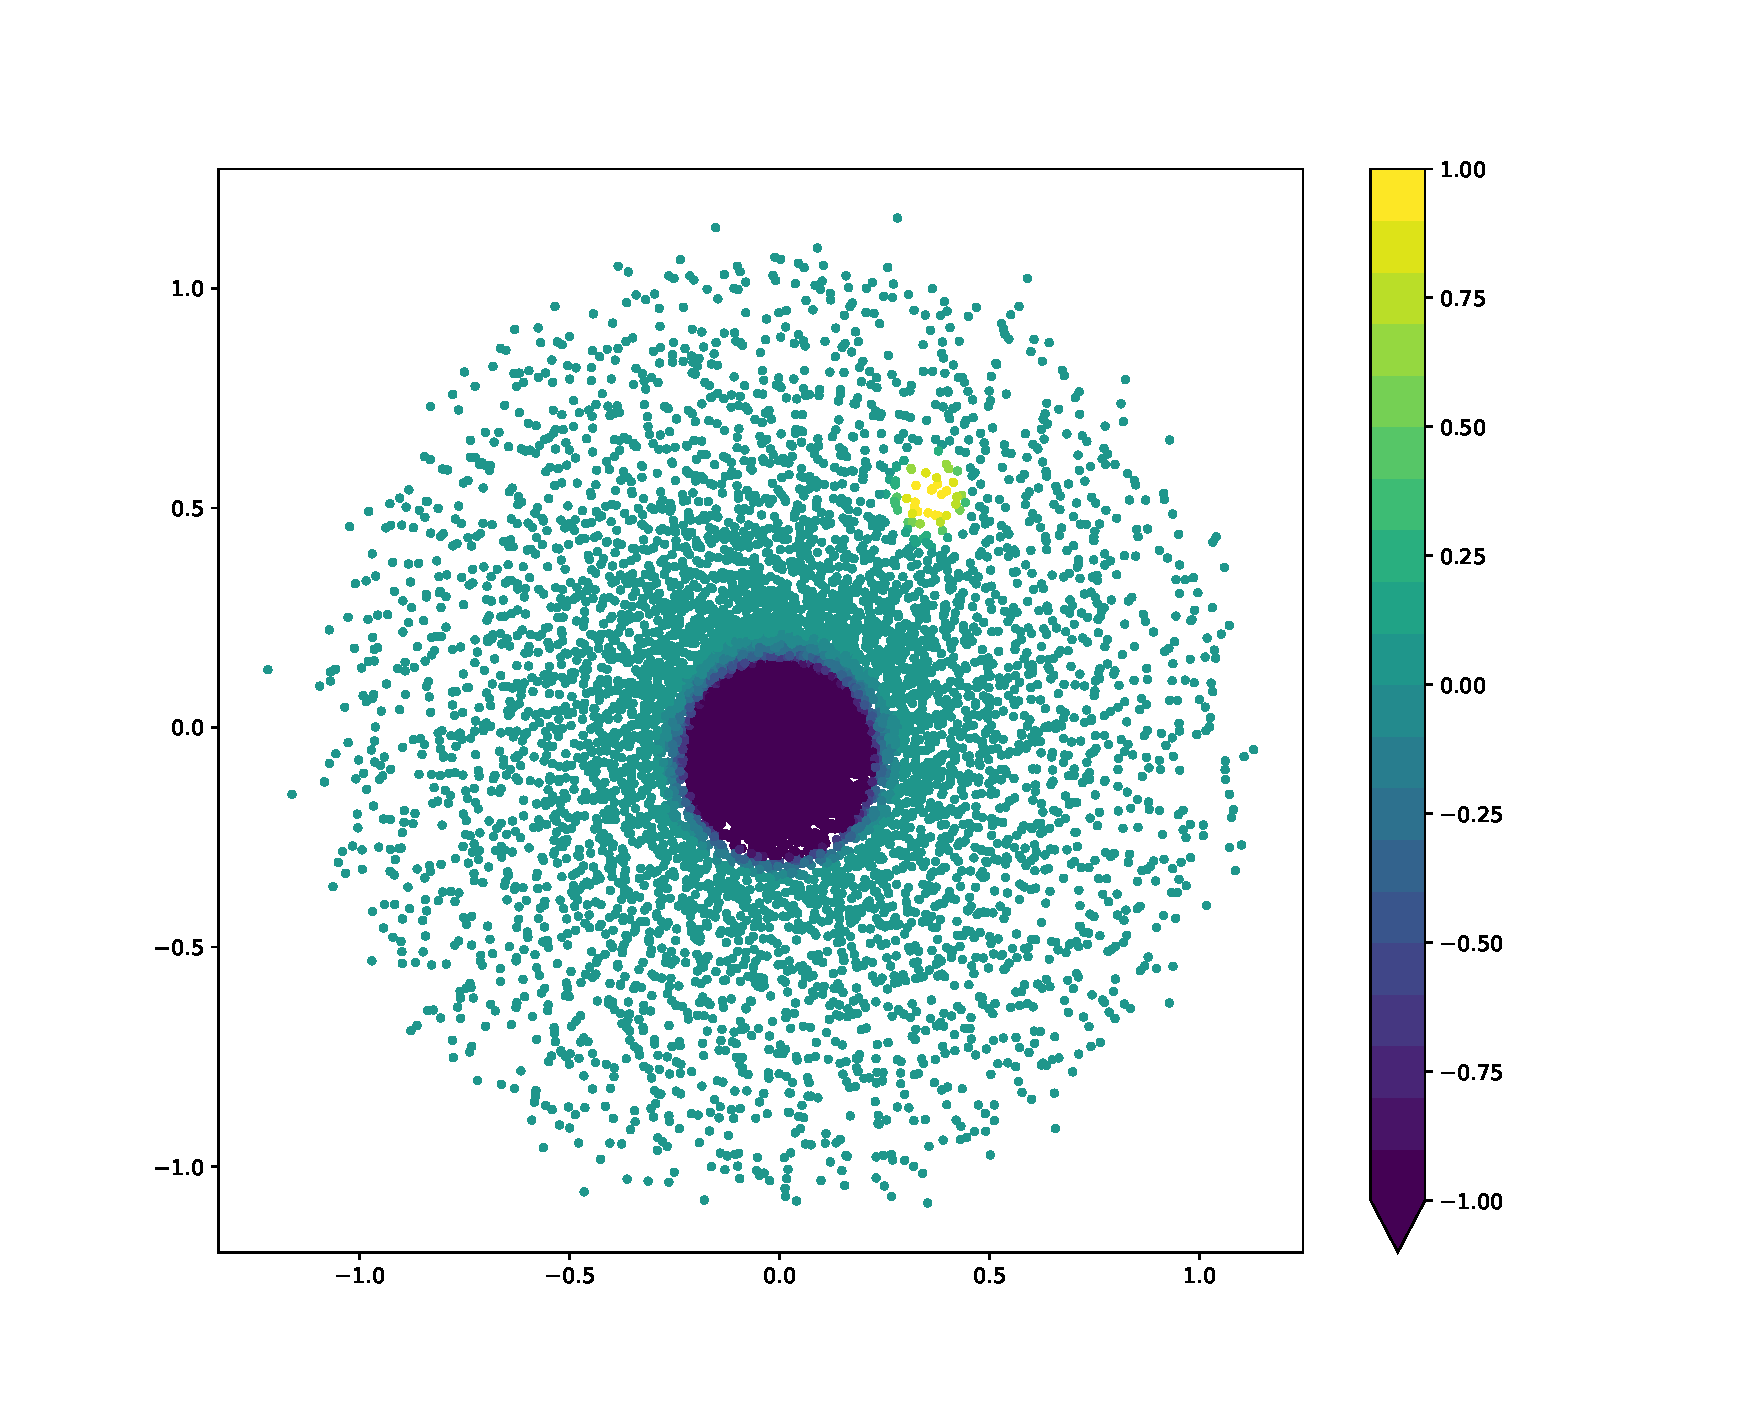
\includegraphics[width=\textwidth]{onv_delta}
        \caption{D-ONV}
        \label{fig:onv_delta}
    \end{subfigure}
    \caption[ONV and D-ONV for a moving target]{We map ONV values collected from a scene by the photoreceptor distribution. Note that ONV values are in the range $[0,1]$ while D-ONV values are in the range $[-1,1]$. The target has moved from one position in (a) to another in (b). (c) shows the corresponding D-ONV. The values darken where the target was in (a) and get brighter at the target's location in (b). }
    \label{fig:three ONVs}
\end{figure}

\begin{figure}
    \centering
    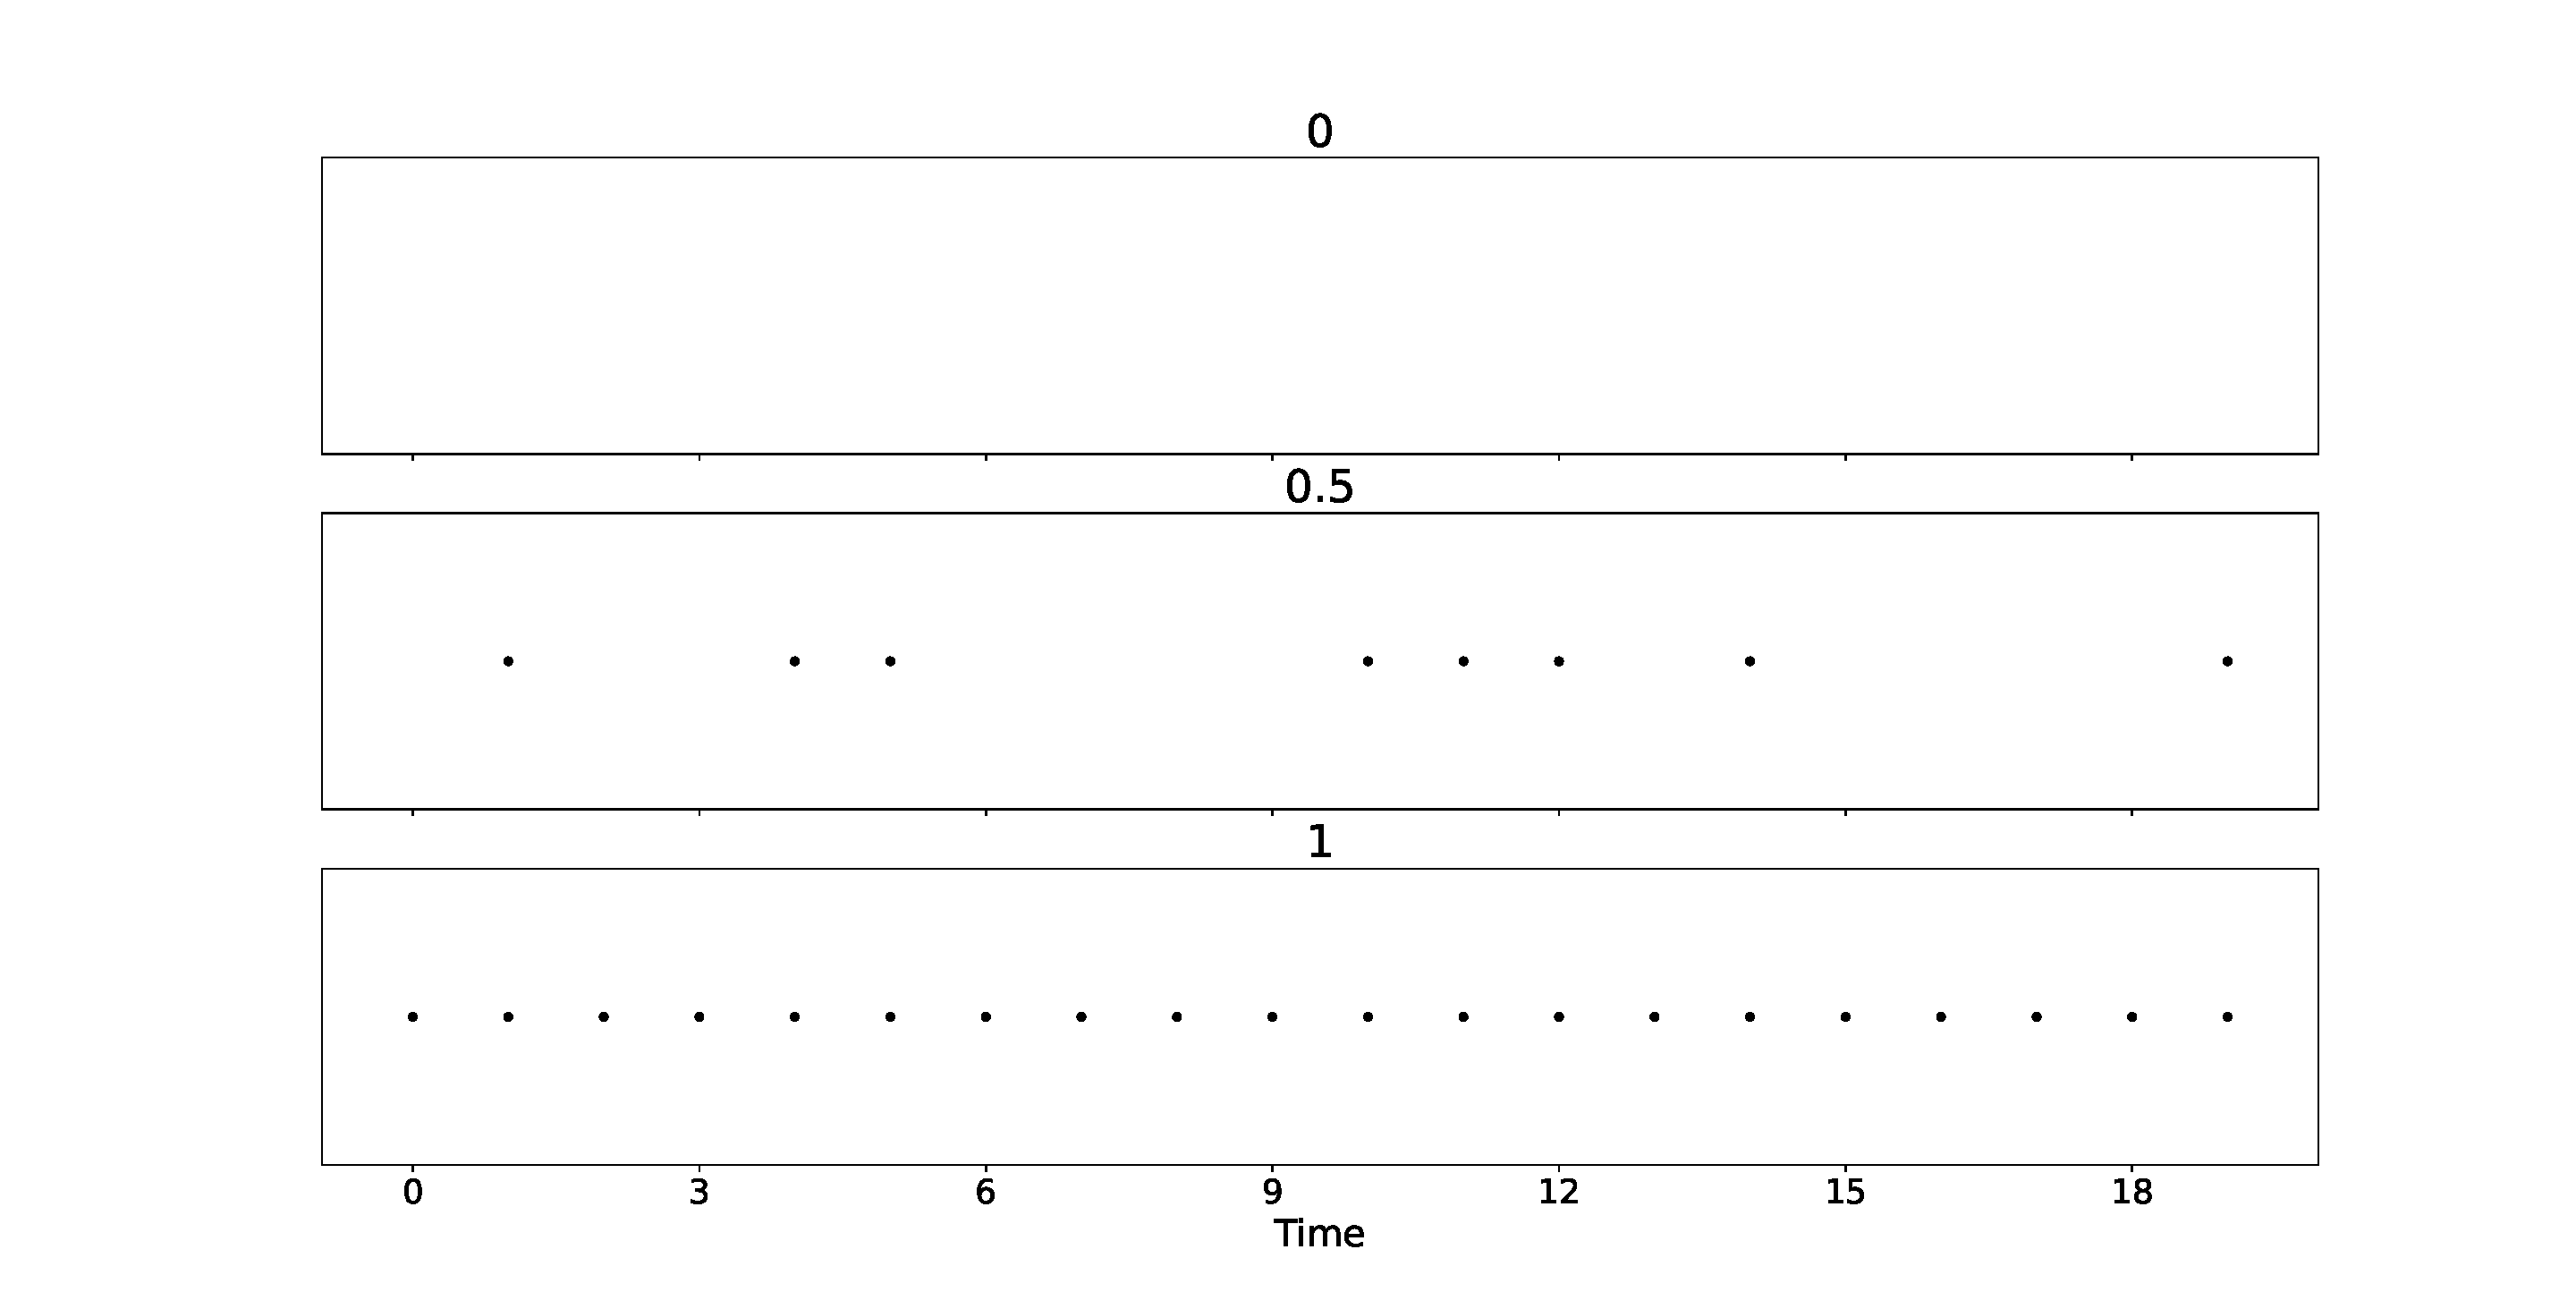
\includegraphics[width=1.0\textwidth]{neuron_3_rate}
    \caption[Rate encoding with Bernoulli trials]{Demonstration of rate encoding with Bernoulli trials. From top are encoded data values of 0.0, 0.5, and 1.0.}
    \label{fig:rate_encode_3plots}
\end{figure}

In addition to generating spiking inputs, we also introduce what we refer to as the Delta-ONV, or D-ONV for short; instead of having the eye see light intensities at the current timestep, it sees the \emph{difference} between the current and previous ONV values, as shown in Figure~\ref{fig:three ONVs}. In other words, the eye detects only the changes in the scene that manifest in intensity changes at the retinal photoreceptors. These changes are also referred to as ``event-based'' data. Note that the D-ONV exhibits positive values at photoreceptors that register brighter and negative values if they register darker. This results in sparse input data as the eye need not repeatedly re-process what it has already observed. The D-ONV is more biologically accurate, since ganglion cells in the retina emit spikes only when there is an intensity change in the field of view \citep{eventRetina}.

% do I need this higher level organization?

Next we review the two most popular encoding methods, rate and latency encoding. It is still unknown exactly how neurons encode various stimuli into spikes, but it is believed that each method is used in different parts of the brain, including in the visual cortex. \citet{spike_encoding_real_retina} find that retinal ganglion cells use different encoding methods for different tasks. We empirically found that rate encoding performed better than latency encoding on our object tracking task.

%********************************************************************%

\subsection{Rate Encoding}

Rate encoding attempts to encode a neuron's firing frequency. Each input value to the encoder lies in the range between 0 and 1, representing the probability that the neuron will spike at a given timestep. Then, at each timestep, we run a Bernoulli trial with the given probability to determine if the neuron will spike. For example, if our photoreceptor intensity value was 0, the neuron would never spike. On the other hand, a value of 1 would create spikes at each timestep. A value of 0.5 would result in approximately half of the timesteps containing a spike. We show these examples over 20 timesteps in Figure~\ref{fig:rate_encode_3plots}.

\begin{figure}
    \centering
    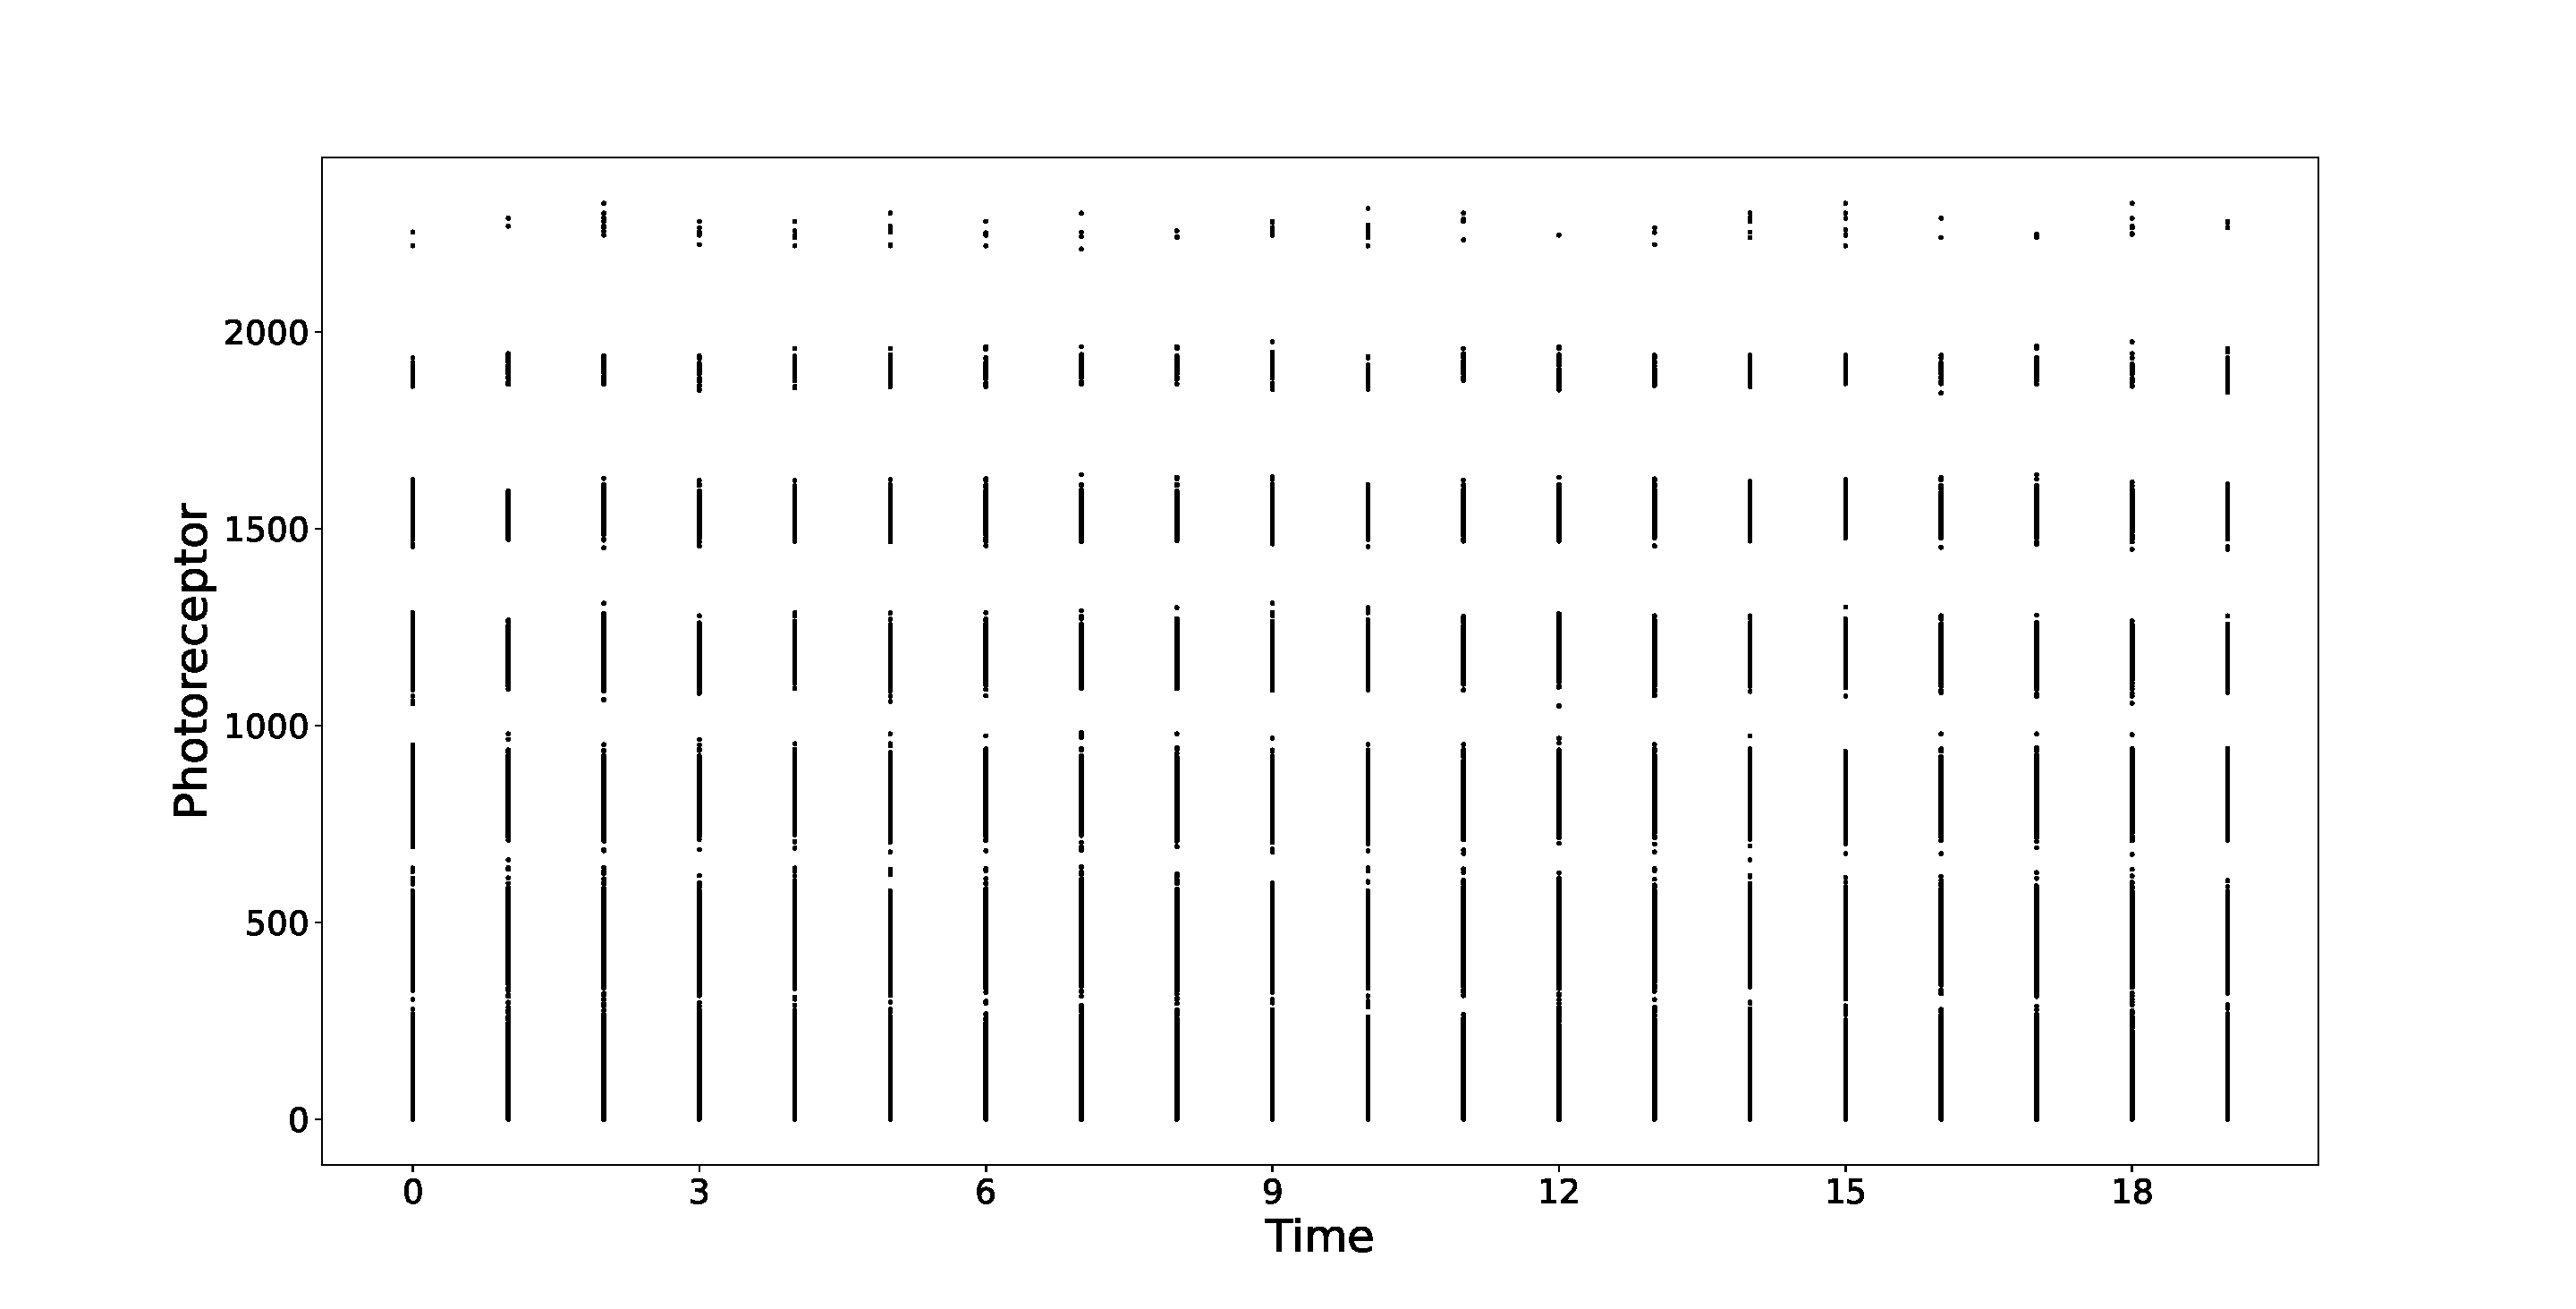
\includegraphics[width=1.0\textwidth]{onv_rate_prev}
    \caption[Rate encoded ONV]{Rate encoding of a subset of photoreceptors from the ONV in Figure~\ref{fig:onv_prev}. Each horizontal line represents the spiking behavior of one photoreceptor. Only the photoreceptors with nonzero inputs are spiking, and we can see different spike rates corresponding to different light intensities.}
    \label{fig:onv_encode_rate}
\end{figure}

Each of our RGB color channels are already in the range of 0 to 1, so they can directly be rate encoded. In Figure~\ref{fig:onv_encode_rate} we present a subset of the input spikes that result from rate encoding the ONV from Figure~\ref{fig:onv_prev}. We can see a few different firing rates in the figure, with excited neurons firing at every timestep and other neurons not firing at all.

With the D-ONV, however, we have values in the range of -1 to 1. This is a problem because we cannot have a negative probability assigned to whether or not an input neuron will spike. The solution is to take the absolute value of the probability, and if a spike is generated, it will carry a value of -1 instead of 1. This means that neurons in the next layer will decrease their internal voltages if they receive a spike with value -1. Figure~\ref{fig:negative_spike_example} shows what happens when a neuron receives negative spikes as input.

\begin{figure}
    \centering
    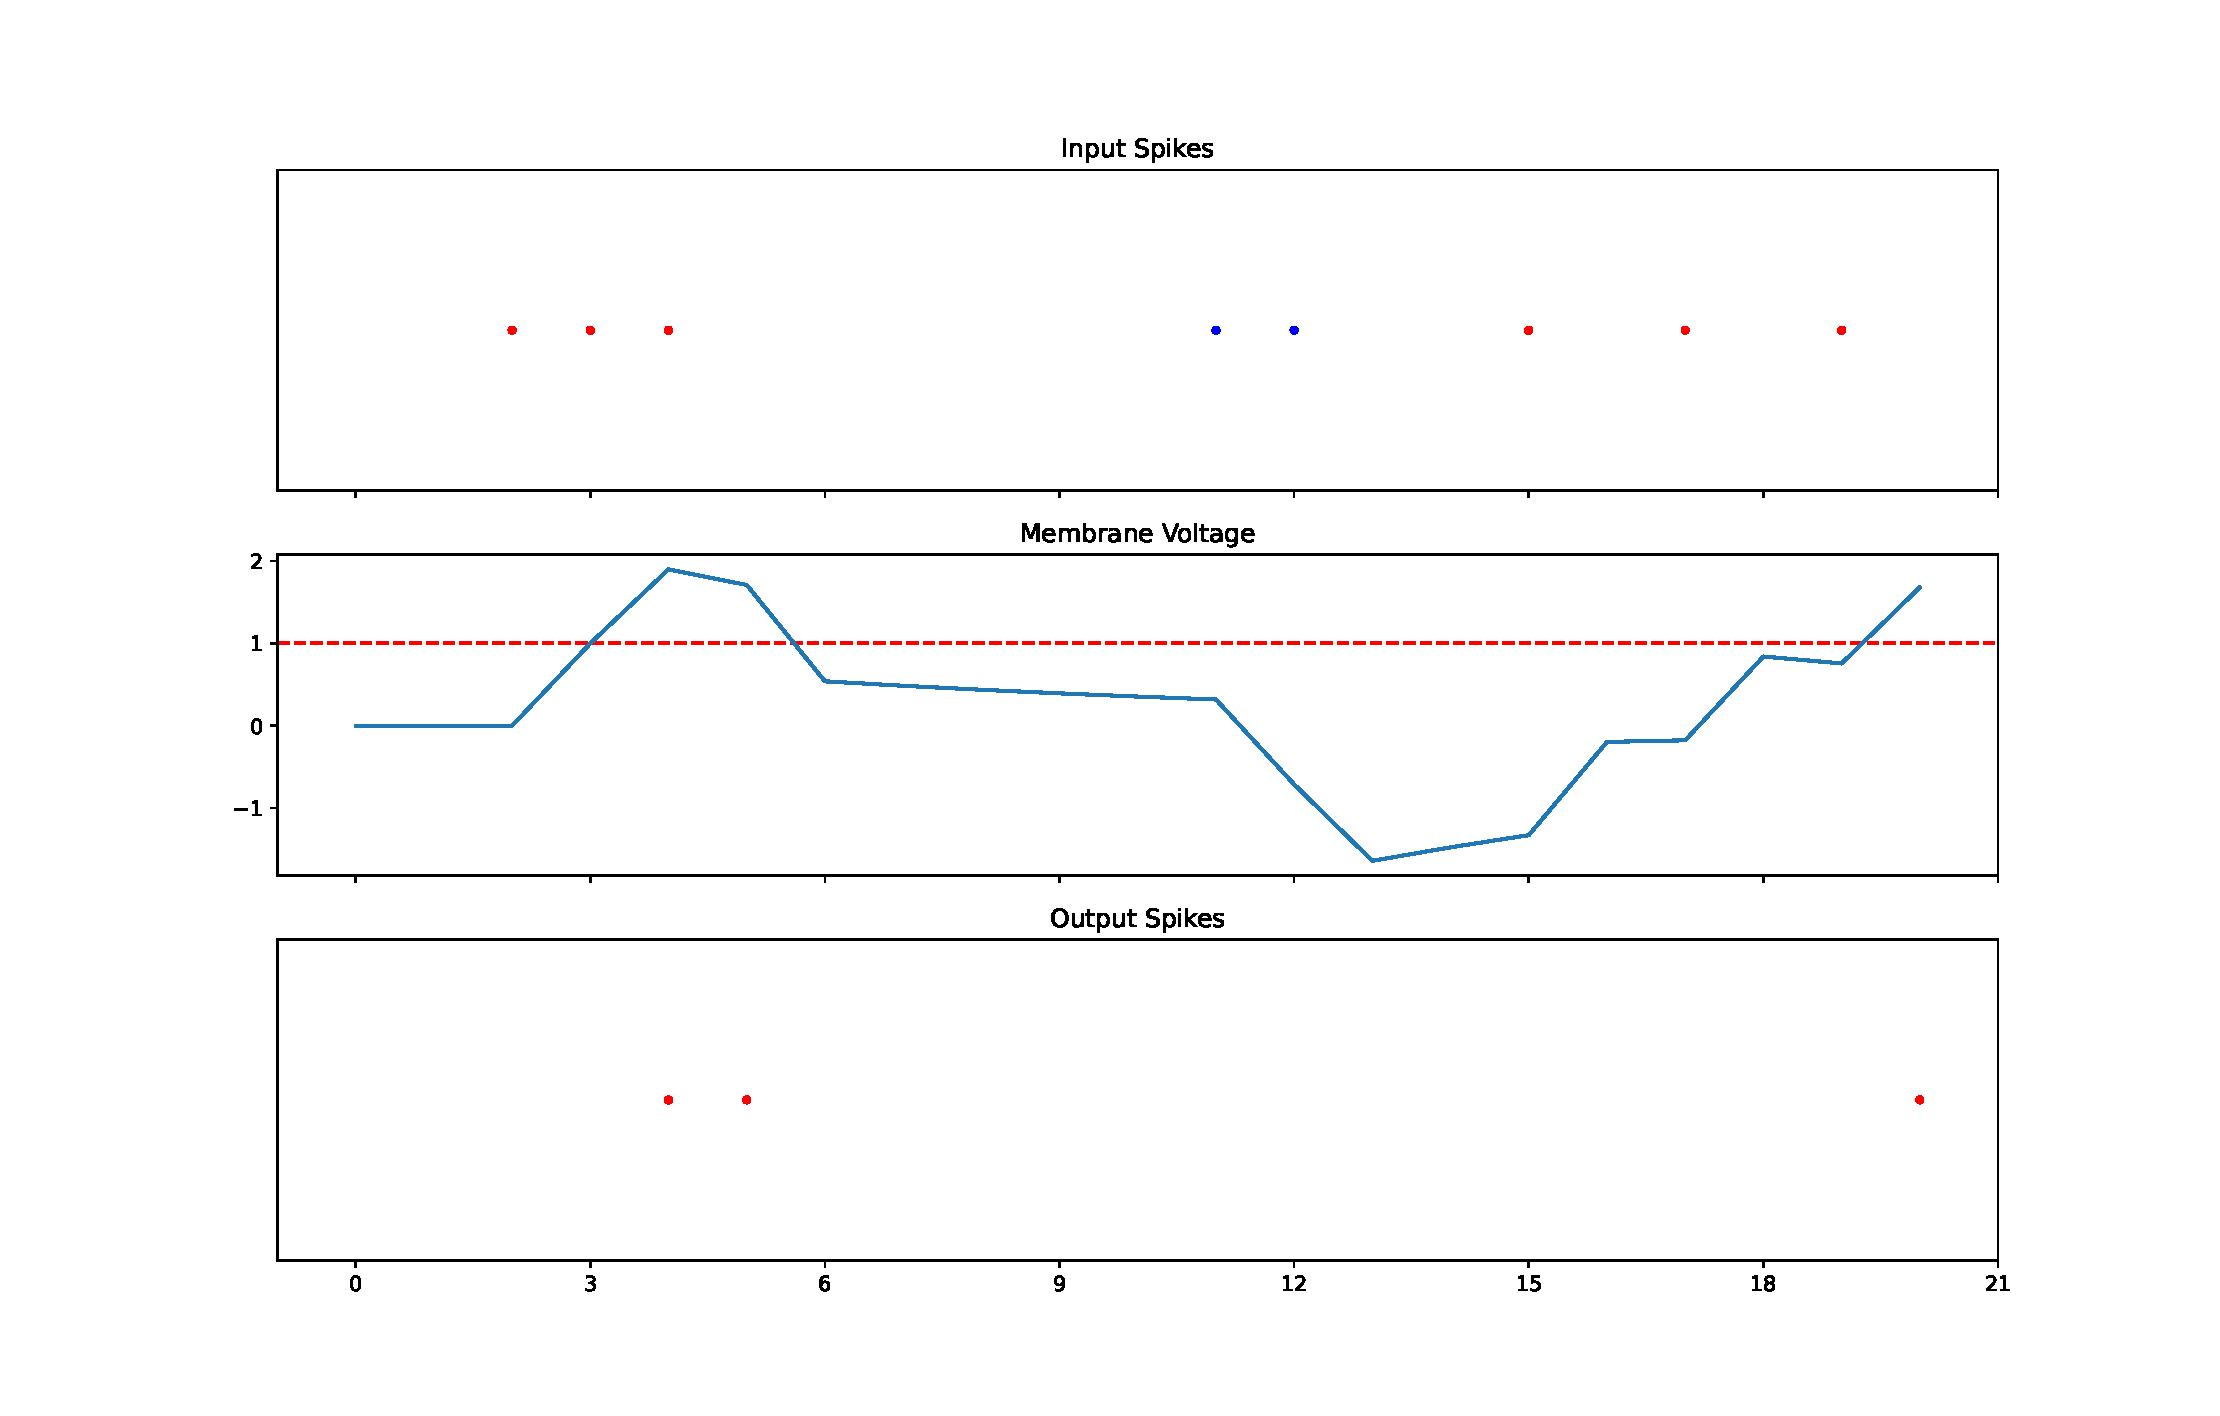
\includegraphics[width=\textwidth]{negative_spike_example}
    \caption[Negative spike inputs to a LIF neuron]{A LIF neuron that receives both positive (red) and negative (blue) spikes as input. The membrane voltage increases with positive input spikes and crosses the threshold voltage to output spikes. Around timestep 5 the neuron resets, but there is also another input spike. This spike adds to the membrane voltage, causing it to stay above the threshold after the reset. When the negative spikes arrive as input, the membrane voltage decreases.}
    \label{fig:negative_spike_example}
\end{figure}

The inputs to the rate encoder can also be scaled up before being turned into spikes. This is referred to as the gain, which we treat as a hyperparameter. For example, given gain $g$ and input $x$, our new input becomes $g\times x$. Values above 1 are clipped to 1.

Larger gain values seemed to create a smoother decrease in loss and better training performance. This makes sense intuitively because more spikes are created in the input layer, giving downstream neurons more opportunities to fire. However, larger gain values also lead to higher validation loss and result in models that cannot track the target during inference. We limit the amount of gain to 2.0, meaning that photoreceptors with values 0.5 and above spike at every timestep.

% loss graph of tuning gain?

%********************************************************************%

\subsection{Latency Encoding}

\begin{figure}
    \centering
    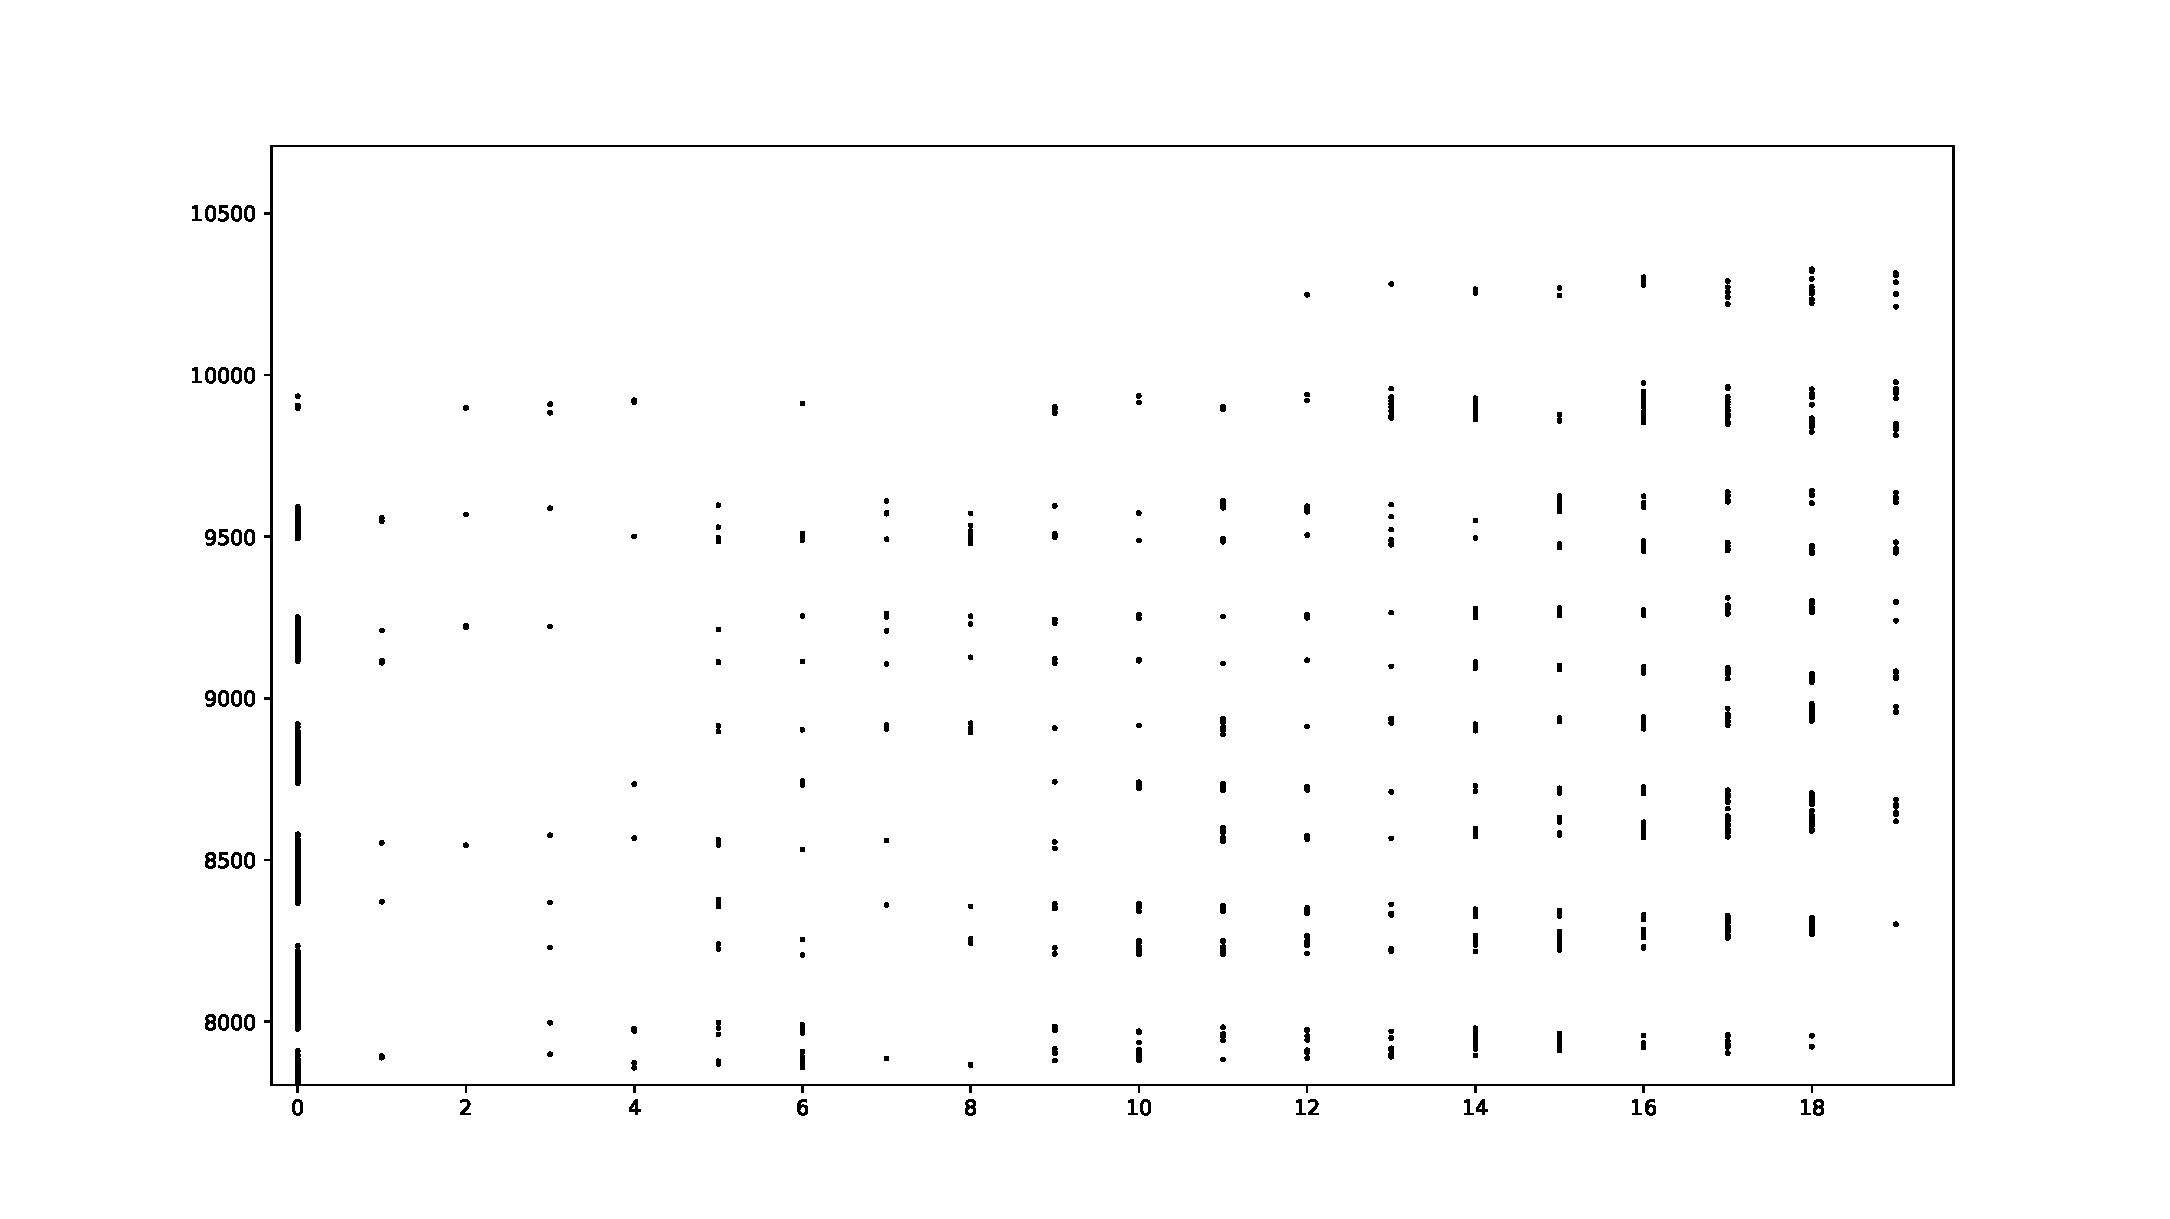
\includegraphics[width=\textwidth]{onv_latency_prev}
    \caption[Latency encoded ONV]{Latency encoding of a subset of photoreceptors from the ONV in Figure~\ref{fig:onv_prev}. Each horizontal line represents the spiking behavior of one photoreceptor, which spikes once in the 20 timestep interval. Excited photoreceptors spike earlier than less excited ones, which spike later.}
    \label{fig:onv_encode_latency}
\end{figure}

Latency encoding focuses on the timing of spikes rather than the spiking frequency. Each neuron is allowed to fire once in the simulated time interval; neurons with higher probabilities of firing emit their spike earlier than neurons with lower probabilities. This encoding method results in sparser inputs to the SNN when compared to rate encoding and, consequently, also makes it difficult for the model to converge.

Figure~\ref{fig:onv_encode_latency} contains spikes that result from latency encoding the ONV from Figure~\ref{fig:onv_prev}. In the figure, we see that very excited neurons fire at the first timestep and partially excited neurons fire sometime afterwards. The spikes at the last timestep represent inputs of 0.0.

%********************************************************************%

\section{Outputs}

A problem associated with using SNNs is related to interpreting the output spike trains. For classification problems, each output neuron is associated with one possible class. The output spike trains are then integrated over a number of timesteps and the output label is that of the neuron with the most spikes, as illustrated in Figure~\ref{fig:snn_classifier}. 

\begin{figure}
    \centering
    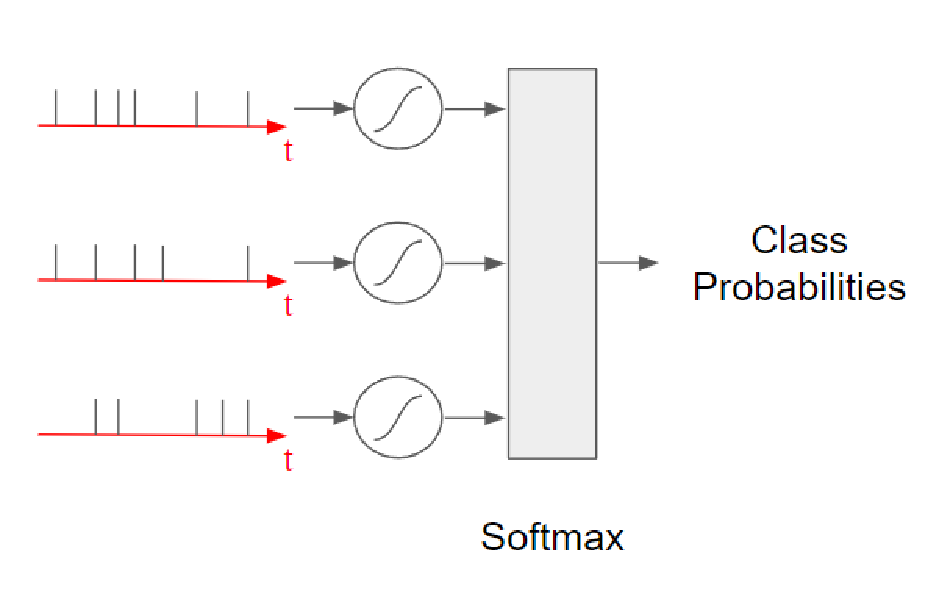
\includegraphics[width=0.5\textwidth]{snn_classifier}
    \caption[Interpreting spike trains to classify inputs]{An example on how spike trains can be interpreted for the purposes of a classification task. Here, each spike train is integrated to count the spikes during a time interval. These counts are then passed to a softmax layer. Each neuron is assigned to a possible class, and the predicted label is that of the neuron with the most spikes.}
    \label{fig:snn_classifier}
\end{figure}

Our application in this thesis, however, takes the form of a regression problem that involves outputting predictions for modifying two gaze angles. Thus far, SNN research has focused on classification as there is no standard way to interpret spikes into floating point values.

To solve this regression problem, we utilize a linear layer to transform outputs from our SNN into the desired angular modifications $\Delta\theta$ and $\Delta\phi$. One option would be to consolidate the output spike train somehow, such as with a sum or average, and then normalize the values. A technique that has not been explored much, but is suggested in the snnTorch package, is to utilize the membrane voltages of the last layer. We pass each neuron's membrane voltage at the last timestep through a linear transformation that outputs our two angular changes. This technique helps with backpropagation learning, as the network can learn what membrane voltages it should target to have at the end of the computation. Note that the network outputs values at each timestep, but our predicted values are the model's outputs at the final timestep.

%%%%%%%%%%%%%%%%%%%%%%%%%%%%%%%%%%%%%%%%%%%%%%%%%%%%%%%%%%%%%%%%%%%%%%

% signals and encoding
% \chapter{Data and Encodings}

%********************************************************************%
% \section{Spiking Inputs}

%%%%%%%%%%%%%%%%%%%%%%%%%%%%%%%%%%%%%%%%%%%%%%%%%%%%%%%%%%%%%%%%%%%%%%

\chapter{The SLiNet Model}

In this chapter, we discuss how the architecture of our foveation DNN is based on that of the LiNet, which was described in Section~\ref{sec:LiNets}.

\section{Architecture}

We base our SNN architecture on the LiNet that was designed for this task by \citep{Masaki_linet}. The existing LiNet DNN has 5 locally-connected layers plus one final fully-connected layer, as illustrated in Figure~\ref{fig:linet_foveation}. Each layer has $1/5$ the number of neurons of the previous layer. 

To build our spiking LiNet, or SLiNet, we start with a 4 layer foveation LiNet and replace the ReLU units with spiking neurons. We retain the fully-connected output layer to transform the membrane voltages into the two gaze angles. Our SLiNet model is summarized in Figure~\ref{fig:linet_arch}. We compare code samples implementing an ANN and an SNN in Figure~\ref{fig:code}.

\begin{figure}
    \centering
    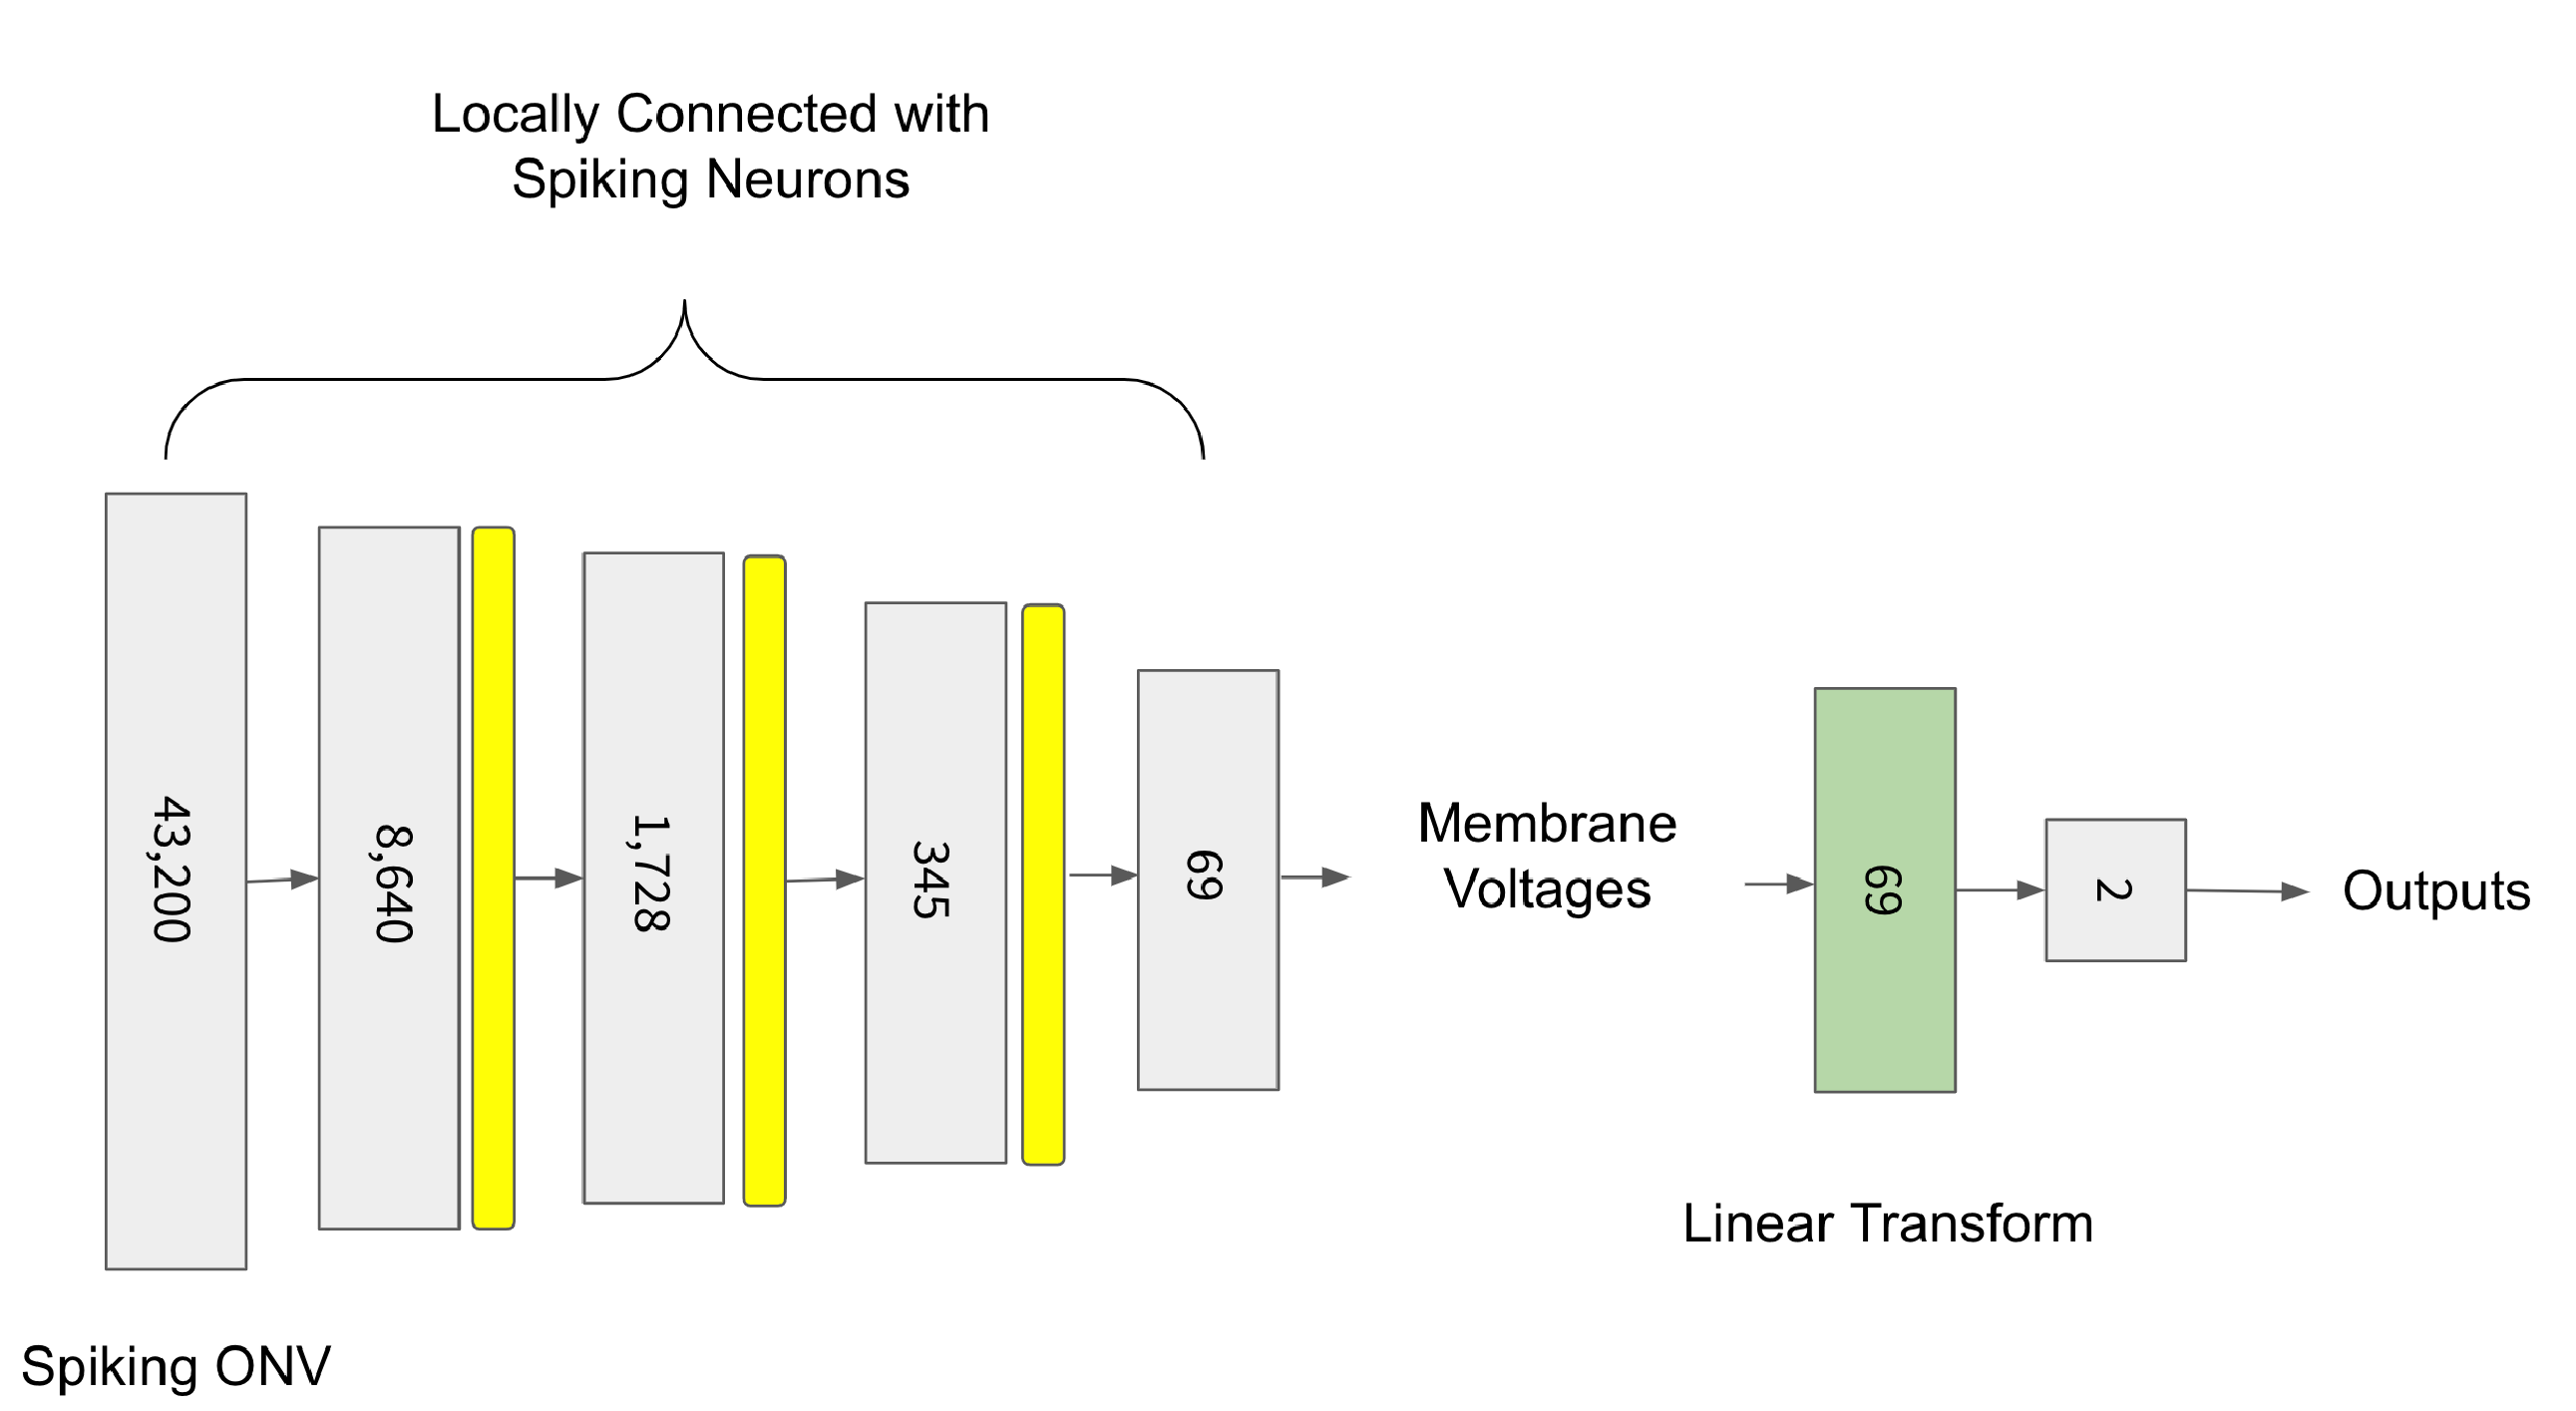
\includegraphics[width=\textwidth]{arch_spiking}
    \caption[SLiNet architecture]{Our spiking foveation LiNet architecture, the SLiNet. The first four layers reflect that of the LiNet, but employ spiking neurons (yellow) rather than the conventional neurons with ReLU activation functions. The fourth layer passes the membrane voltages through a linear transform, which produces an output of dimension two, representing the changes in gaze angles $\Delta\theta$ and $\Delta\phi$.}
    \label{fig:linet_arch}
\end{figure}

% \begin{figure}
%     \centering
%     \lstinputlisting[language=Python, firstline=1, lastline=10, caption={}]{figures/code1.py}
%     \caption[]{Normal feedforward network.}
%     \label{fig:code_ann}
% \end{figure}

% \begin{figure}
%     \centering
% \lstinputlisting[language=Python, firstline=13, lastline=31, caption={}]{figures/code1.py}
%     \caption[]{SNN feedforward network. Differences from Figure~\ref{fig:code_ann} include the use of spiking neurons, time-varying input, and the use of a linear layer which transforms membrane voltages from the last layer. }
%     \label{fig:code_snn}
% \end{figure}

\begin{figure}
    \centering
    \begin{subfigure}{0.40\textwidth}
        \centering
        % 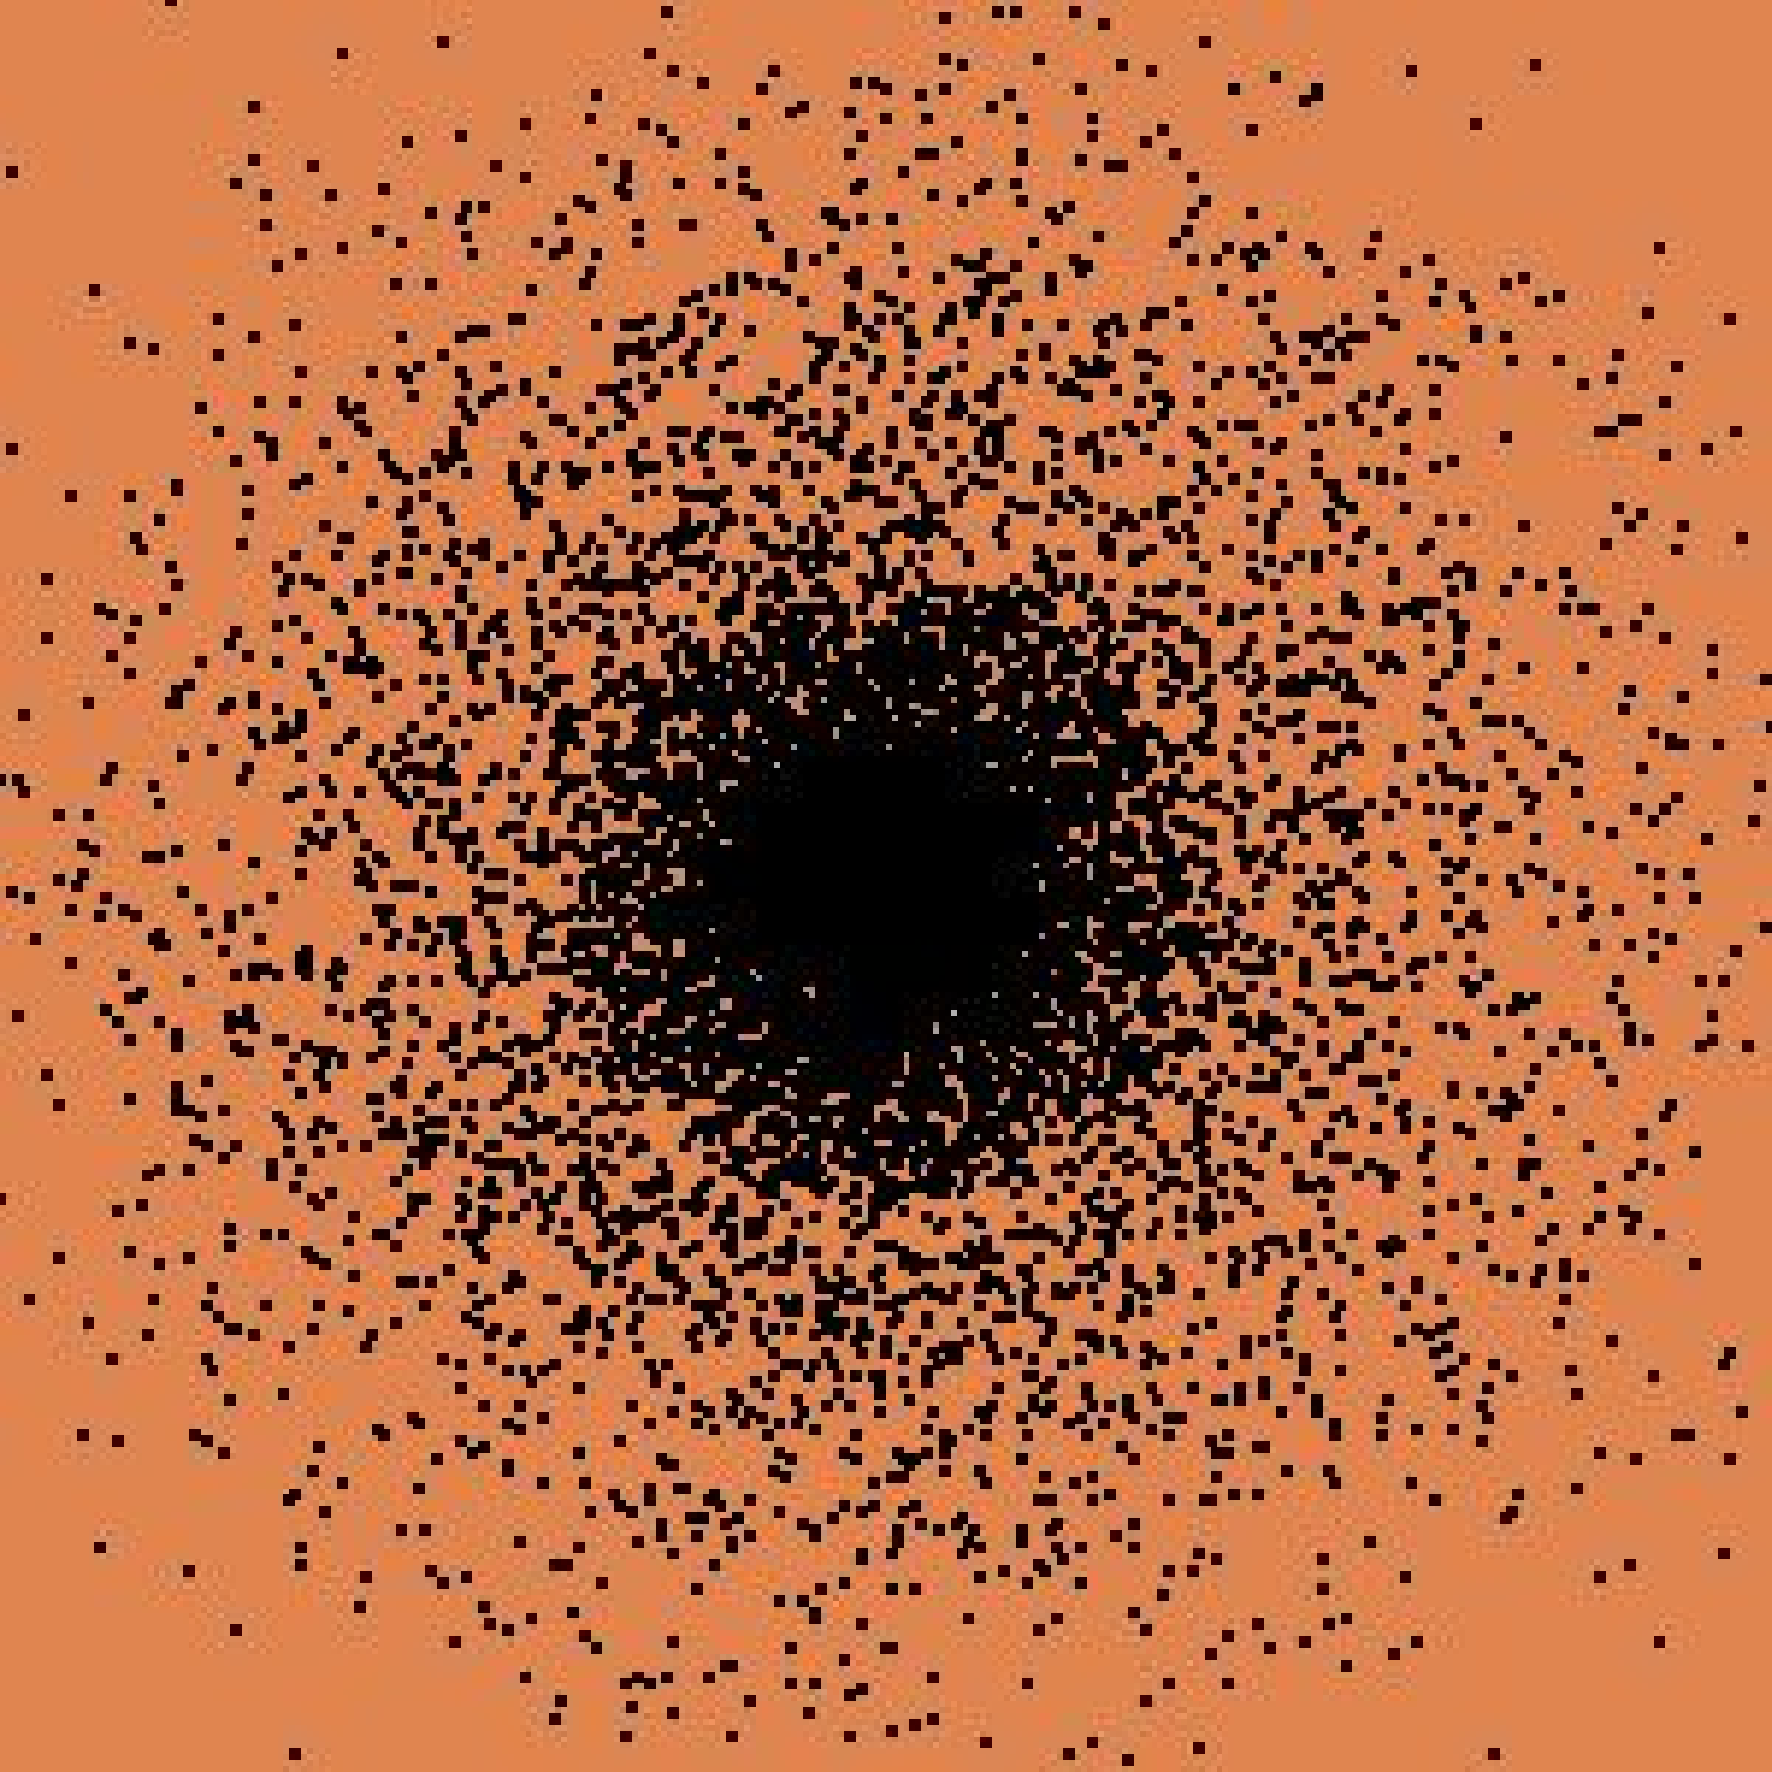
\includegraphics[width=\textwidth]{fixation2}
        \lstinputlisting[language=Python, firstline=1, lastline=10, caption={}]{figures/code1.py}
        \caption{}
    \end{subfigure}
    \hfill
    \centering
    \begin{subfigure}{0.50\textwidth}
        \centering
        % 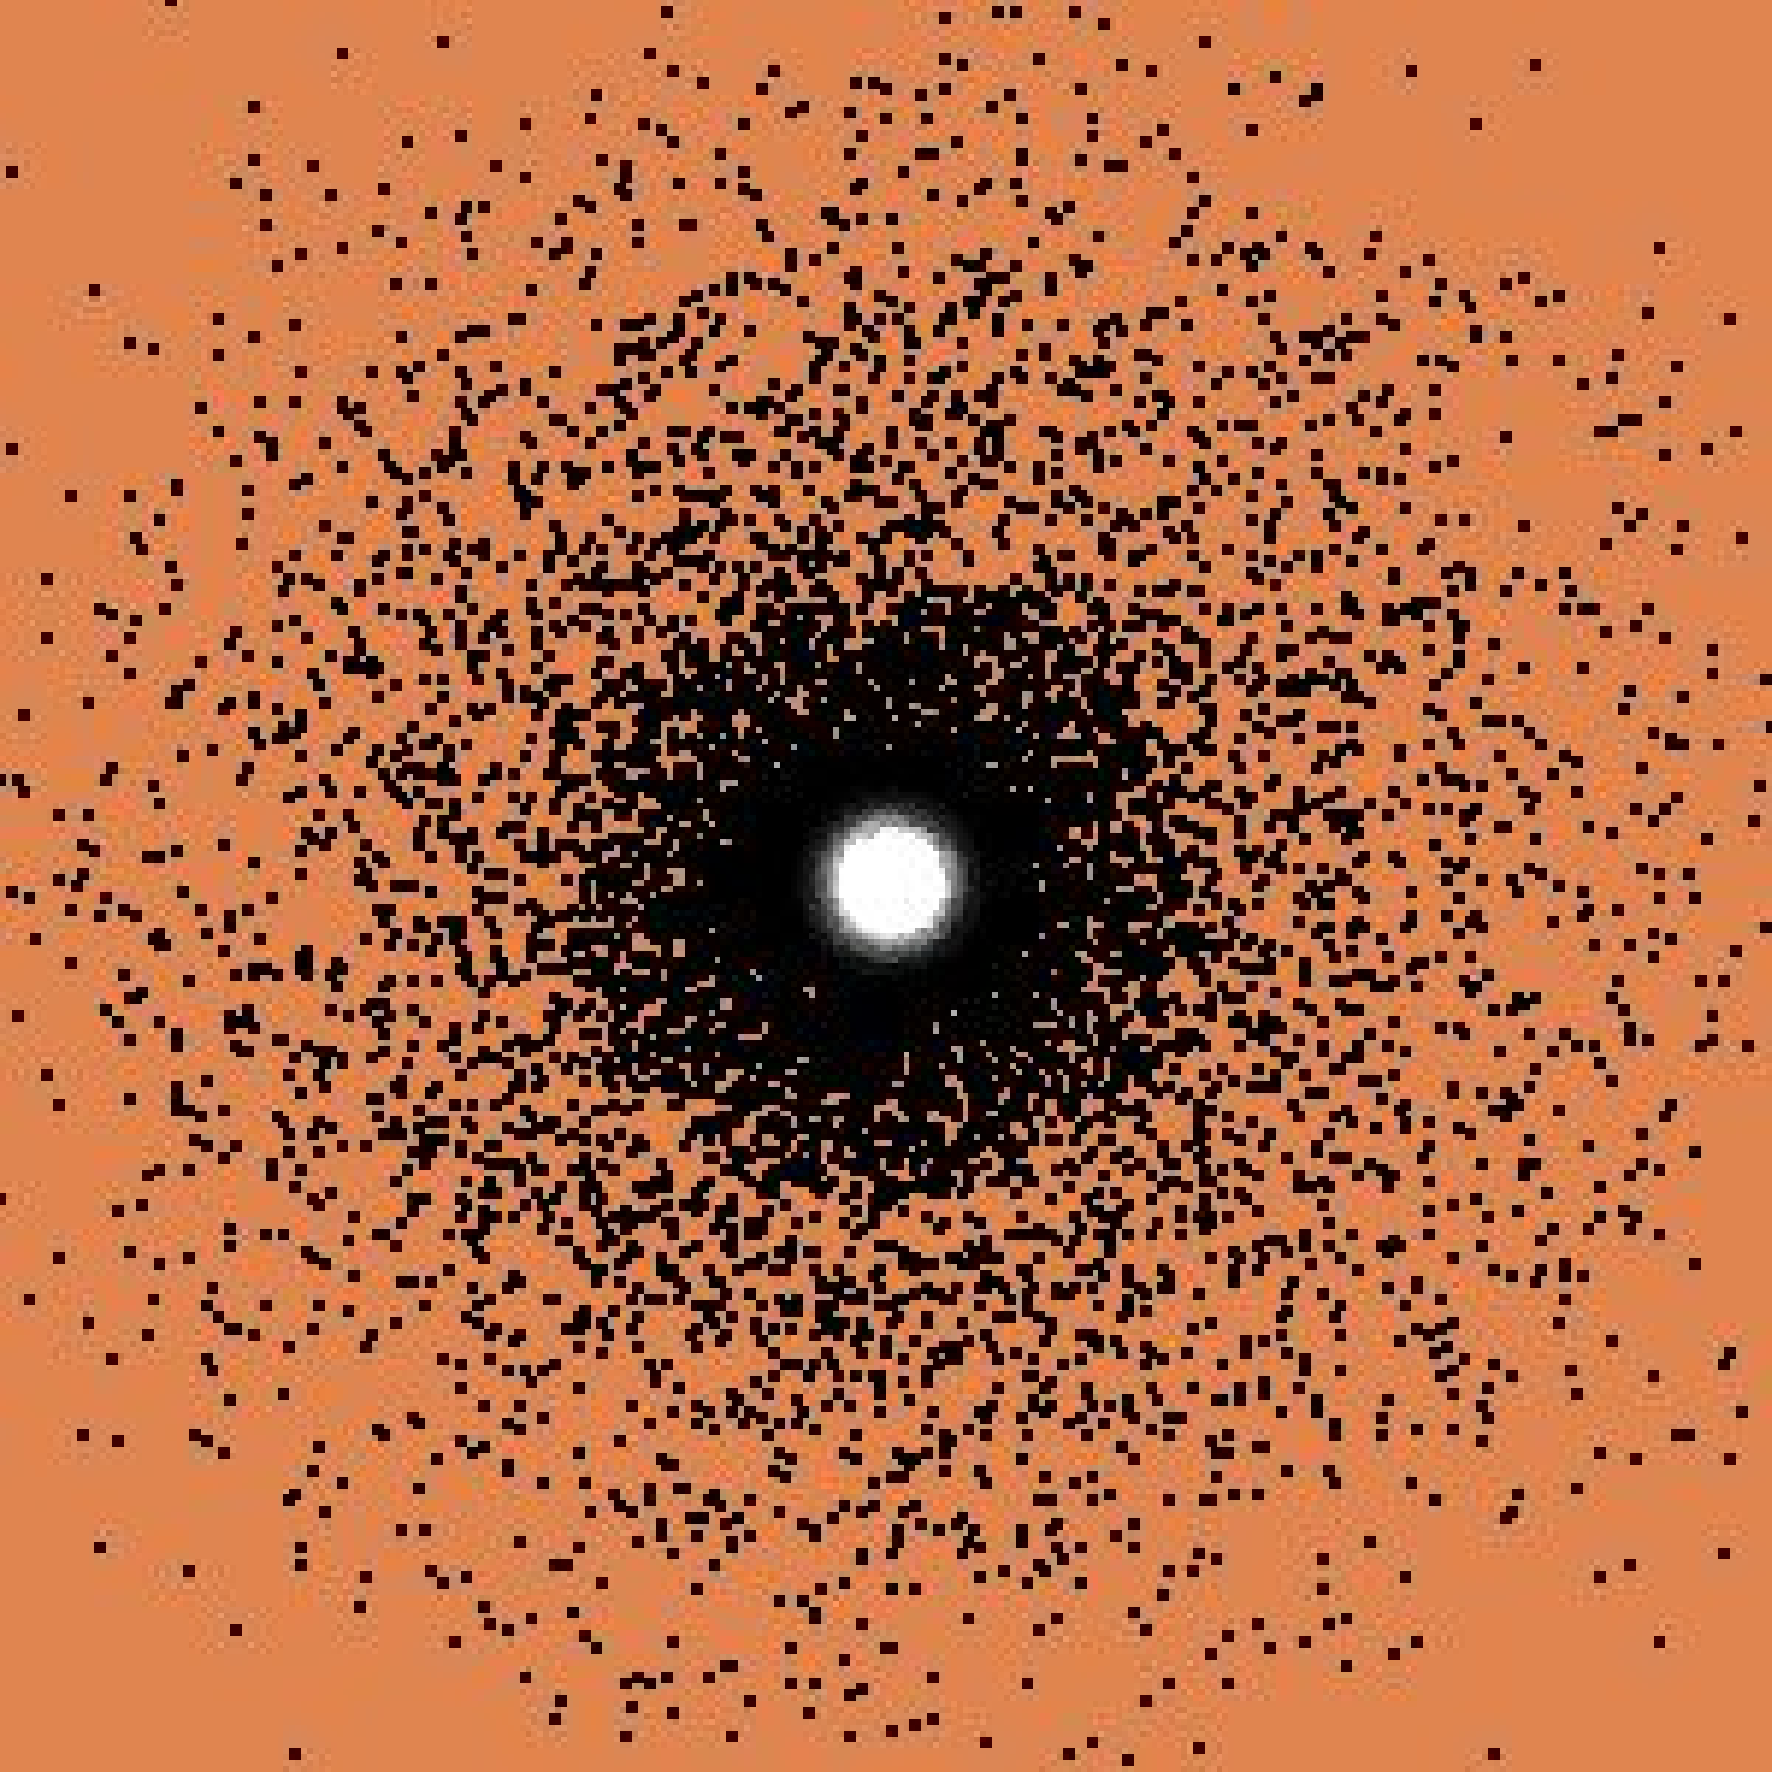
\includegraphics[width=\textwidth]{fixation3}
        \lstinputlisting[language=Python, firstline=12, lastline=30, caption={}]{figures/code1.py}
        \caption{}
    \end{subfigure}
    \caption[Code comparison between a fully-connected ANN and SNN]{Code comparison between a fully-connected ANN (a) and SNN (b). Differences in (b) include the addition of spiking neurons, time-varying input, and the use of a linear transform that transforms membrane voltages from the last spiking layer. Note that ``lif'' is a layer of spiking neurons and that ``fc'' is a fully connected layer. A LIF neuron outputs a tuple with two values: a spike (or a lack thereof) and the current membrane voltage. }
    \label{fig:code}
\end{figure}

% Hybrid model
% \begin{figure}
%     \centering
%     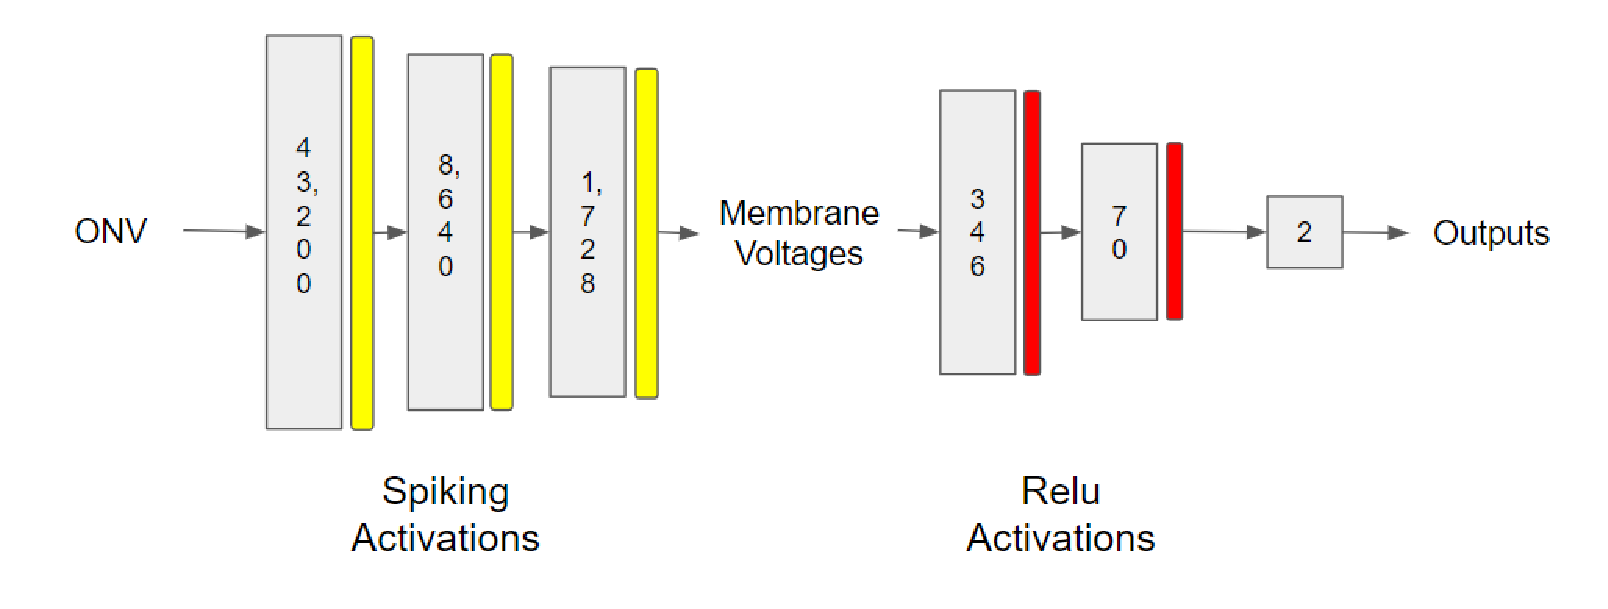
\includegraphics[width=\textwidth]{arch_hybrid}
%     \caption[Hybrid SNN architecture]{Our Hybrid Spiking LiNet architecture.}
%     \label{fig:hybrid_arch}
% \end{figure}

% We were also curious to see the effects of using ReLU activations with spiking activations. We call these models ``hybrid SNNs.'' The architecture has 5 locally connected layers where the first n layers have spiking inputs and the last few use ReLU. There is still one fully connected output layer. The spiking layers compute for a certain number of timesteps and then pass their membrane voltages to the artificial neuron half. This architecture is summarized in Figure~\ref{fig:hybrid_arch}, with a code example shown in Listing~\ref{listing:hybrid_forward}.

% code comparison between ANN, SNN, and Hybrid
% \noindent\begin{minipage}{.45\textwidth}
% \lstinputlisting[label={listing:ann_forward},language=Python, firstline=1, lastline=12, caption={Normal feedforward network.}]{figures/code1.py}
% \end{minipage}\hfill
% \begin{minipage}{.45\textwidth}
% \lstinputlisting[label={listing:snn_forward},language=Python, firstline=15, lastline=35, caption={SNN feedforward network. Differences from listing \ref{listing:ann_forward} include the use of spiking neurons, time-varying input, and the use of a linear layer which transforms membrane voltages from teh last layer. }]{figures/code1.py}
% \end{minipage}

% \lstinputlisting[label={listing:hybrid_forward}, language=Python, firstline=37, lastline=59, caption=A hybrid SNN that hands off the membrane voltages from its final spiking layer to linear layers that use the ReLU activation function.]{figures/code1.py}

% We noticed that adding spiking layers increases noise in the output. With this model, one can make a decision to use a certain number of layers to tradeoff between power usage/latency and accuracy. It also makes computation easier; one can imagine a neuromorphic chip finishing it computation and handing off the result to traditional GPU cores to finish inference. This method only uses the more expensive GPU cores for inference on a lower dimensional vector.

%********************************************************************%

\section{Training}

Here we go over the various decisions made while training our SLiNets.

Our training data set consists of 22.5k data points. We use 20k to create a training set and set aside 2.5k for validation. We do not create a testing set as we evaluate our work through the simulation of the eye model. The data points are collected from the eye model itself. It is kept in a fixed position, looking forward. The ball visual target is moved to random points in the field of view, and the corresponding ONVs are collected. The labels are the angular displacement between the eye's current gaze direction and the direction of the ball in the field of view. To create our D-ONV data set, we simply subtract each ONV from the previous one.

For the LiNet, we use a factor $f$ of 5, meaning each subsequent layer has one-fifth the number of neurons as the previous layer. A number was not reported for $k$, the number of inputs combined at each neuron. We conducted a hyperparameter sweep and use a value of 25. We re-trained the LiNet since we did not have access to the previously trained model. Training was done with a batch size of 16 and a learning rate of 0.001. No regularization was added to the model, and the weights were initialized with He initialization. 
The same hyperparameter values are used when training our SLiNet.

We train our models for around 100 epochs, which is about when the loss values start to plateau. We plot the training and validation losses for both a 5-layer LiNet and our 4-layer SLiNet. Figure~\ref{fig:loss_normal} shows plots for each model trained with the ONV and Figure~\ref{fig:loss_delta} shows plots for each model trained with the D-ONV. In both plots we can see that the LiNet achieves loss values one order of magnitude smaller than the spiking models. However, the spiking models still converge to low-loss values. The LiNet validation loss is much higher when using the D-ONV, which may indicate that it will have trouble generalizing to our test scenarios.
% We can see the effect of including a ReLU activated layer in the hybrid model as it has slightly lower training and validation loss than the SLiNet achieves. 

% Again the Hybrid SLiNet architecture achieves slightly lower loss values than the pure SLiNet architecture's loss values.

\begin{figure}
    \centering
    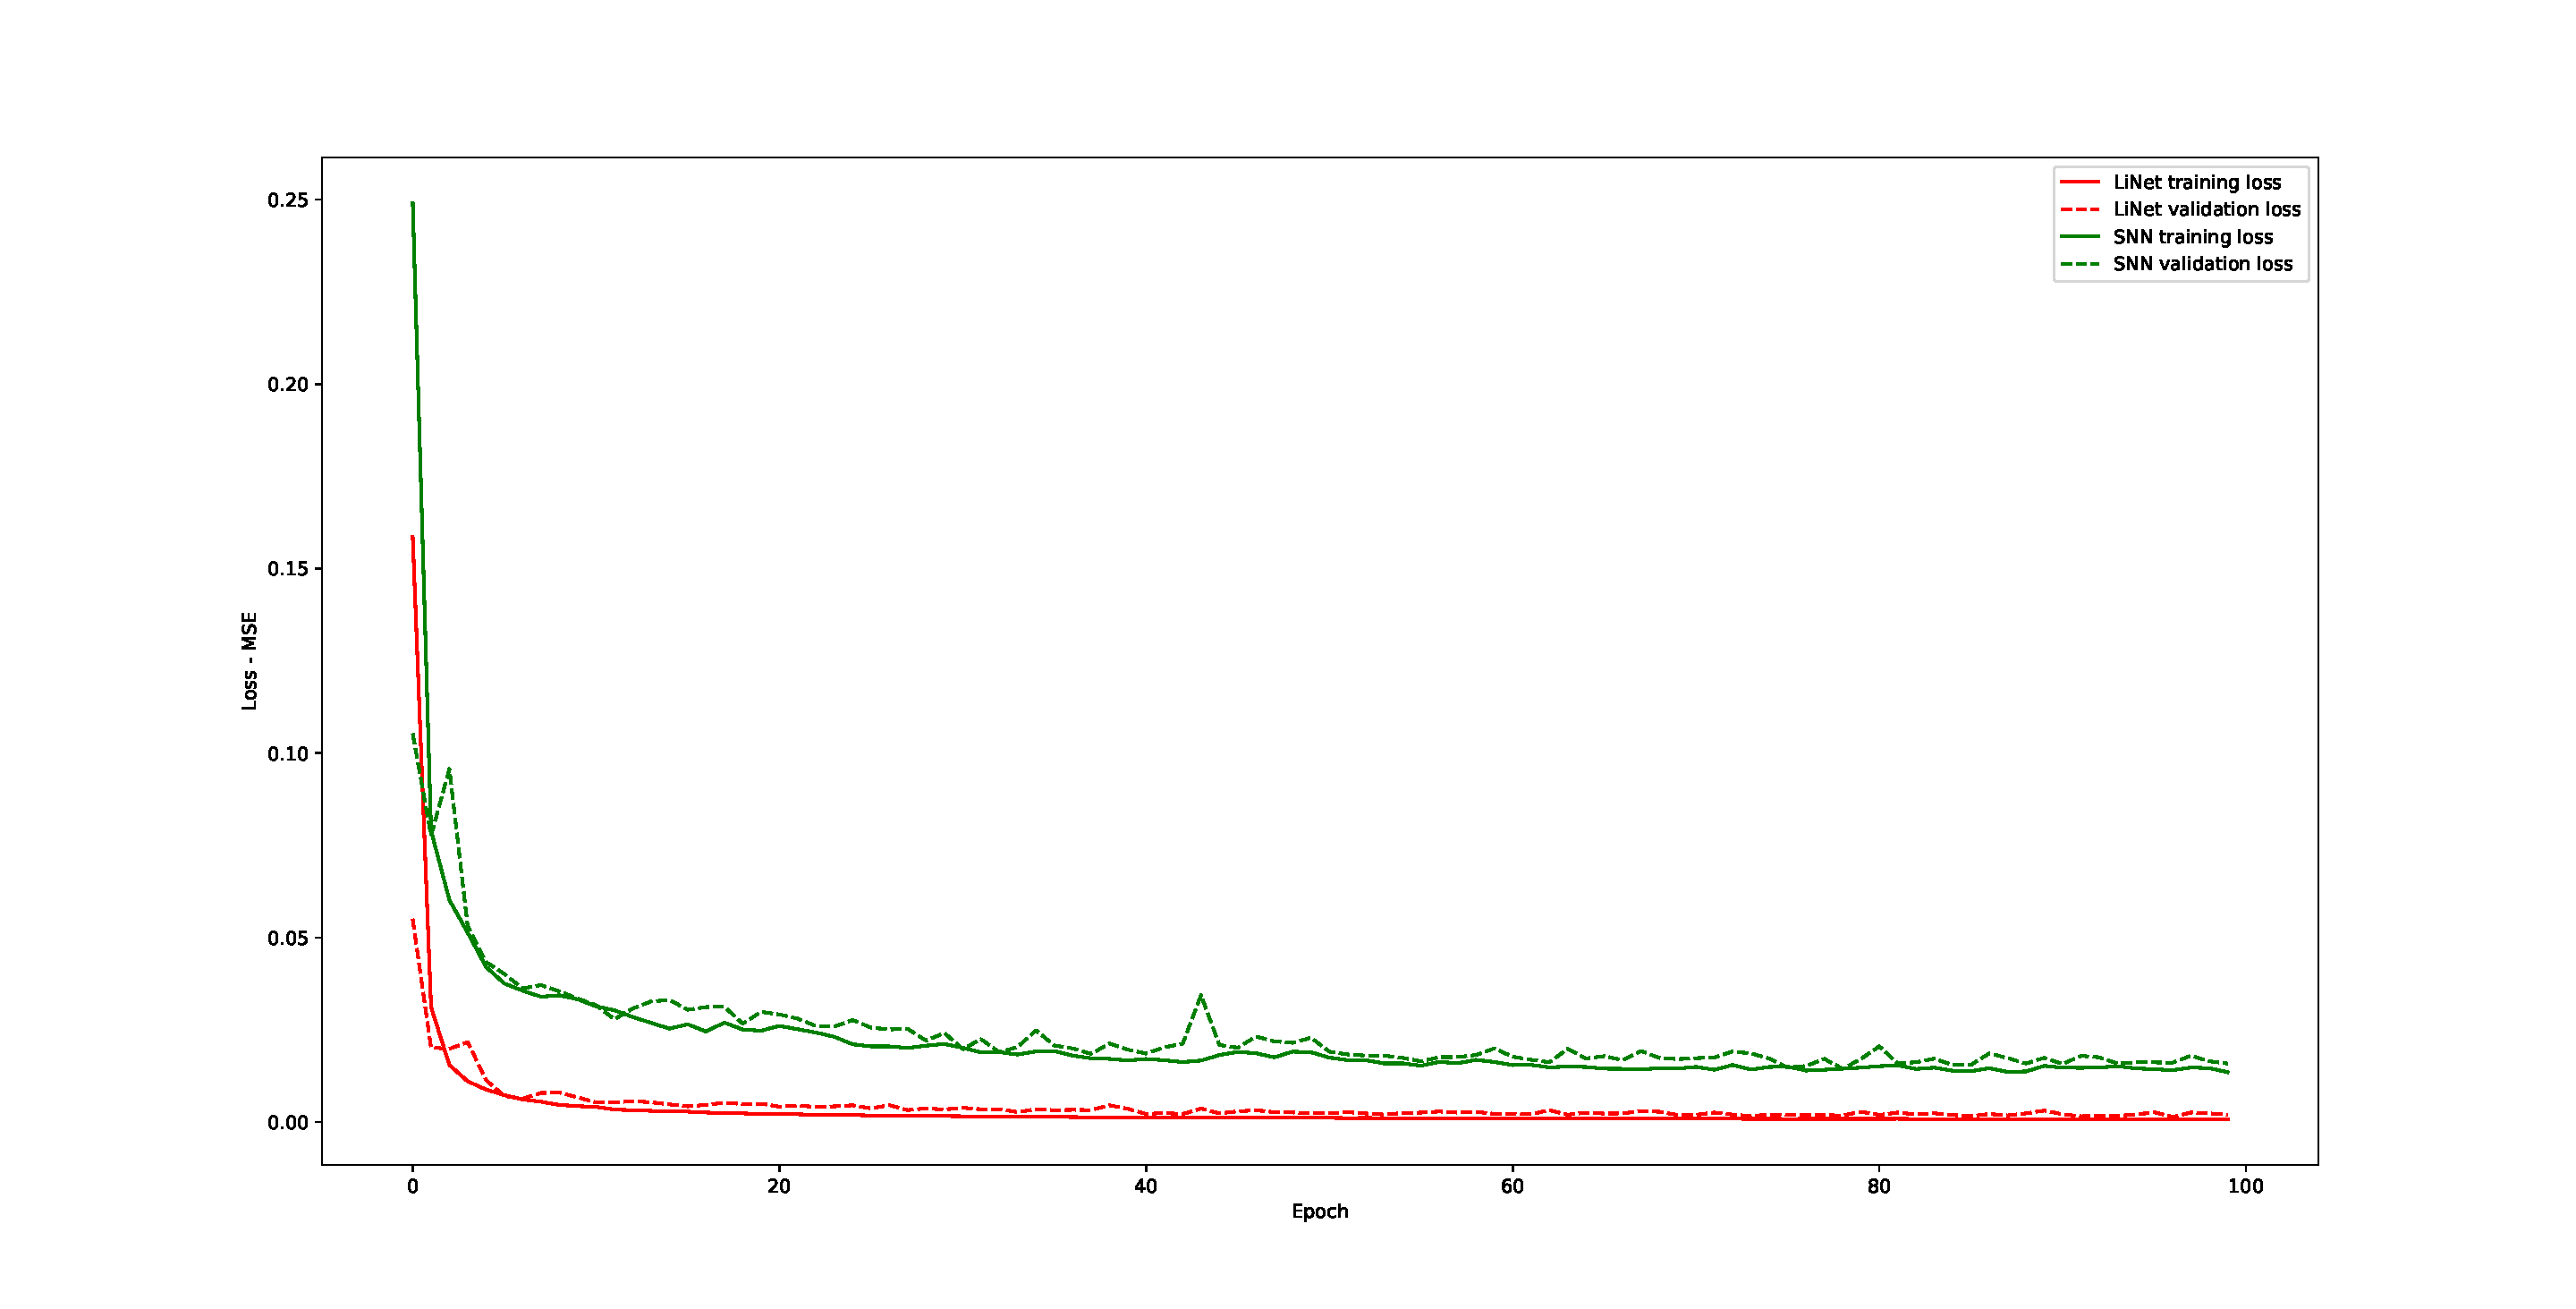
\includegraphics[width=\textwidth]{loss_normal}
    \caption[Training and validation loss using ONVs]{The LiNet converges very quickly and achieves very low loss values. There is no indication of overfitting from either model as the validation losses continue to decrease with the training losses.}
    \label{fig:loss_normal}
\end{figure}

\begin{figure}
    \centering
    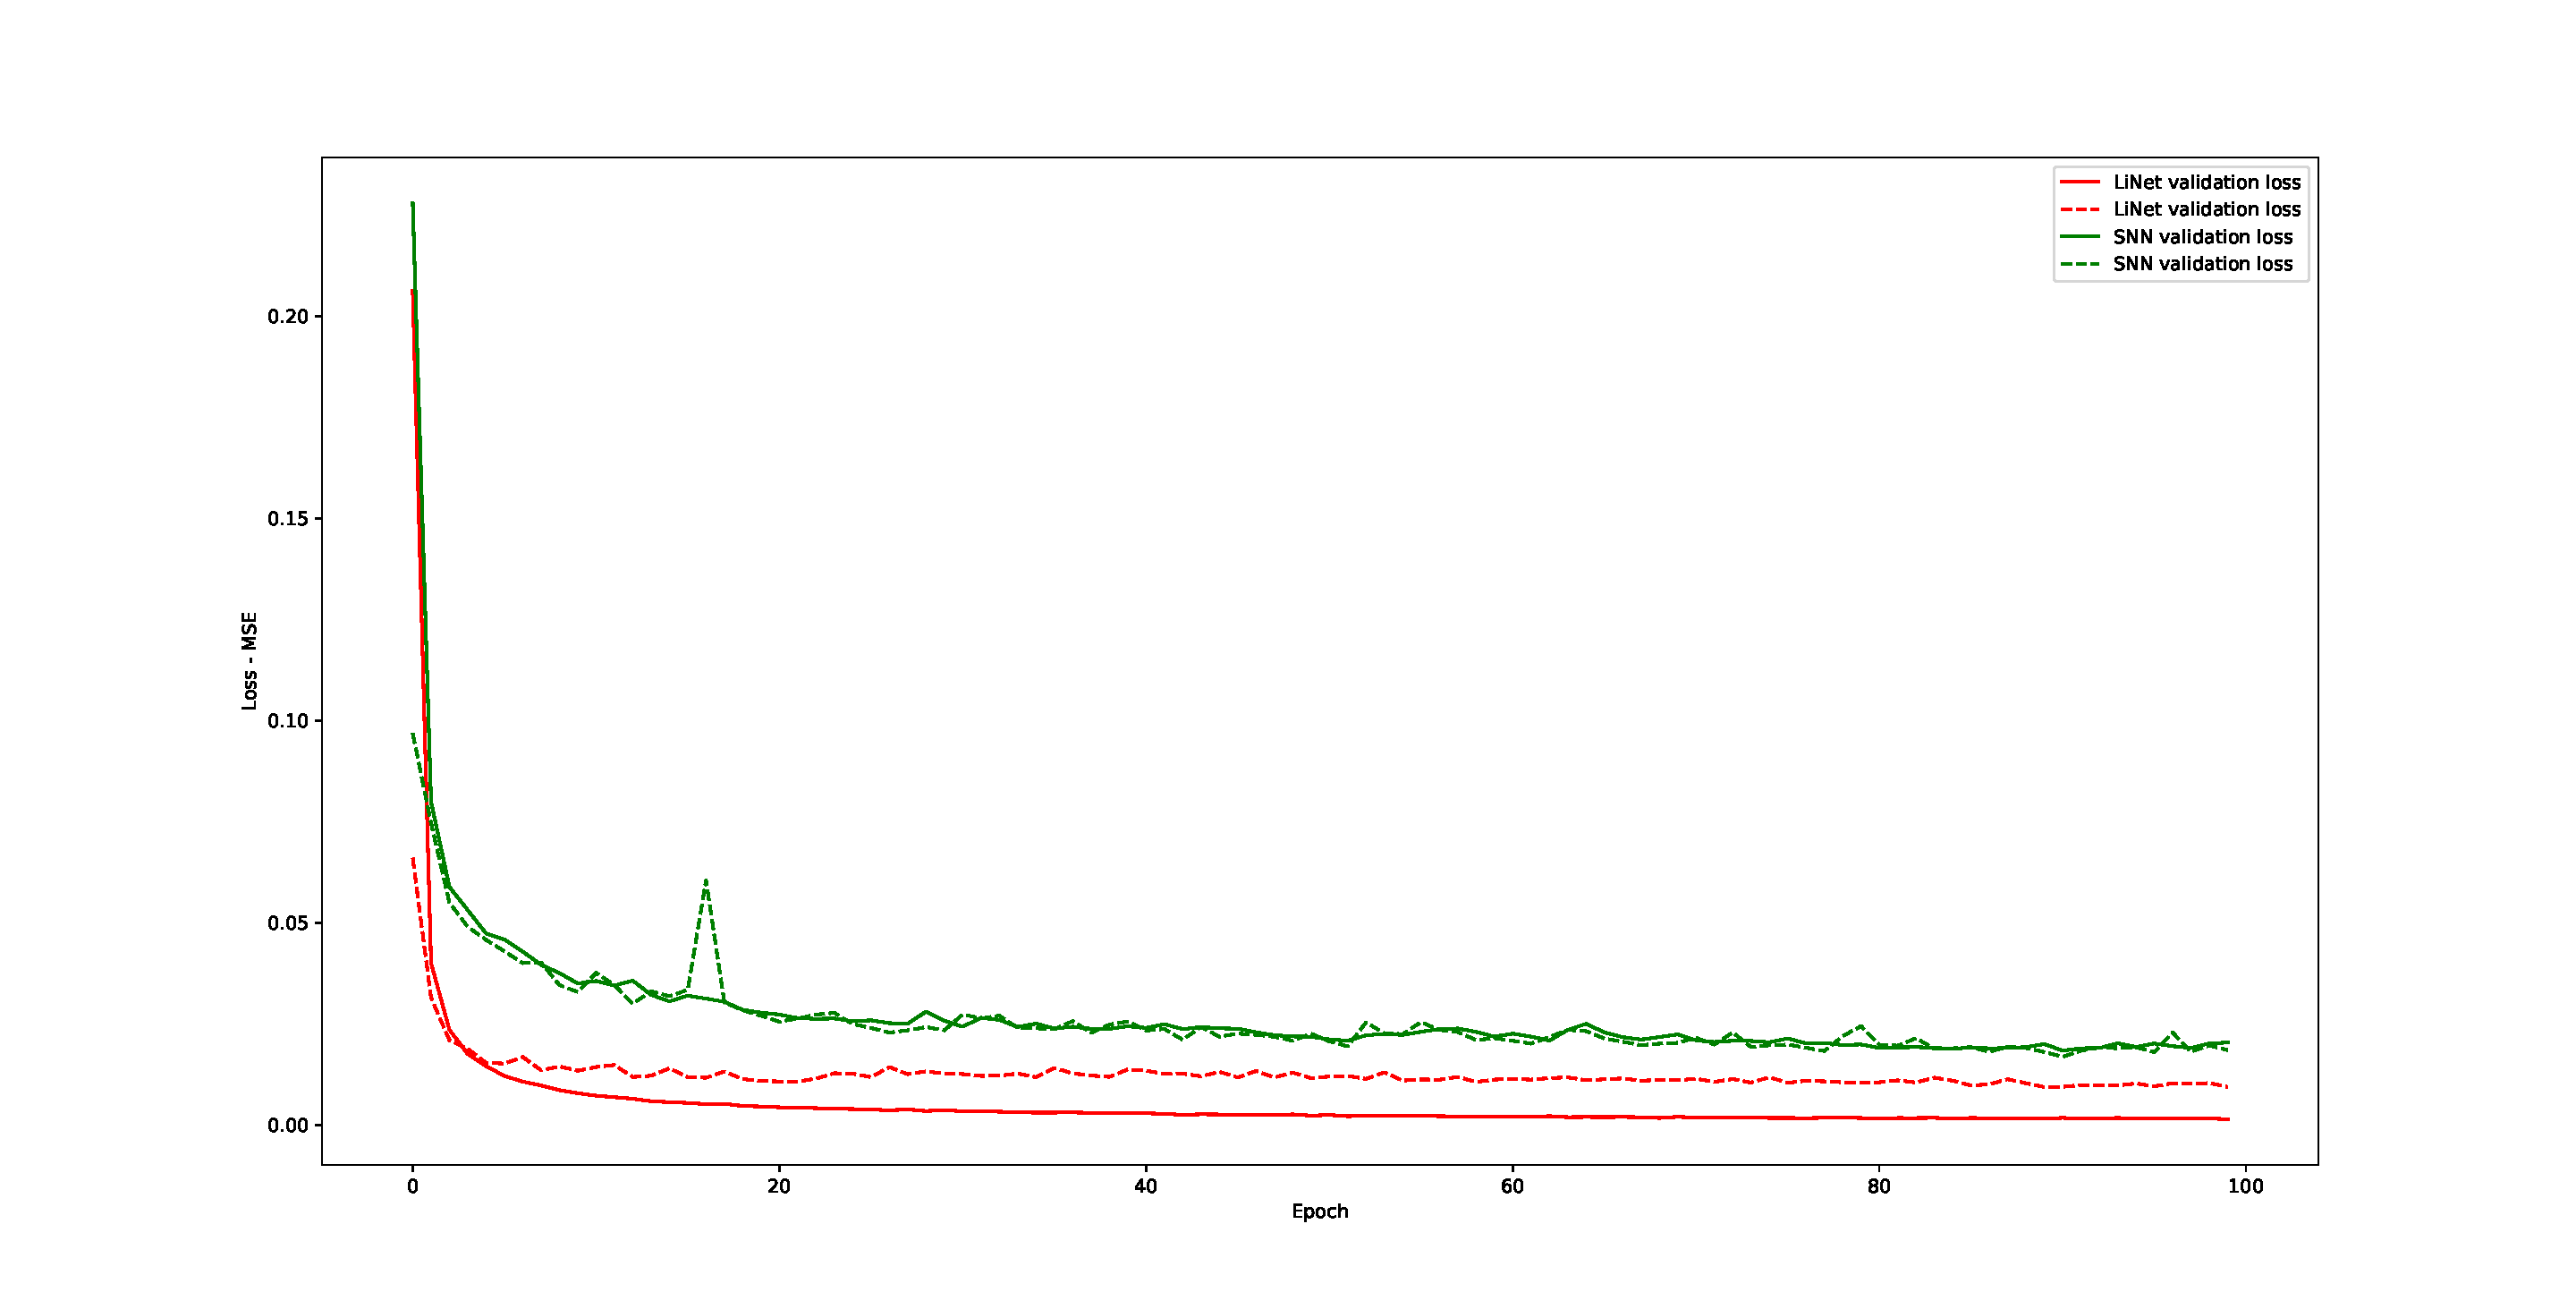
\includegraphics[width=\textwidth]{loss_delta}
    \caption[Training and validation loss using D-ONVs]{When using the D-ONV, the LiNet again converges quickly, but has high validation loss, whereas our SLiNet still converges to reasonably low loss values.}
    \label{fig:loss_delta}
\end{figure}

We treat $\beta$ as a hyperparameter, although it can also be trained in different ways. We choose not to tune it on a per-layer or individual neuron basis with backpropagation. However, we do treat the threshold voltage for each neuron as a trainable parameter. By default, all neuron thresholds are set to 1.0, but we find that randomly initializing these thresholds to values in the range $[0,1]$ yields the best results.

When a neuron outputs a spike, we can either reset the membrane voltage to zero or subtract the threshold voltage from the current membrane voltage. We refer to these options as ``reset'' and ``subtract,'' respectively. With the subtract method, the neuron will have a non-zero membrane voltage if it had accumulated a large amount of voltage before the spike. On the other hand, the resetting method results in sparser spiking and potential energy savings, but it presents a bigger challenge to learning as it is more lossy. We use the subtraction method in our neurons.

\subsection{Number of Timesteps}

The length of the spiking input, otherwise referred to as the number of timesteps, is a hyperparameter of our SLiNet. This hyperparameter determines how many timesteps each neuron is afforded to accumulate voltage and emit spikes. More timesteps allow more downstream neurons to fire, which may help computation, but will also consume more energy to run. Conversely, models using a lower number of timesteps may train quickly, but they will have difficulty converging to a low enough loss value. The typical number of timesteps ranges from the hundreds to thousands. After conducting a hyperparameter sweep, we empirically found that 20 timesteps was enough for our model to converge. Higher numbers of steps were more difficult to train and did not seem to affect performance.

% this is odd, have graphs of loss for various timesteps?

\subsection{Surrogate Gradients}

On the backpropagation pass, we encounter the Heaviside step function through our spiking activation function. Its local derivative is 0 everywhere except for the time of the spike, where it is infinite. This is the main barrier to deep learning with spiking neural networks, as our gradient will either become 0 or infinity after reaching this function on the backward pass. snnTorch handles this by passing through the gradient when there is a spike and 0 when there is not. This enables some learning, but is not good enough for our task. We experimented with surrogate gradients, which are functions that approximate the Heaviside step function but are differentiable everywhere \citep{surrogate_grad}. The spiking activation is still used in the forward pass, but the surrogate gradient is used on the backward pass.

% math of backprop with step func?

The approximation of choice is the fast sigmoid function, so named as it is faster to compute than the standard sigmoid function. The function and its derivative are plotted in Figure~\ref{fig:surrogate_grad}. We find that our model fails to converge without the use of a surrogate gradient.

% figure of sigmoid and its derivative
\begin{figure}
    \centering
    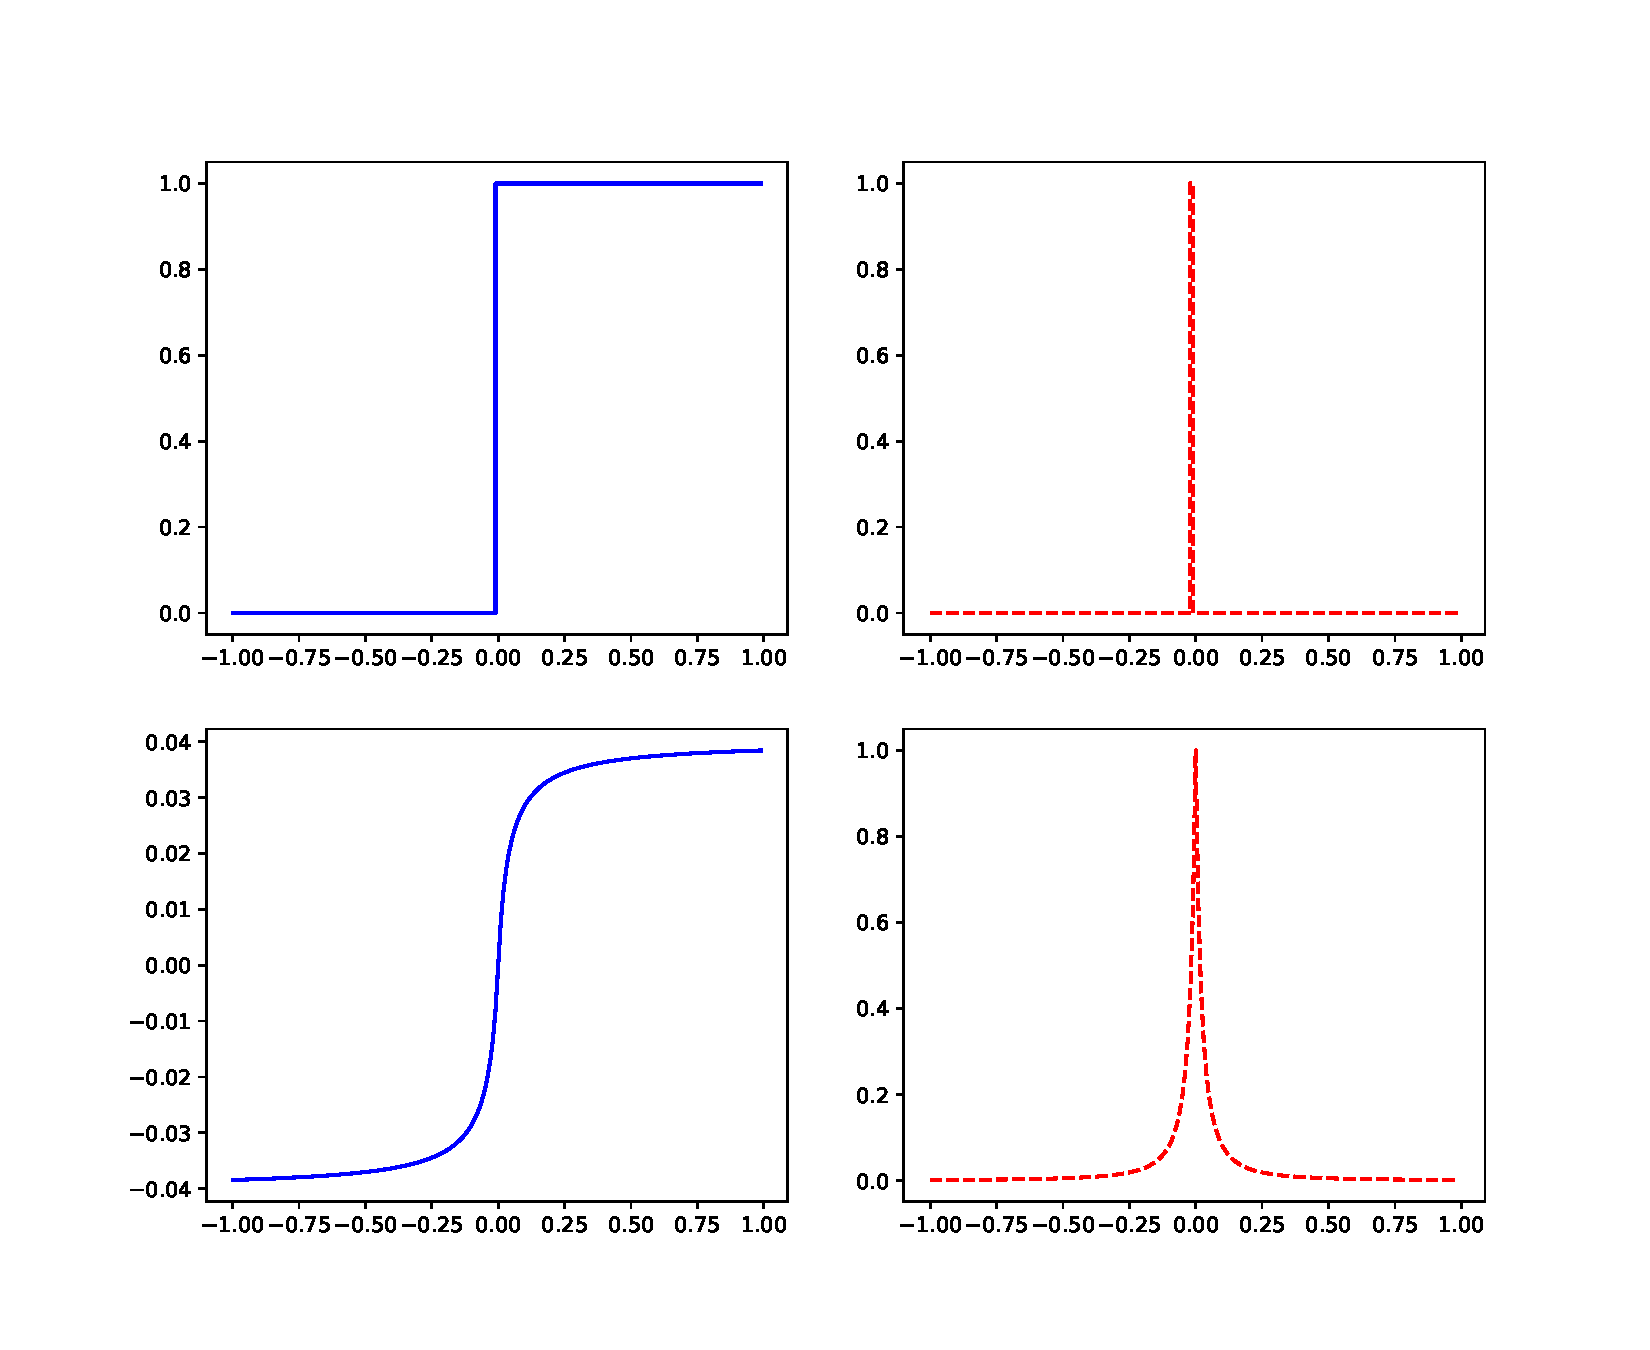
\includegraphics[width=0.8\textwidth]{surrogate_grad}
    \caption[Derivatives of the Heaviside step and fast sigmoid functions]{We compare the Heaviside step and fast sigmoid functions (blue) and their derivatives (red). The derivative of the Heaviside step function is 0 everywhere except at the location of the threshold, where it is infinity. This is problematic during backpropagation, where the derivative will either be set to zero or explode. By contrast, the derivative of the fast sigmoid function is smooth and allows gradients to flow through the neuron. }
    \label{fig:surrogate_grad}
\end{figure}

\subsection{Loss Calculation}

The SLiNet computation graph can be unrolled exactly like a recurrent neural network (RNN), so backpropagation through time (BPTT) is used during training. Specifics of the unrolled computation graph can be found in Figure~\ref{fig:snn_loop_unroll}. The SLiNet can also be encouraged to reach correct outputs at earlier timesteps by collecting the output from each timestep, calculating the loss at each timestep, and summing all of these losses together. This unfortunately requires more memory than our GPU has capacity for, so we could not experiment with this method. Because our model required a relatively low number of timesteps to run, we utilized BPTT and looked back through all 20 timesteps.

%********************************************************************%

\section{On Converting an ANN}

The ideas from this chapter are relevant only if one is training a SLiNet from scratch, which is the approach taken in this thesis. However, we did want to compare the performance of our trained SLiNet to that of one converted from an ANN. Inspired by \citet{rathi2020enabling}, we tried an approach where we first scaled the weights and biases as an initialization step. We then trained this model on the data using the fast sigmoid surrogate gradient. Unfortunately, this model failed to converge. Hence, we cannot report on differences between training and converting a SLiNet on our object tracking task.

%%%%%%%%%%%%%%%%%%%%%%%%%%%%%%%%%%%%%%%%%%%%%%%%%%%%%%%%%%%%%%%%%%%%%%

\chapter{Experiments and Results}

We test the operation of our foveation SLiNet in two ways. First, we move the target in three different trajectories and observe if the eye can track it. Second, we use data collected from human subjects to see if the eye movements resulting from the use of our SLiNet are realistic. Both types of tests are used in the work of \citet{Masaki}. 

We compare results using both the ONV and the D-ONV, with LiNet performance treated as a baseline. In each subsection, we plot the angular displacement of the ball with a black line and compare that to the movement generated by our 4-layer SLiNet (blue line) and a 5-layer LiNet (orange line).

%********************************************************************%
\section{Movements}
%********************************************************************%

\subsection{Fixation}

This test does not involve any movement of the target. We keep the target fixed in a location directly in front of the eye and observe how well it is kept fixated in the foveal region of the retina. An unrealistic model would fixate perfectly on the ball and not move, whereas a more realistic model allows the target to drift around the foveal region. These small movements are similar to micro-saccades in human eyes where a movement in one direction is balanced with a consecutive movement in the opposite direction. Figure~\ref{fig:fixation} shows this type of movement generated from the use of our SLiNet using the D-ONV across four timesteps.

% TODO: describe figure more
% can't see movement easily
\begin{figure}
    \centering
    \begin{subfigure}{0.20\textwidth}
        \centering
        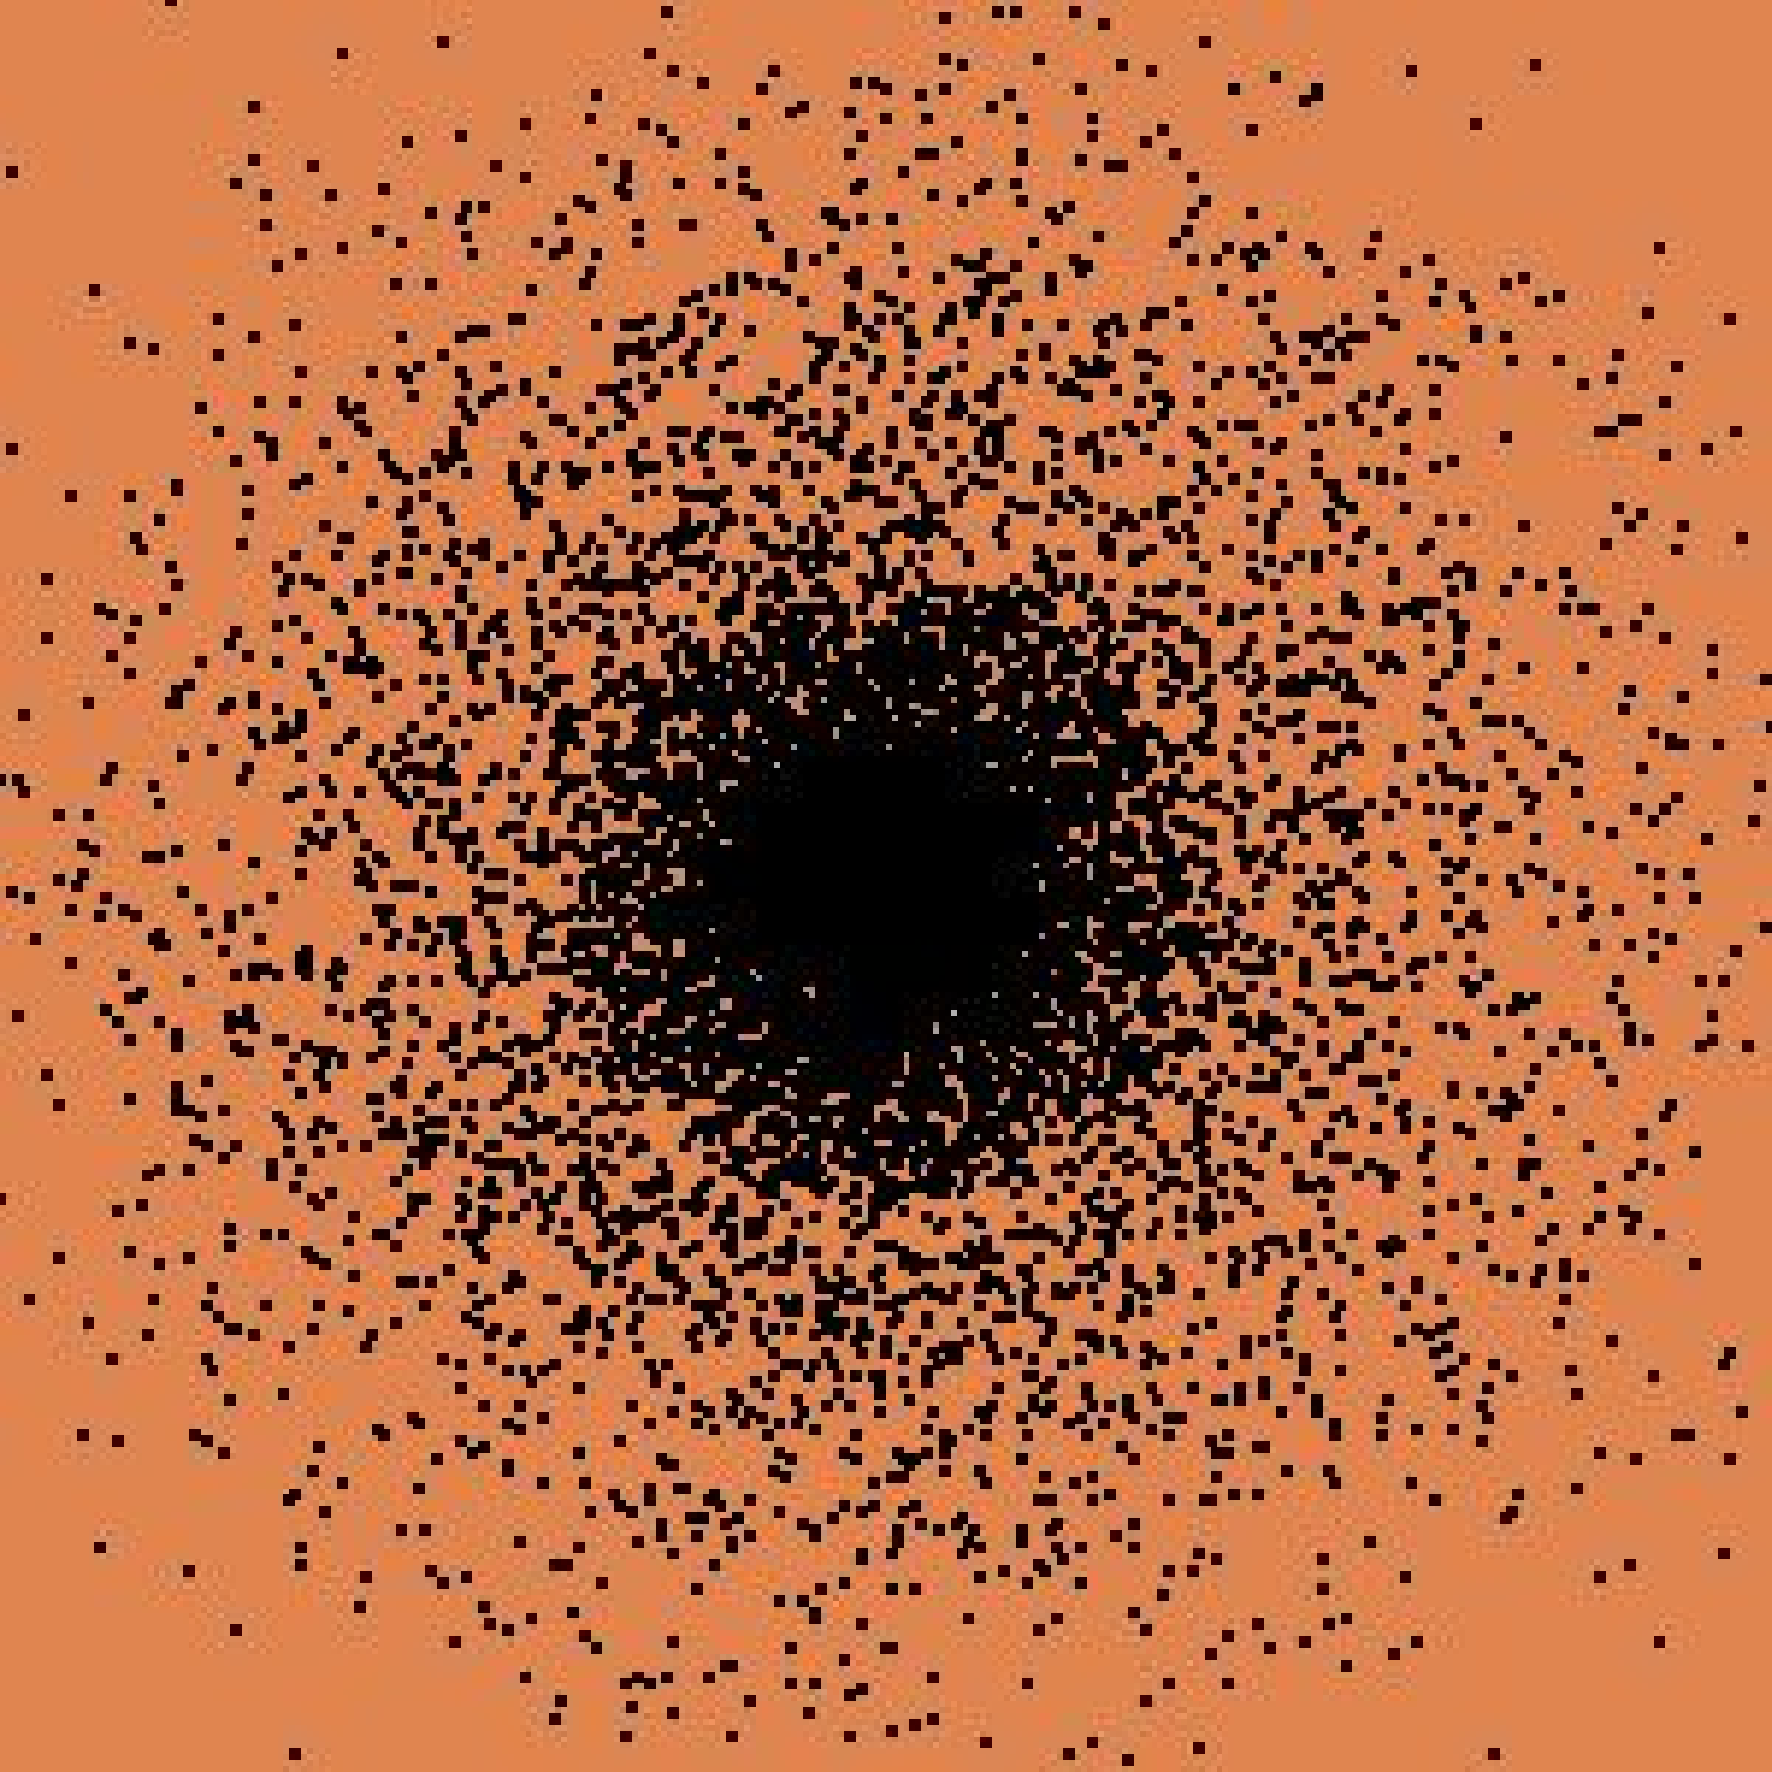
\includegraphics[width=\textwidth]{fixation2}
        \caption{}
    \end{subfigure}
    \hfill
    \centering
    \begin{subfigure}{0.20\textwidth}
        \centering
        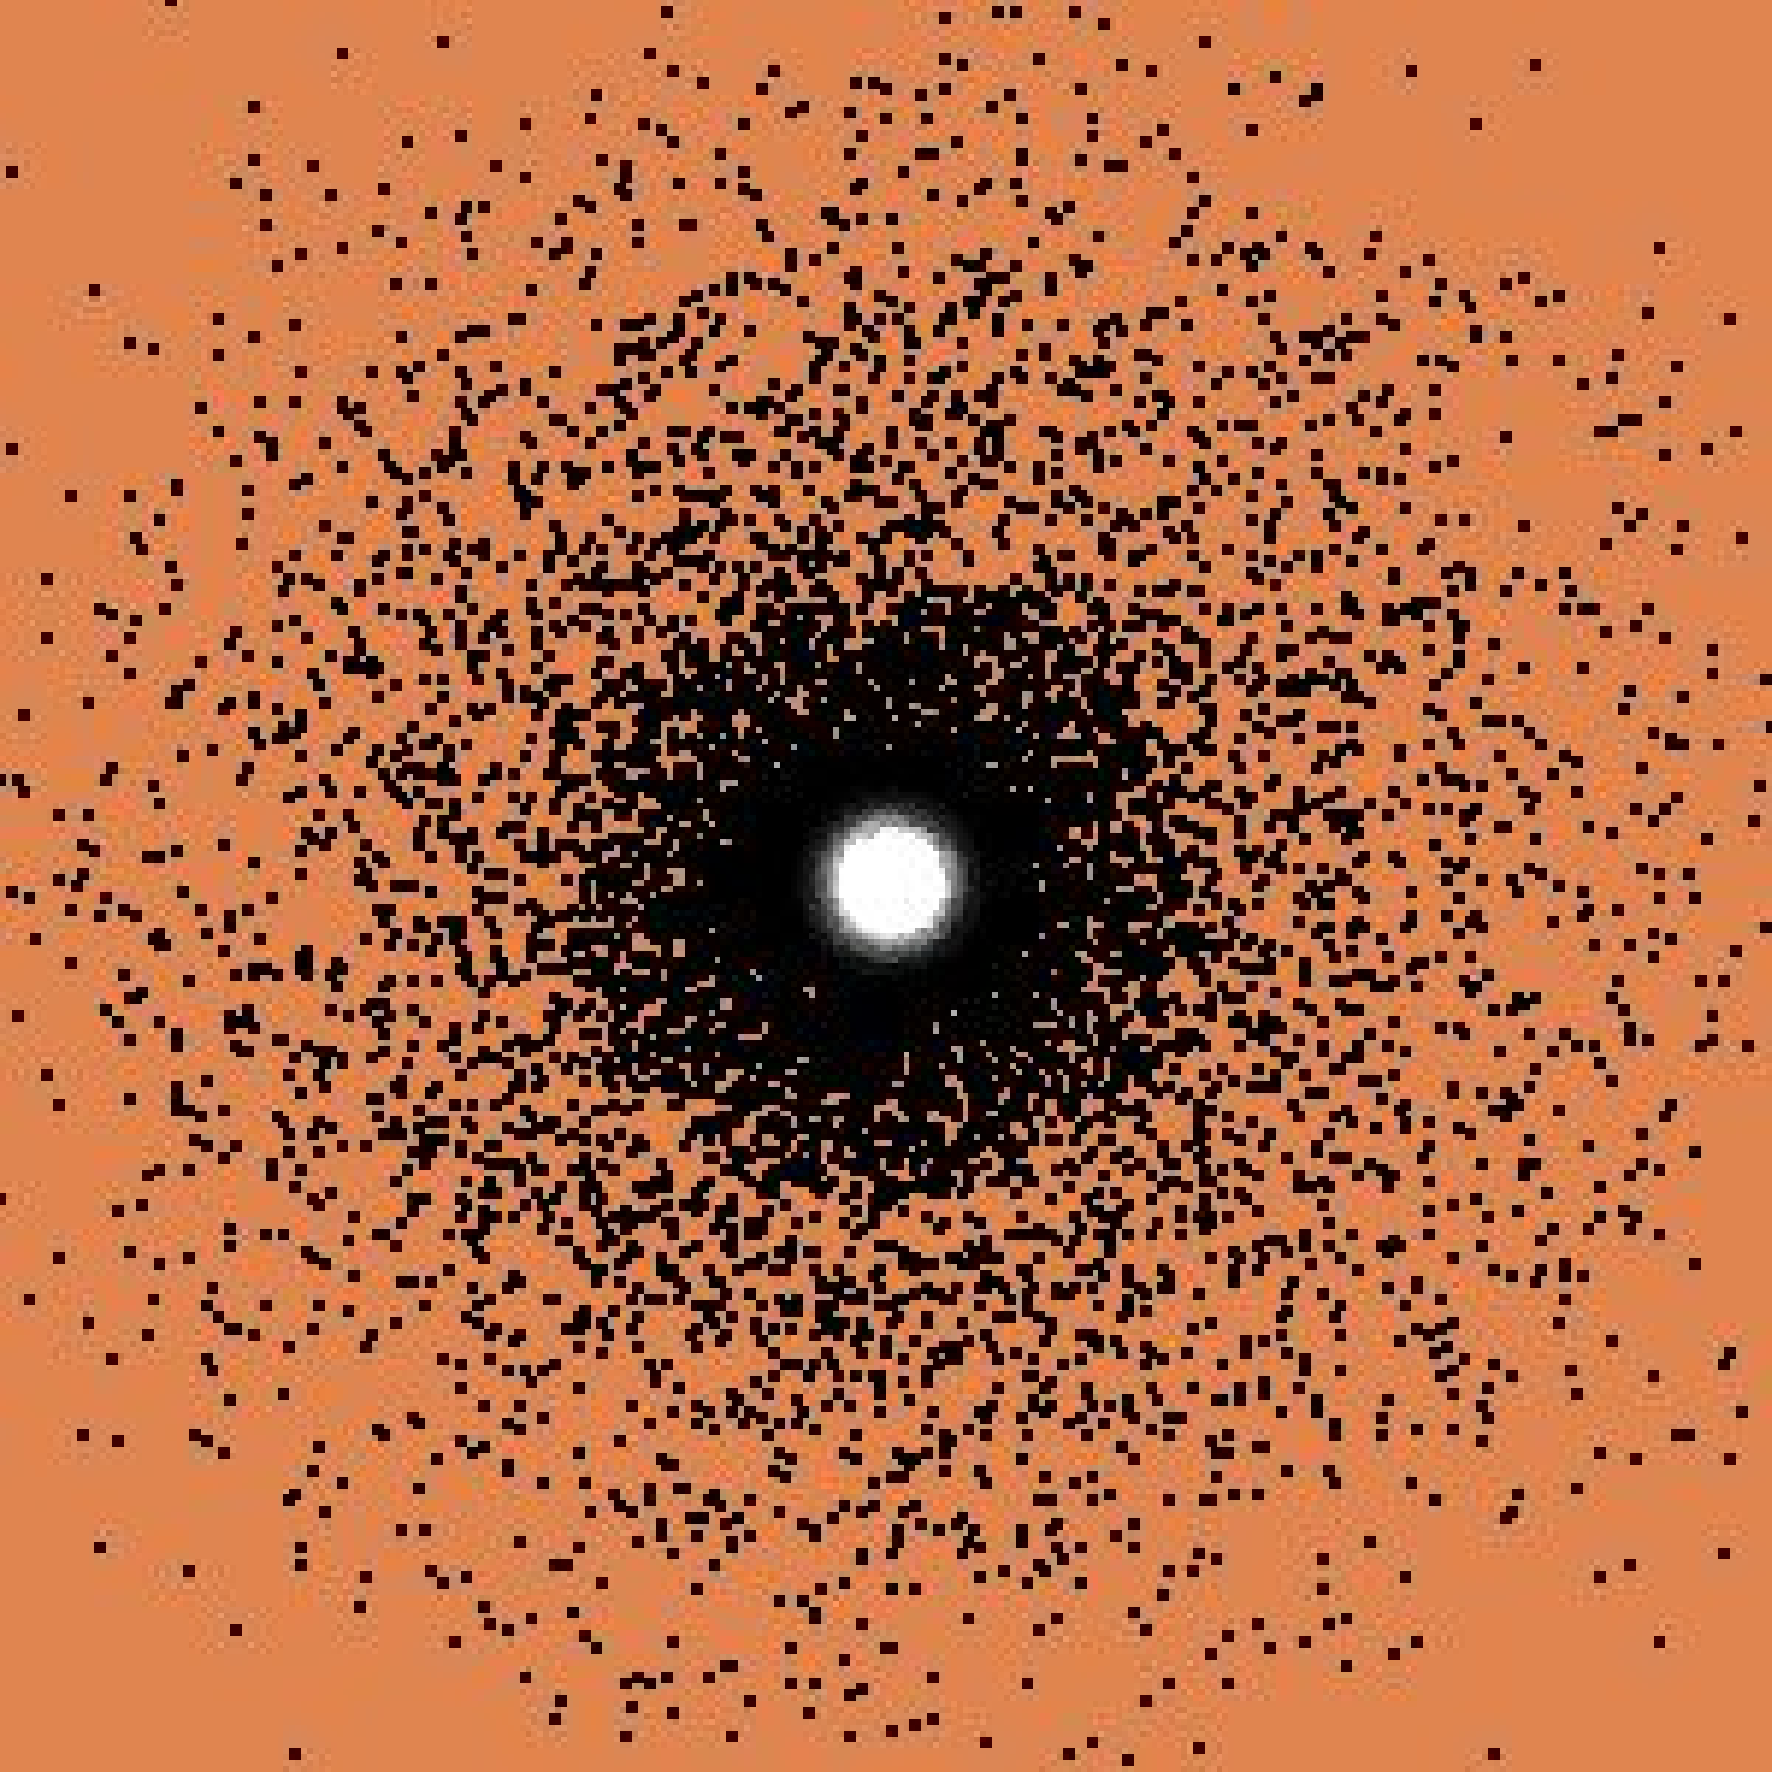
\includegraphics[width=\textwidth]{fixation3}
        \caption{}
    \end{subfigure}
    \hfill
    \centering
    \begin{subfigure}{0.20\textwidth}
        \centering
        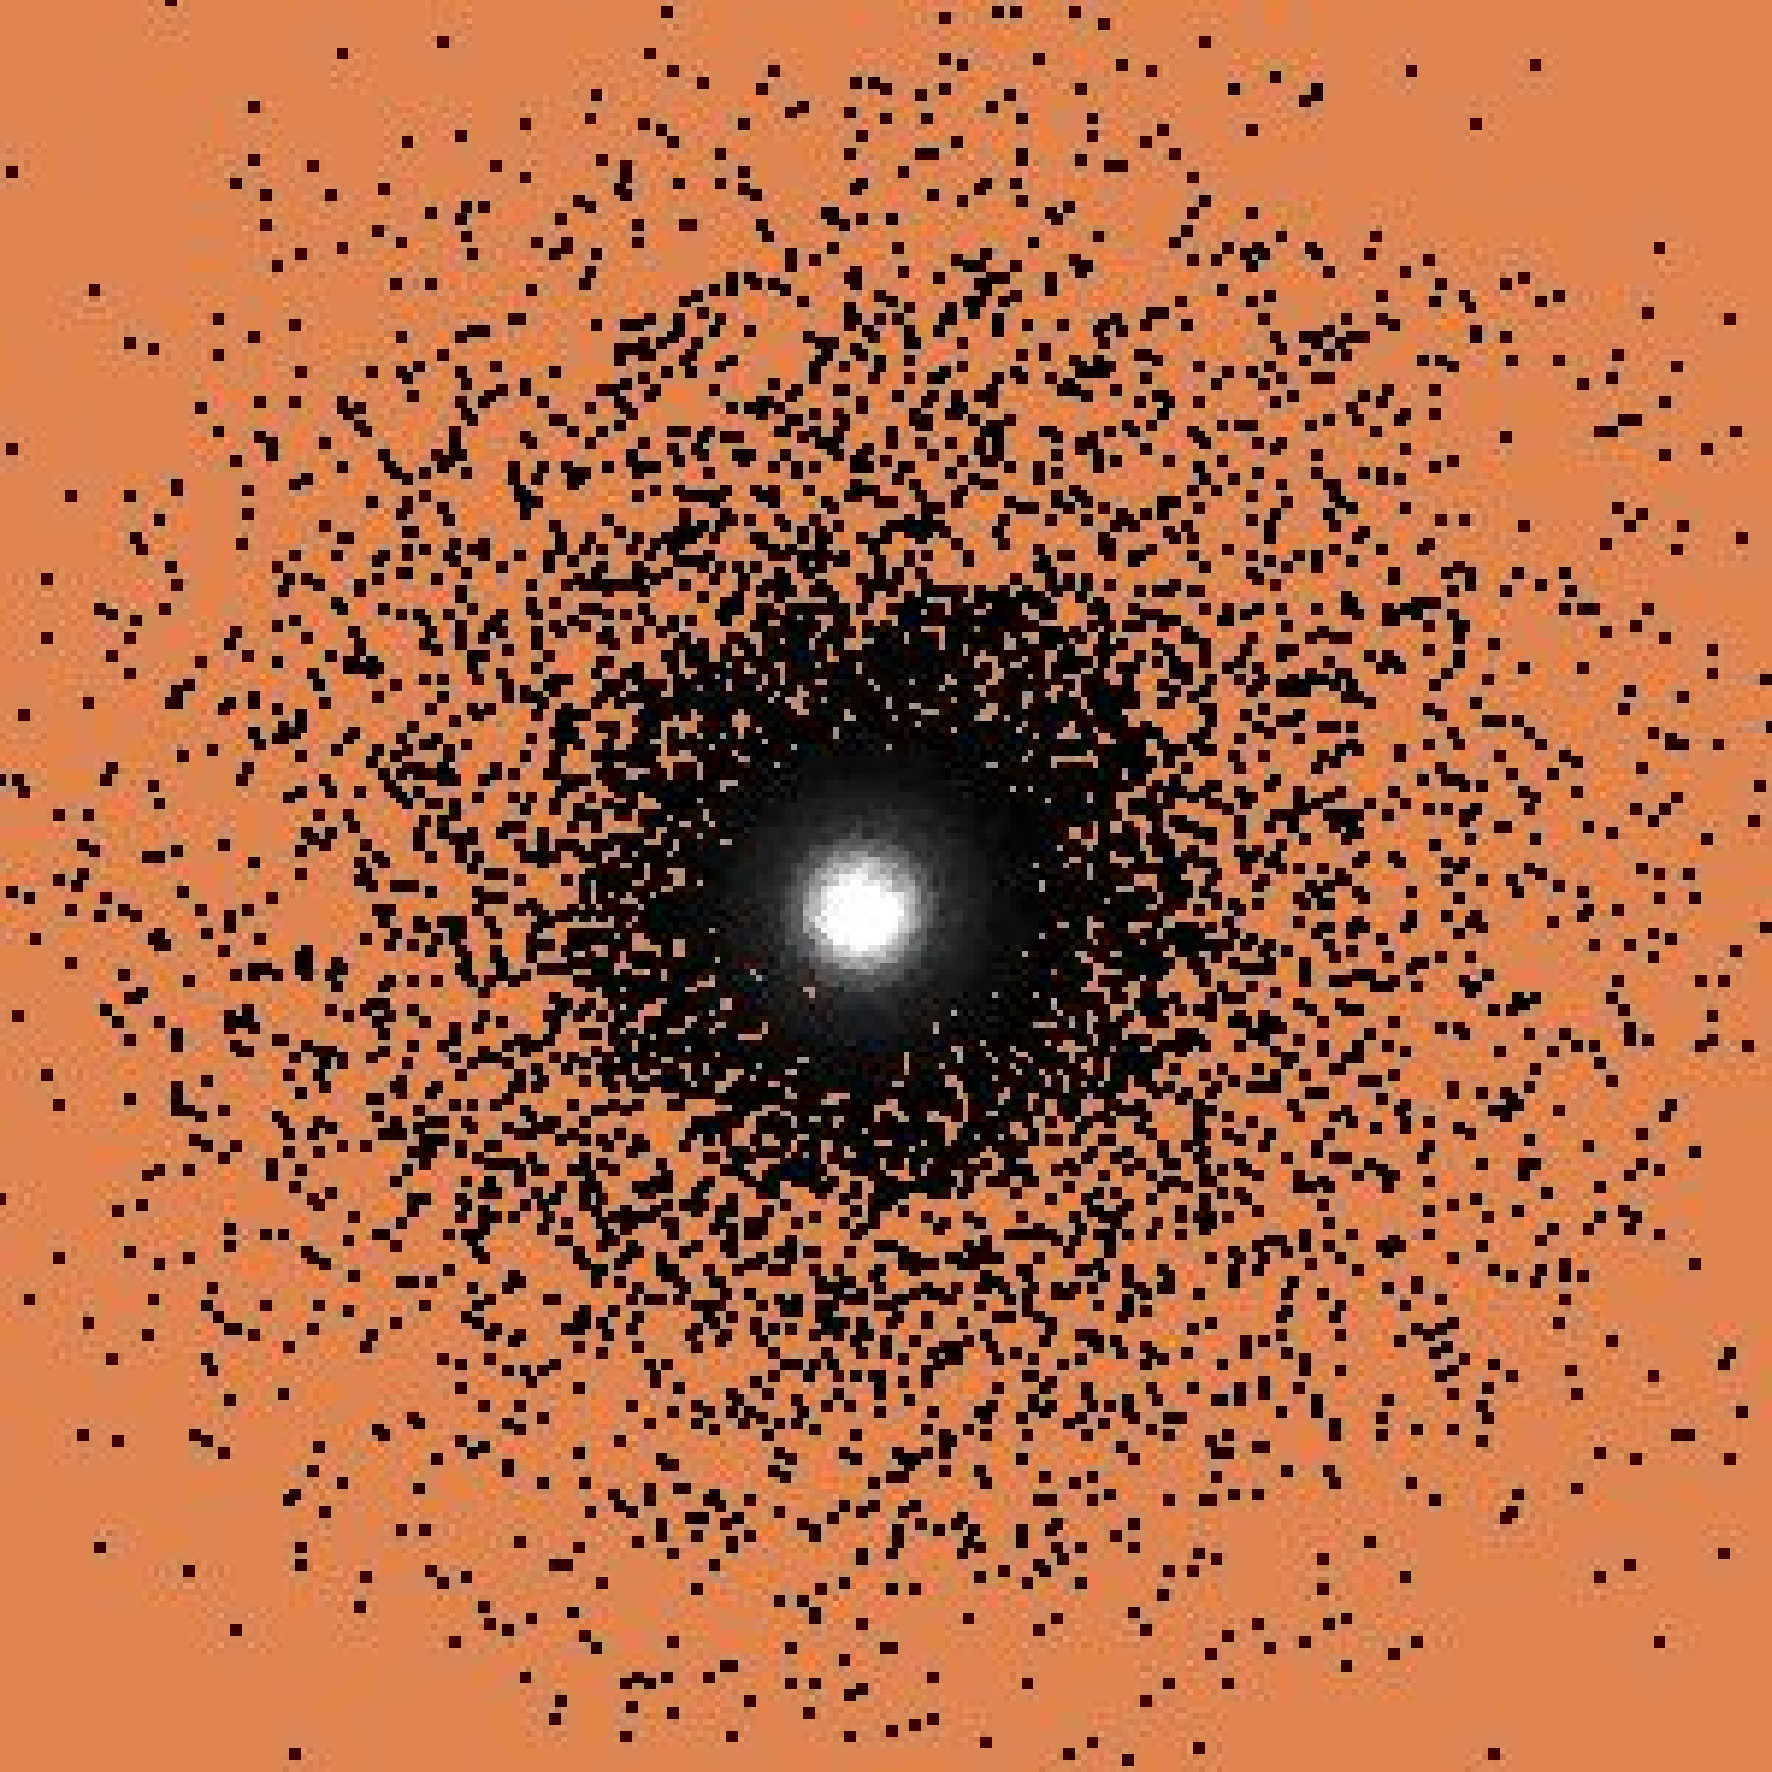
\includegraphics[width=\textwidth]{fixation4}
        \caption{}
    \end{subfigure}
    \hfill
    \centering
    \begin{subfigure}{0.20\textwidth}
        \centering
        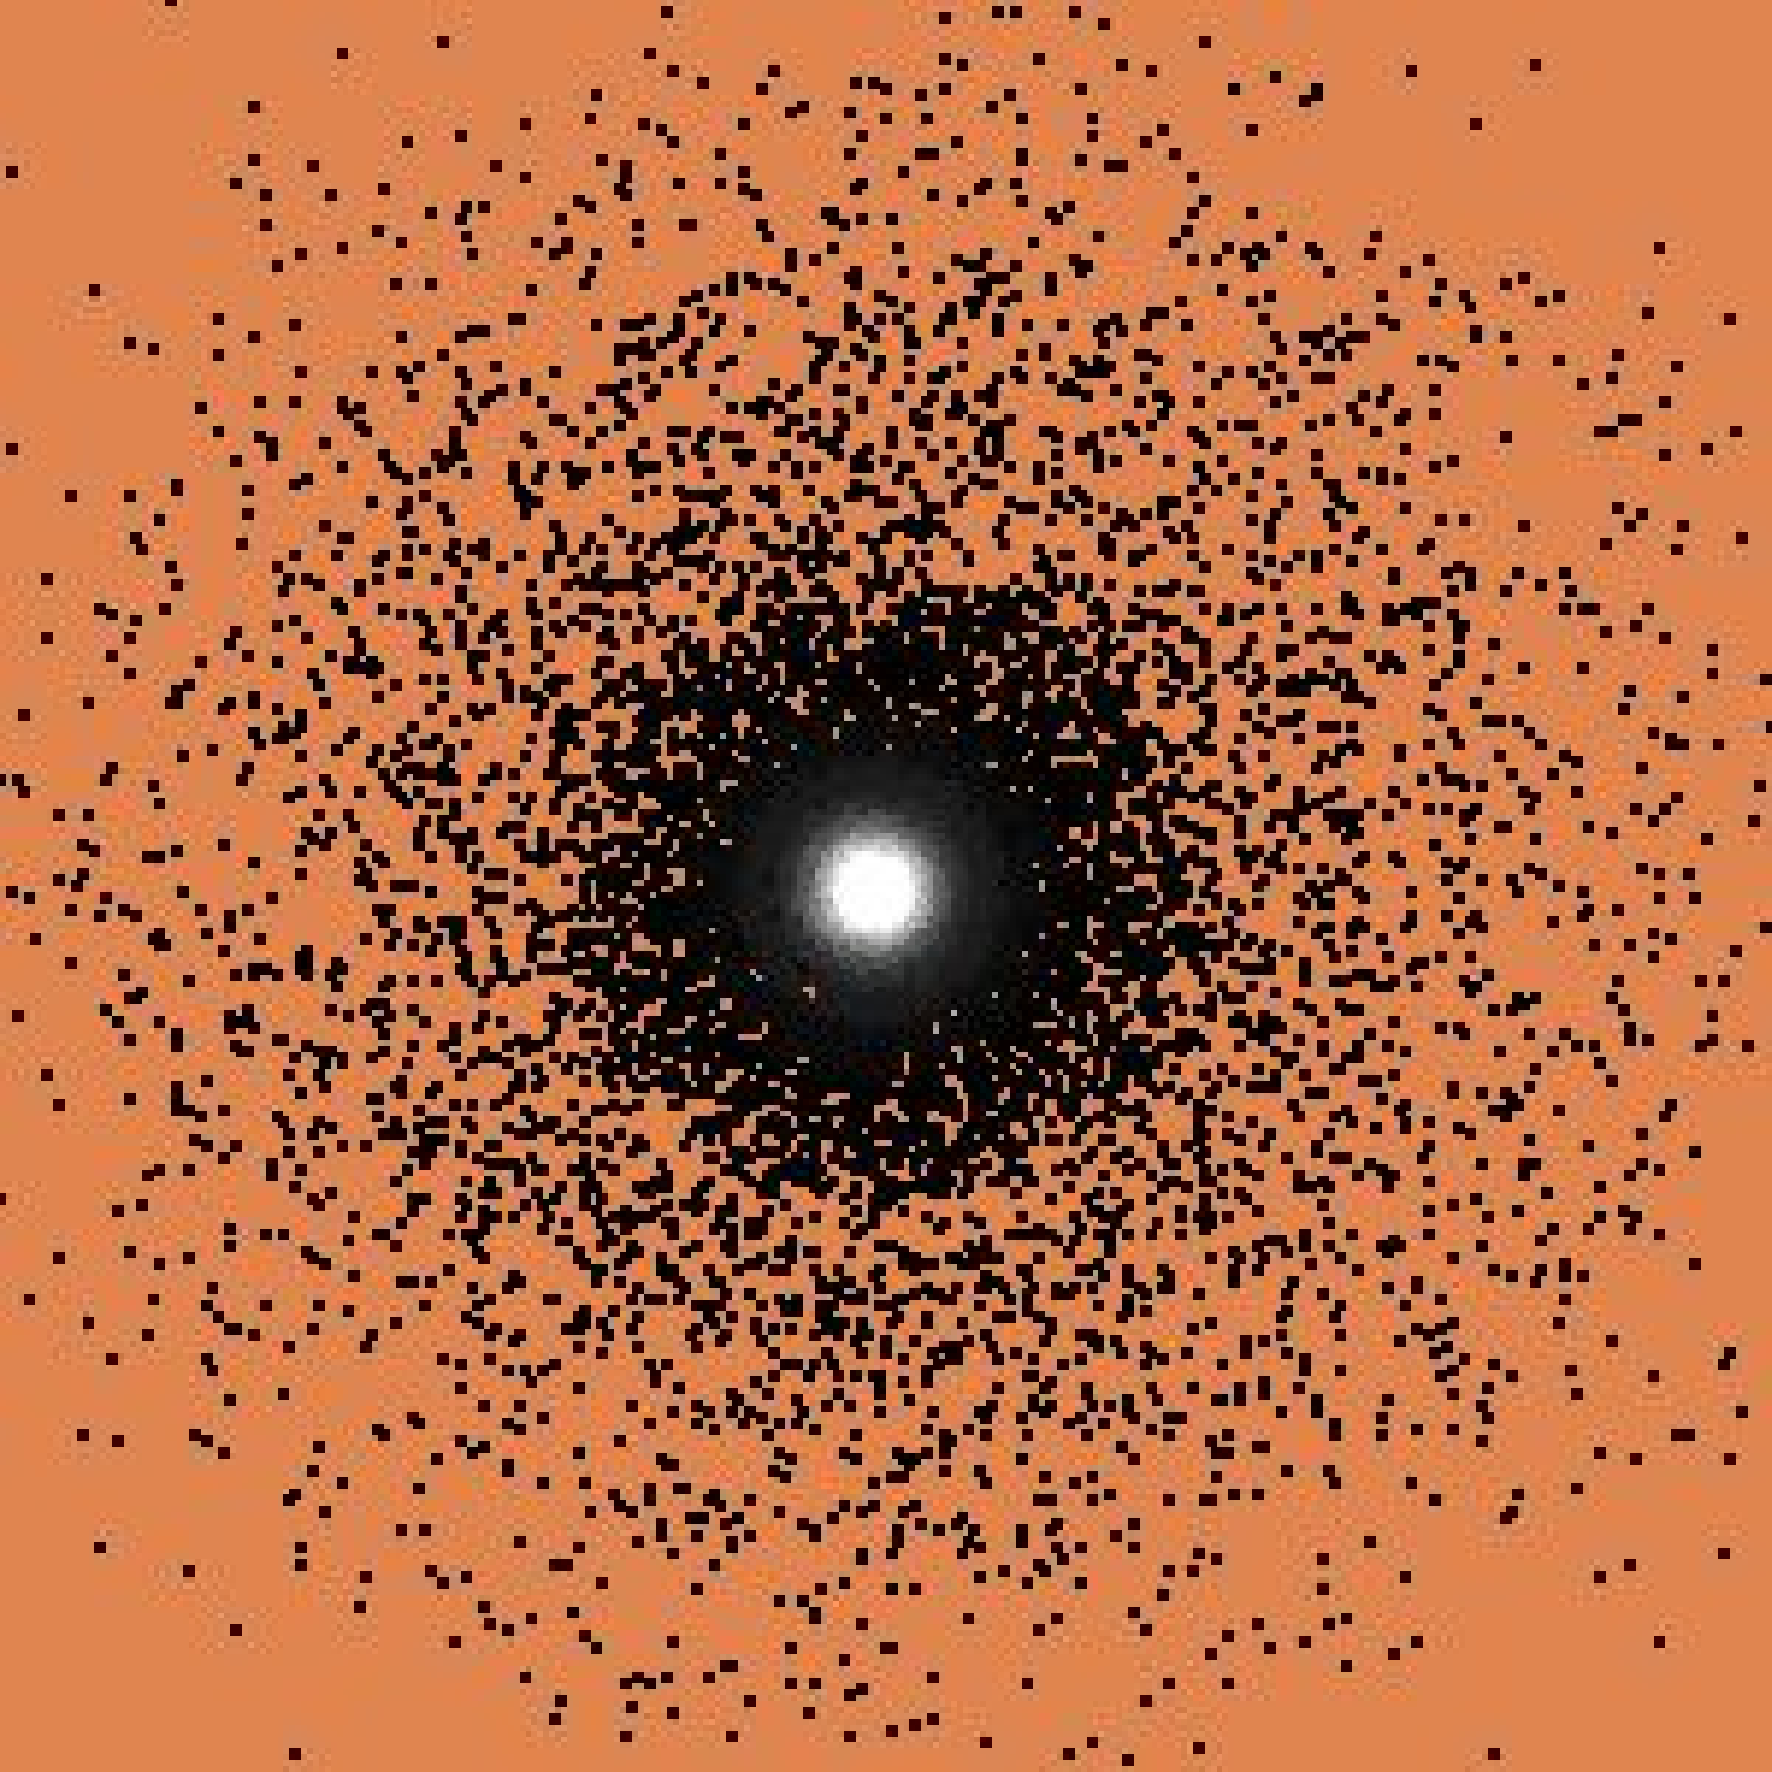
\includegraphics[width=\textwidth]{fixation5}
        \caption{}
    \end{subfigure}
    \caption[Fixation simulation with a SLiNet]{In (a), the ball has just entered the eye's field of view. In (b) the eye has fixated on the ball. In (c)-(d) we see micro-saccades in opposite directions, with a slight movement in (c) and a correction to reach the position in (d).}
    \label{fig:fixation}
\end{figure}

%********************************************************************%

\subsection{Smooth Pursuit}

The smooth pursuit test moves the target slowly in both the horizontal $\theta$ and vertical $\phi$ directions. We observe if our SLiNet can successfully track this motion in both directions at the same time; the results are summarized in Figure~\ref{fig:smooth}.

In Figure~\ref{fig:smooth_normal}, we compare the performance of the models when using the ONV. The LiNet performs much better here, tracking the ball almost perfectly. The eye still successfully tracks the target with the SLiNet, but it fixates on a position a few degrees off from the center of the ball. In Figure~\ref{fig:smooth_delta}, we plot the eye gaze that results from using the D-ONV. Here, the LiNet struggles to keep the target in the center of its field of view while the SLiNet follows its motion almost perfectly. However, the motion that results from using the SLiNet is also more noisy. This is a result of micro-saccadic motion, where the eye moves slightly in one direction and then moves in the opposite direction in the next movement to compensate.
% Finally, in Figure~\ref{fig:smooth_hybrid} we see that using our Hybrid SLiNet with just ReLU activated layer results in smooth performance.

\begin{figure}
    \centering
    \begin{subfigure}{\textwidth}
        \centering
        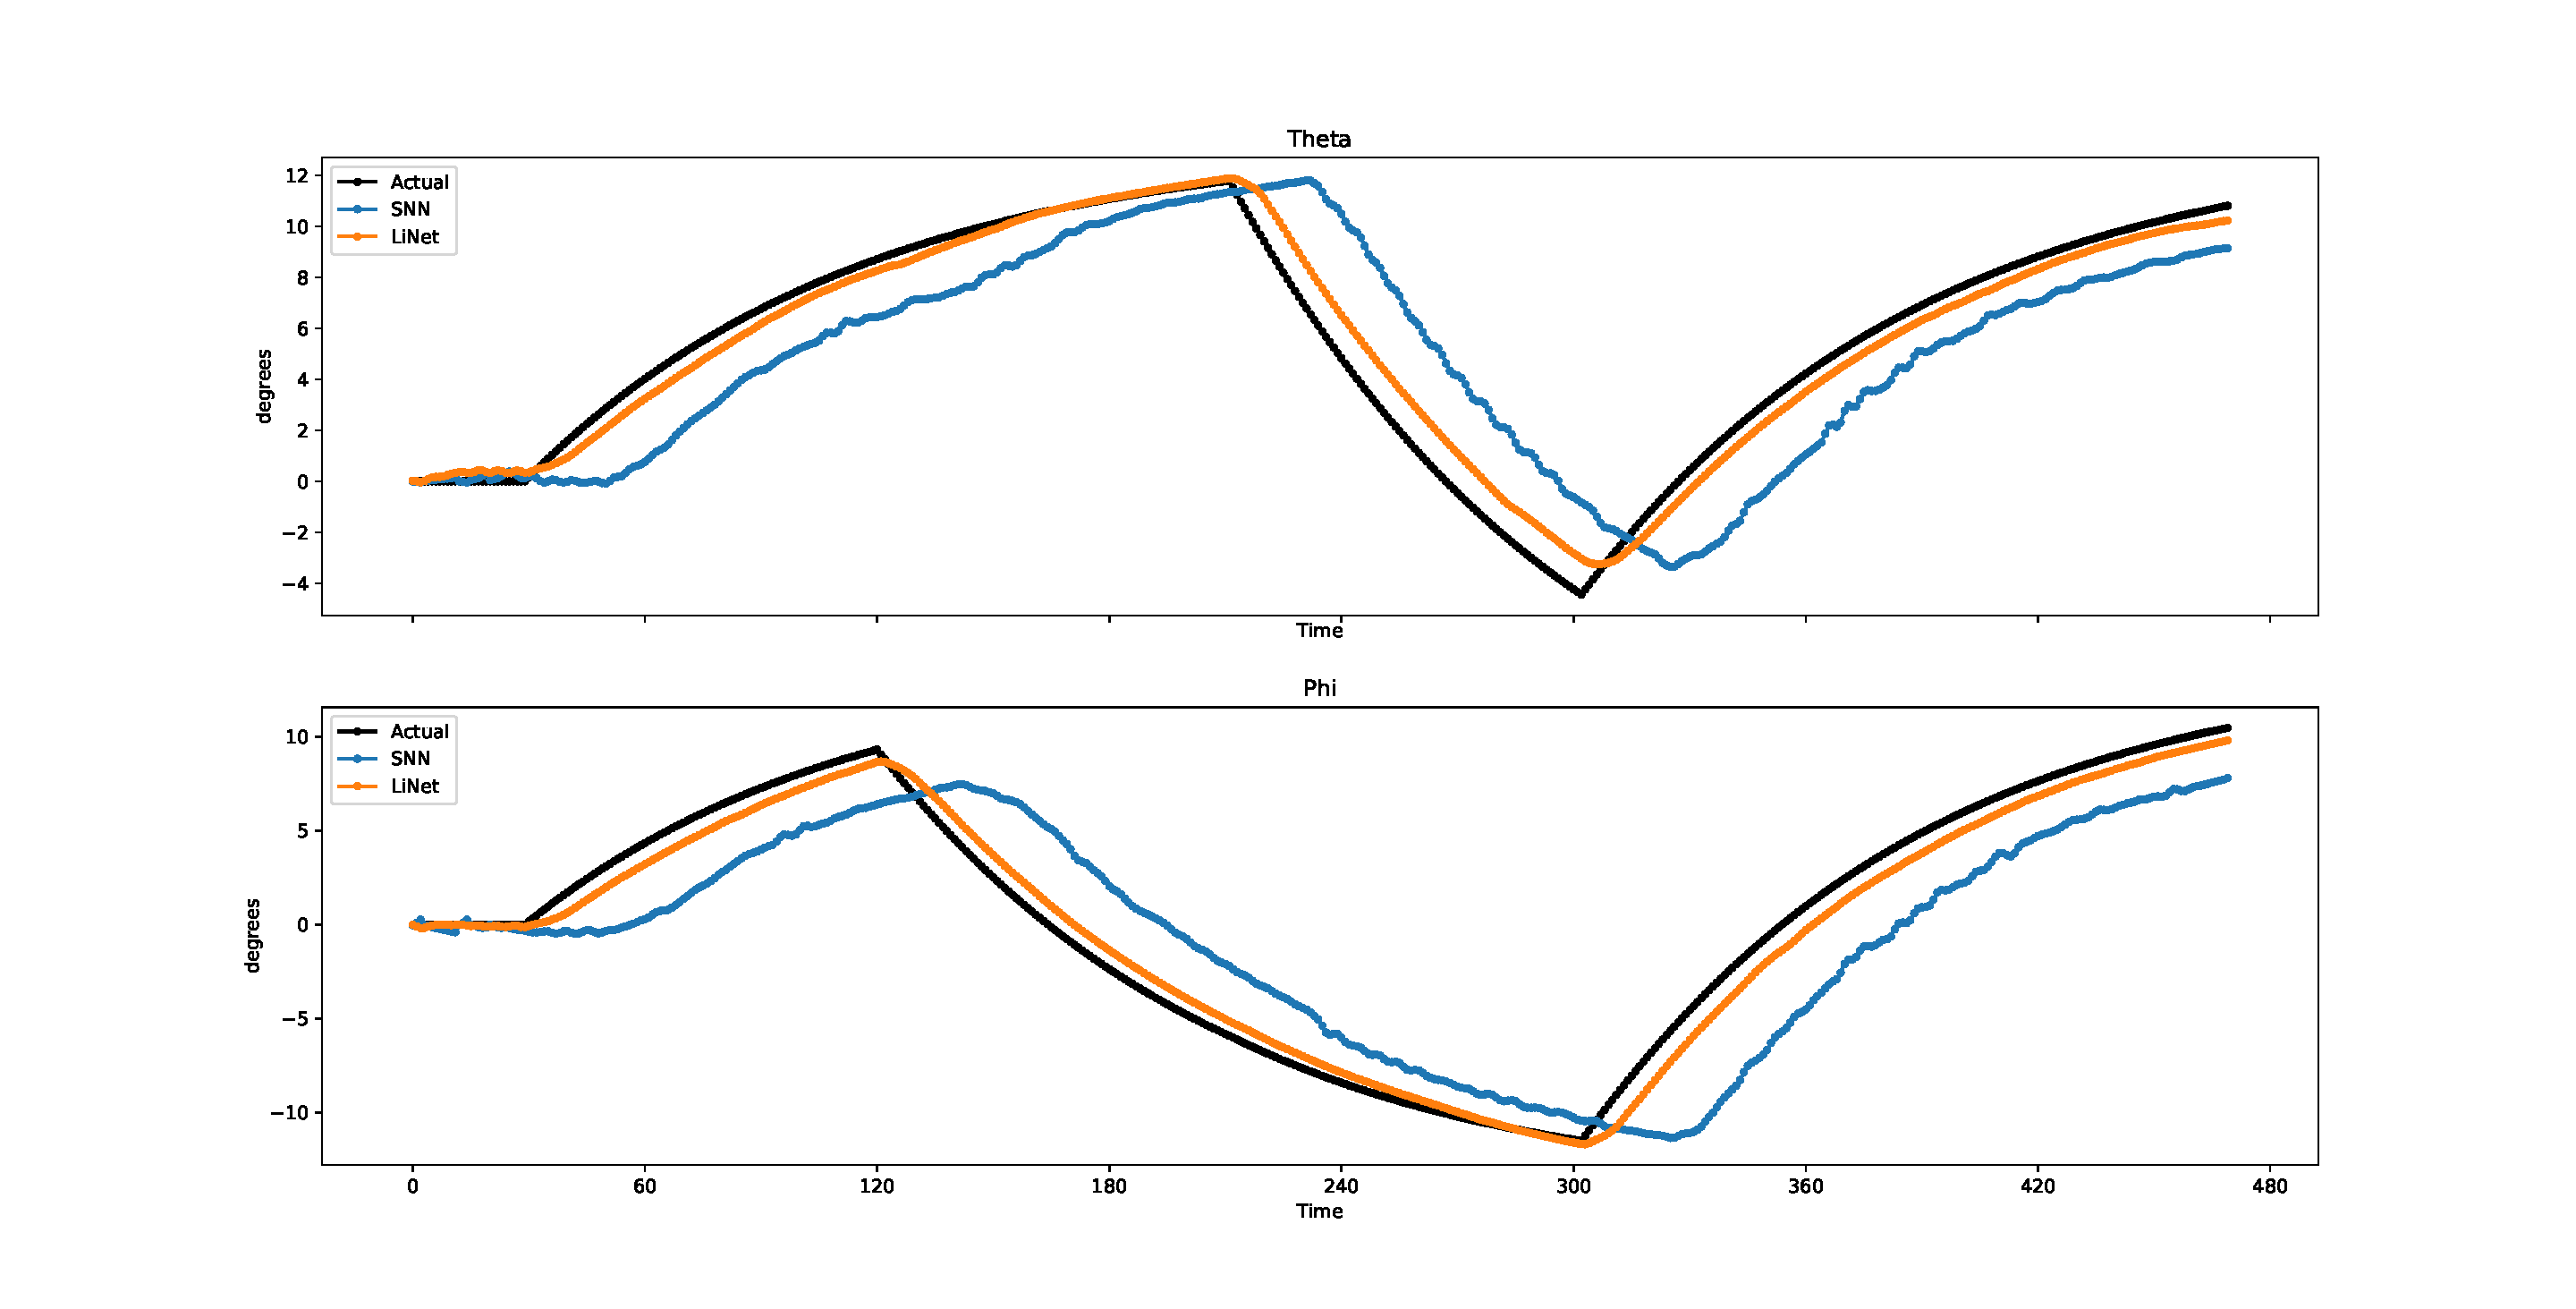
\includegraphics[width=\textwidth]{smooth_normal}
        \caption{}
        \label{fig:smooth_normal}
    \end{subfigure}
    \begin{subfigure}{\textwidth}
        \centering
        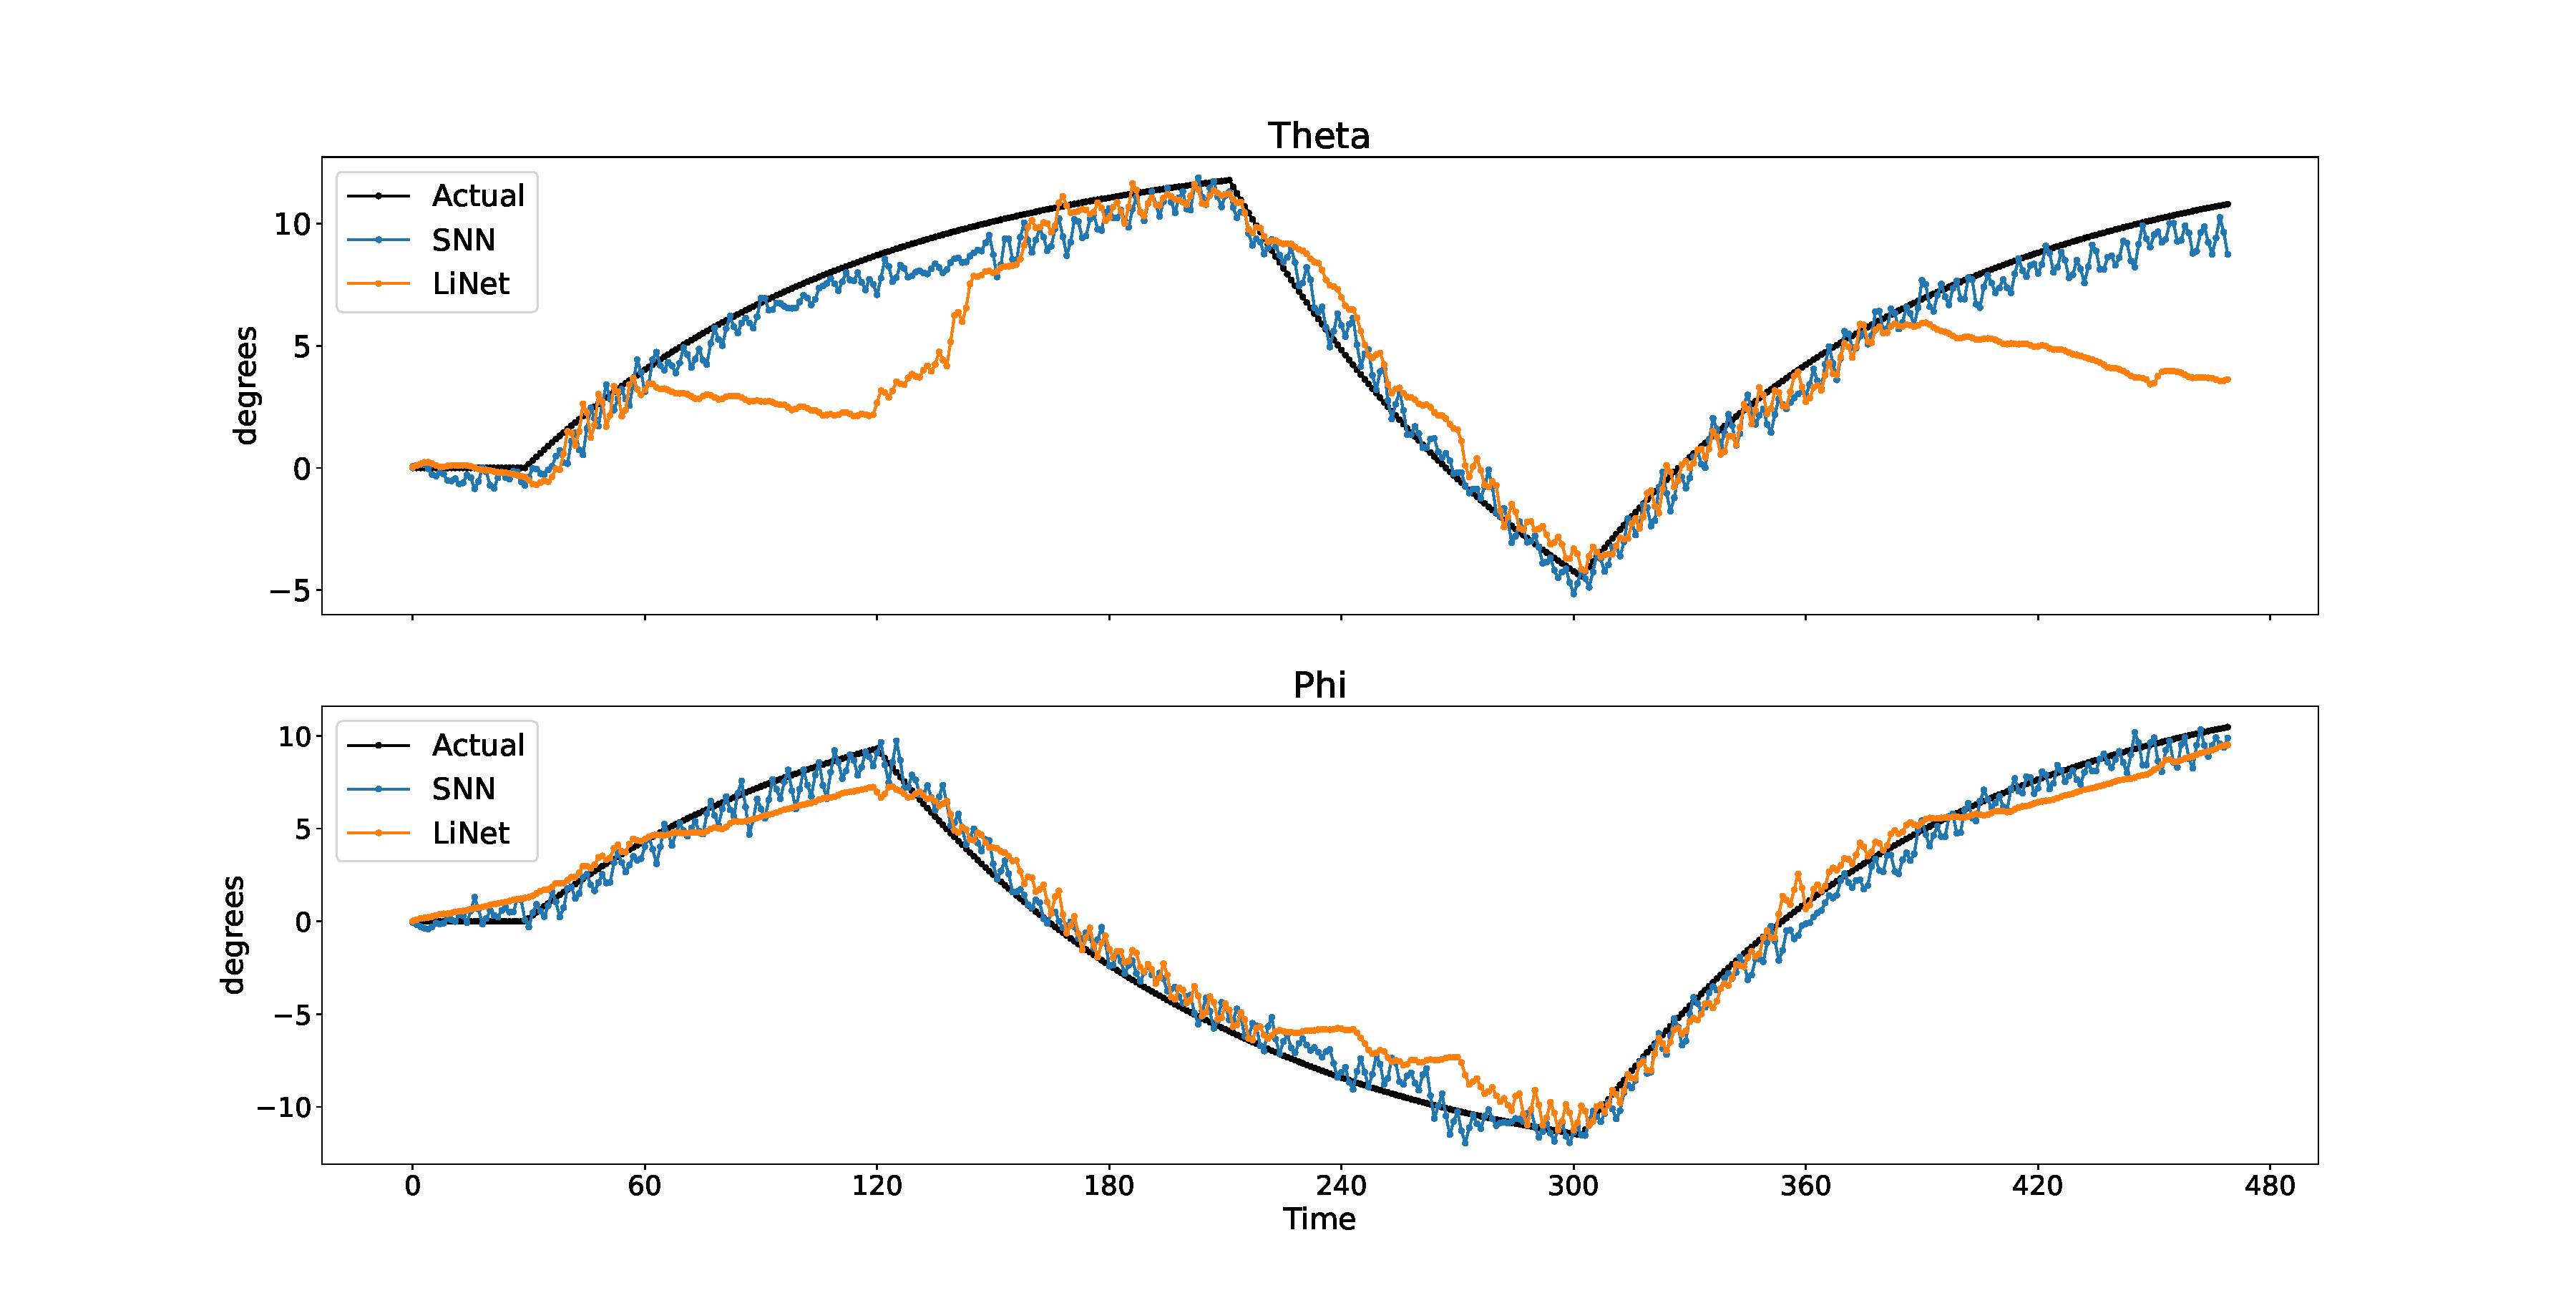
\includegraphics[width=\textwidth]{smooth_delta}
        \caption{}
        \label{fig:smooth_delta}
    \end{subfigure}
    \caption[Smooth pursuit eye displacement with different models]{We compare the smooth movement of the target with the eye's gaze direction using different foveation networks. (a) The LiNet performs better using the ONV, but the SLiNet also keeps the target roughly in the center. (b) The SLiNet is far better at tracking the target when using a D-ONV.}
    \label{fig:smooth}
\end{figure}

Our SLiNet, albeit noisy, tracks the target successfully using either the ONV or D-ONV.

%********************************************************************%

\subsection{Saccade}

In a real saccade, the eye moves rapidly to fixate on a new location. To re-create this movement, we allow the eye to fixate on the ball and then rapidly move it to a new point within the eye's field of view. The results are summarized in Figure~\ref{fig:saccade}. Note that the seemingly instantaneous jumps in the black line represent saccadic movement where the ball rapidly moves to a new location in the eye's field of view.

In Figure~\ref{fig:saccade_normal}, we input an ONV to our two models. They exhibit similar performances, successfully tracking the target and keeping it focused on the center of the retina. When using the D-ONV, shown in Figure~\ref{fig:saccade_delta}, we see a difference between the two models. The SLiNet tracks the target better, exhibiting the same noisy motions as in the smooth motion test; however, the LiNet causes the eye to drift away from the target after about 4 consecutive saccadic motions. 
% Finally, in Figure~\ref{fig:saccade_hybrid} we again note that our Hybrid SLiNet creates smooth tracking motions while using the D-ONV.

\begin{figure}
    \centering

    \begin{subfigure}{\textwidth}
        \centering
        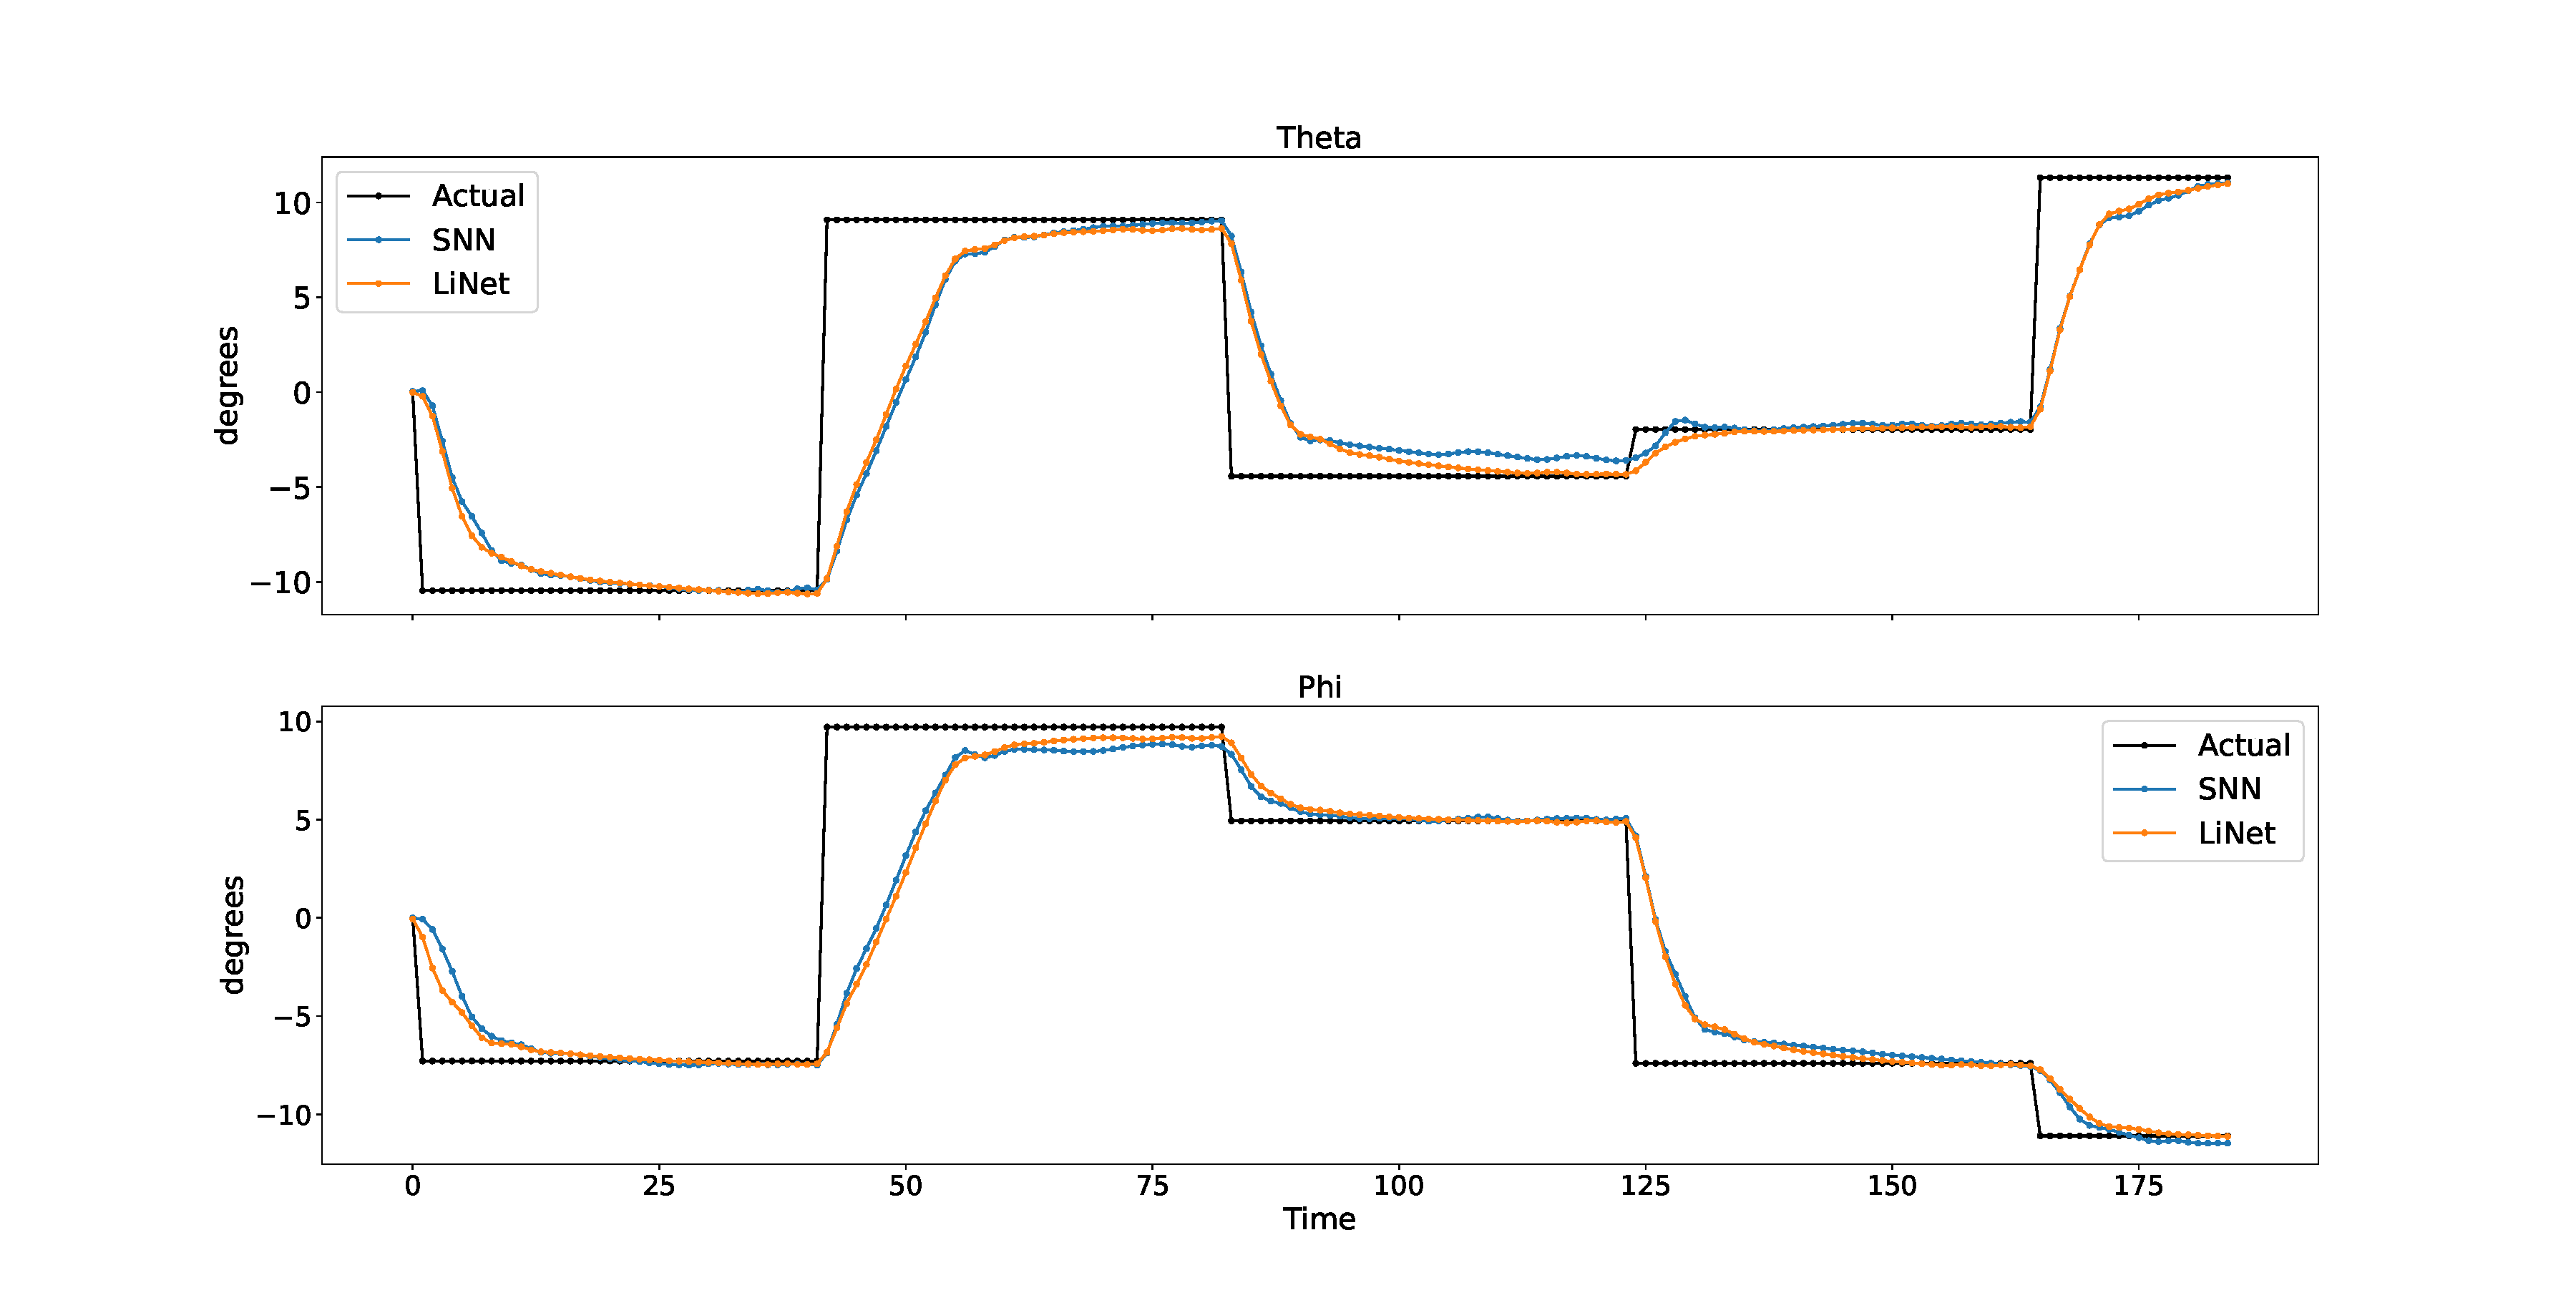
\includegraphics[width=\textwidth]{saccade_ori_normal}
        \caption{}
        \label{fig:saccade_normal}
    \end{subfigure}

    \begin{subfigure}{\textwidth}
        \centering
        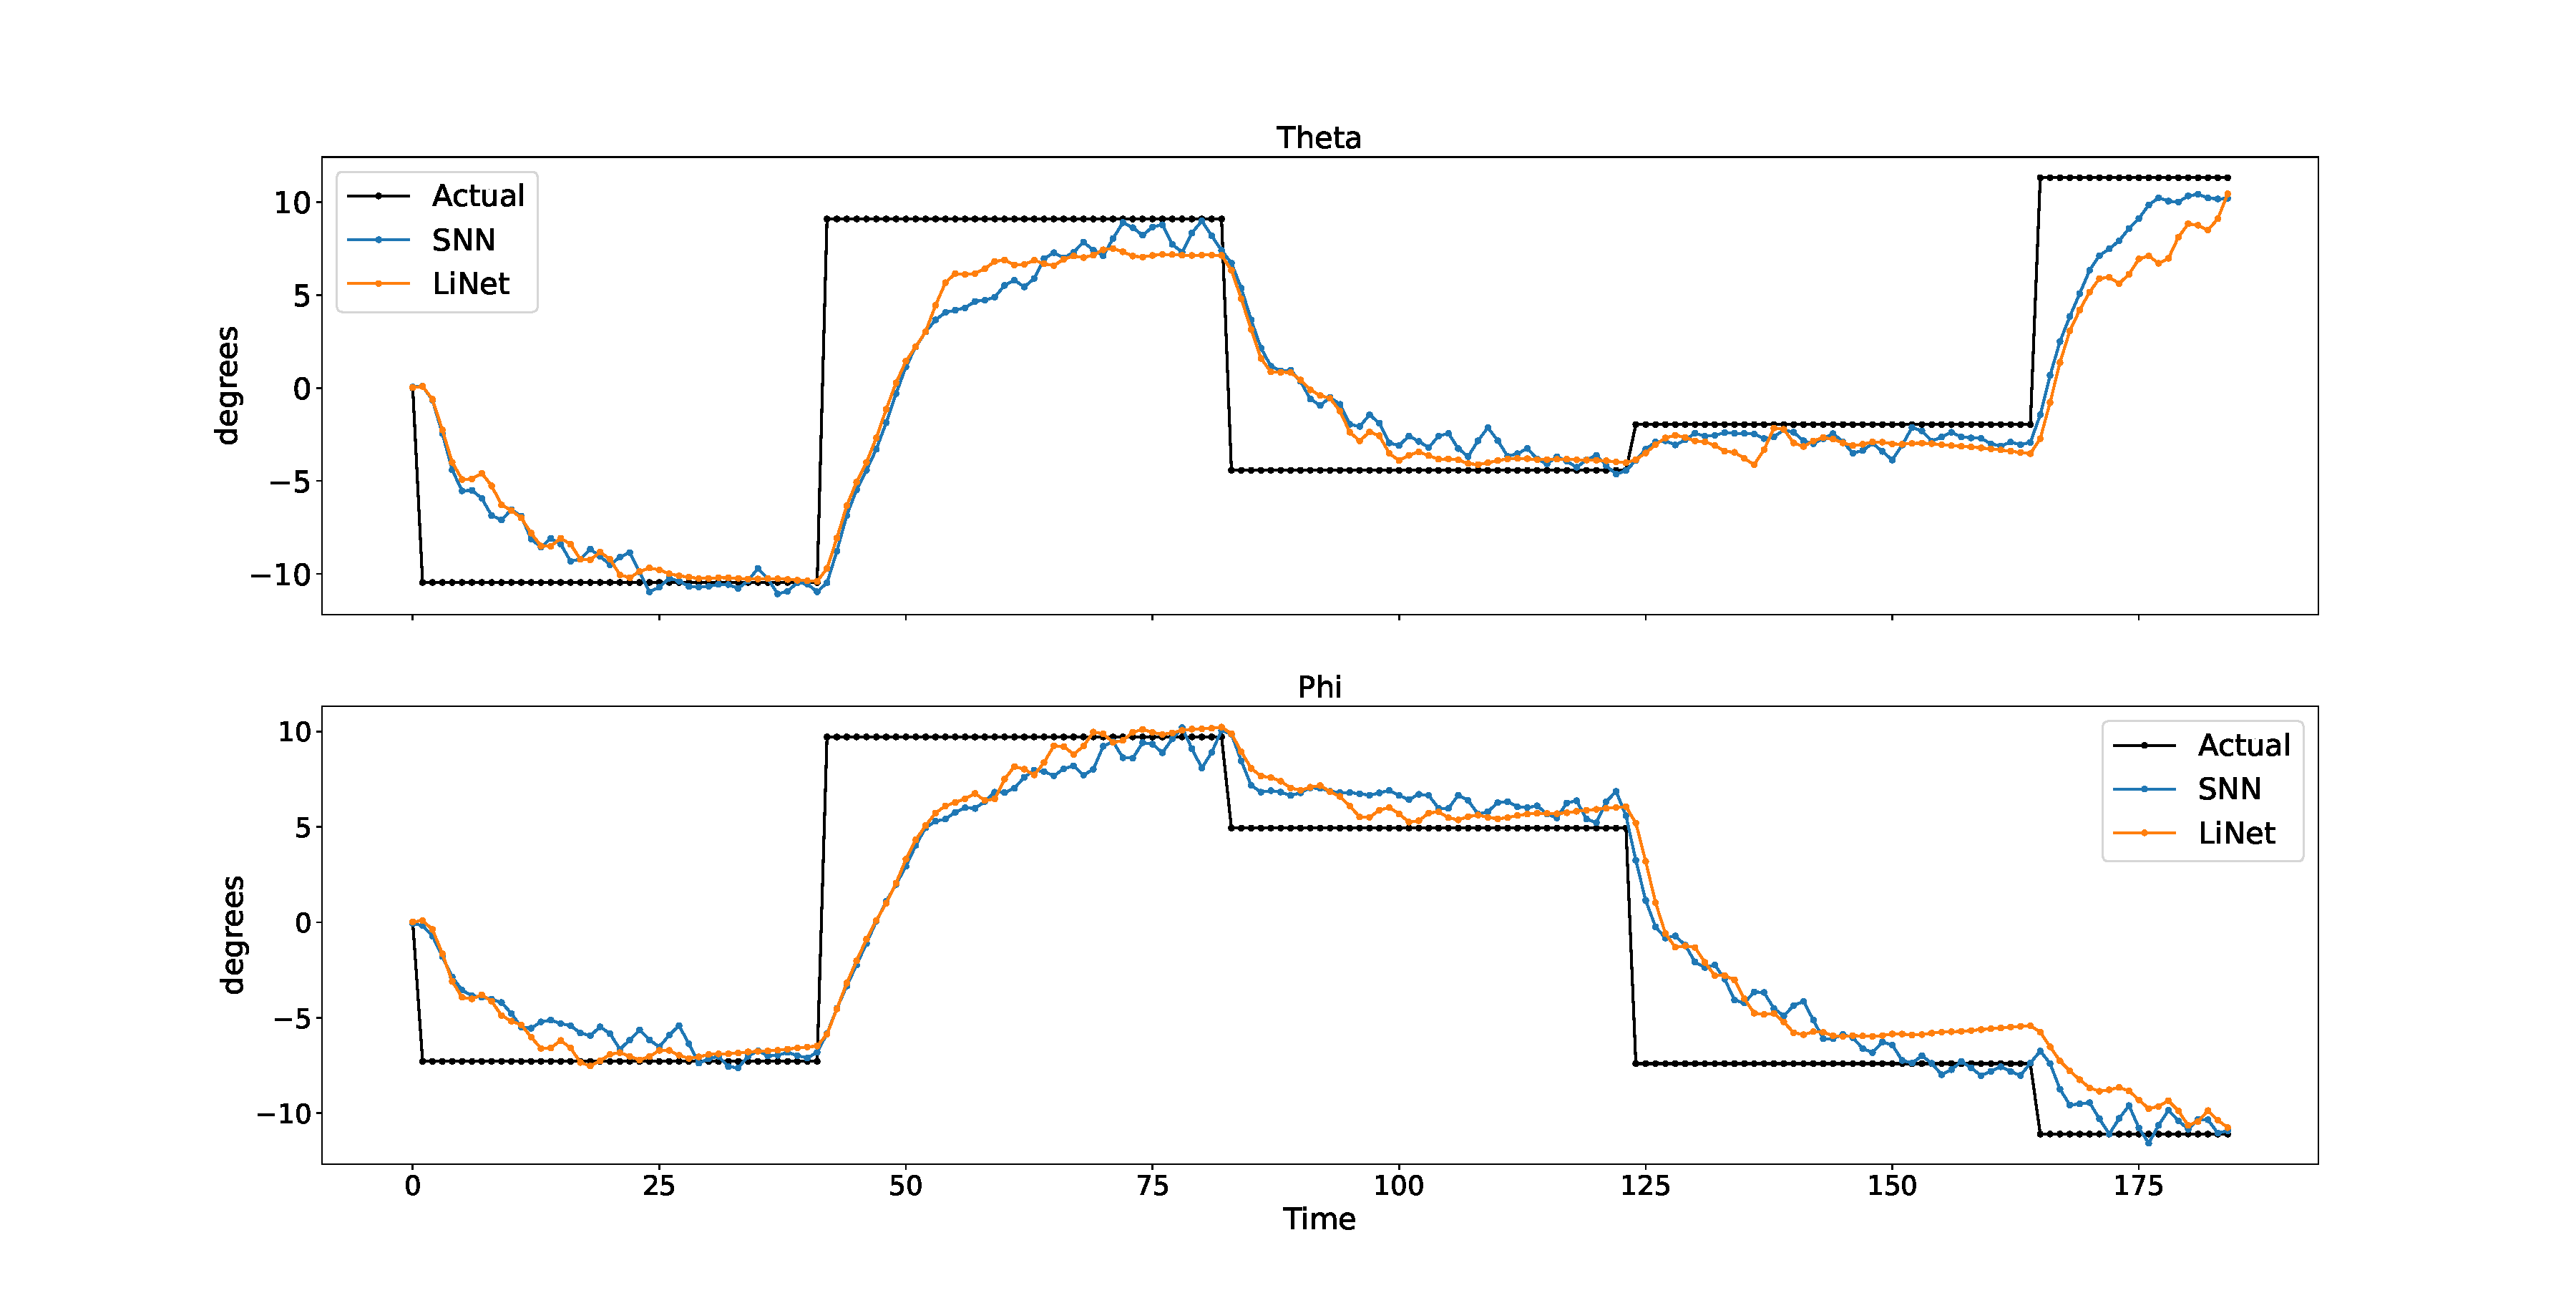
\includegraphics[width=\textwidth]{saccade_ori_delta}
        \caption{}
        \label{fig:saccade_delta}
    \end{subfigure}

    \caption[Saccade eye orientation with different models]{We compare the saccadic movement of the target with the center of the eye's gaze using the SLiNet and LiNet foveation networks. (a) Both models have similar performance, and are able to track the ball accurately. (b) The LiNet drifts away from the target after the fourth saccadic movement, whereas the SLiNet successfully tracks the target with a slightly noisy movement.}
    \label{fig:saccade}
\end{figure}

Our SLiNet, albeit noisy, tracks the target successfully. It also keeps the target in the center of the fovea when using the D-ONV, unlike the LiNet.

%********************************************************************%
\section{Comparison with Human Eye Movement}
%********************************************************************%

In this section we compare the angular displacement, velocity, and acceleration of our eye model to those of real human subjects. We use two movement patterns for the target to do so. The human recordings for smooth movement come from the work of \citet{human_smooth_lateral}, while the recordings for saccadic movement come from \citet{human_eye}.

\subsection{Smooth Lateral Movement}

We compare the angular displacements that result from moving our target back and forth in the horizontal direction. As seen in Figure~\ref{fig:smooth_lateral}, this results in a sinusoidal curve. Both models successfully track the ball when using the ONV, as seen in Figure~\ref{fig:smooth_lateral_normal}. The motions are relatively smooth, whereas the curve from the human subject in Figure~\ref{fig:smooth_lateral_human} includes noisy movement. Our SLiNet produces these noisy movements when using the D-ONV, shown in Figure~\ref{fig:smooth_lateral_delta}. The LiNet's motion is not realistic and causes the eye to drift away.

\begin{figure}
    \centering

    \begin{subfigure}{0.3\textwidth}
        \centering
        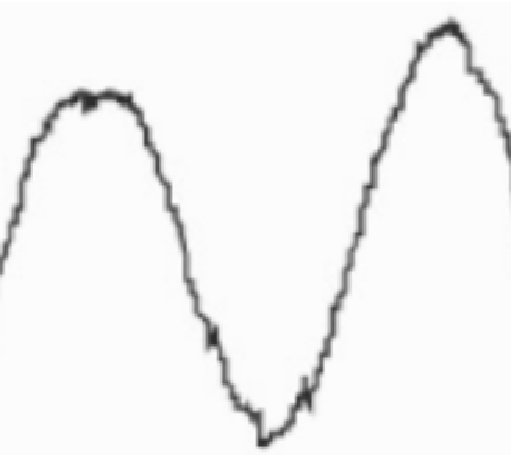
\includegraphics[width=\textwidth]{smooth_lateral_human}
        \caption{}
        \label{fig:smooth_lateral_human}
    \end{subfigure}
    \hfill
    \begin{subfigure}{0.3\textwidth}
        \centering
        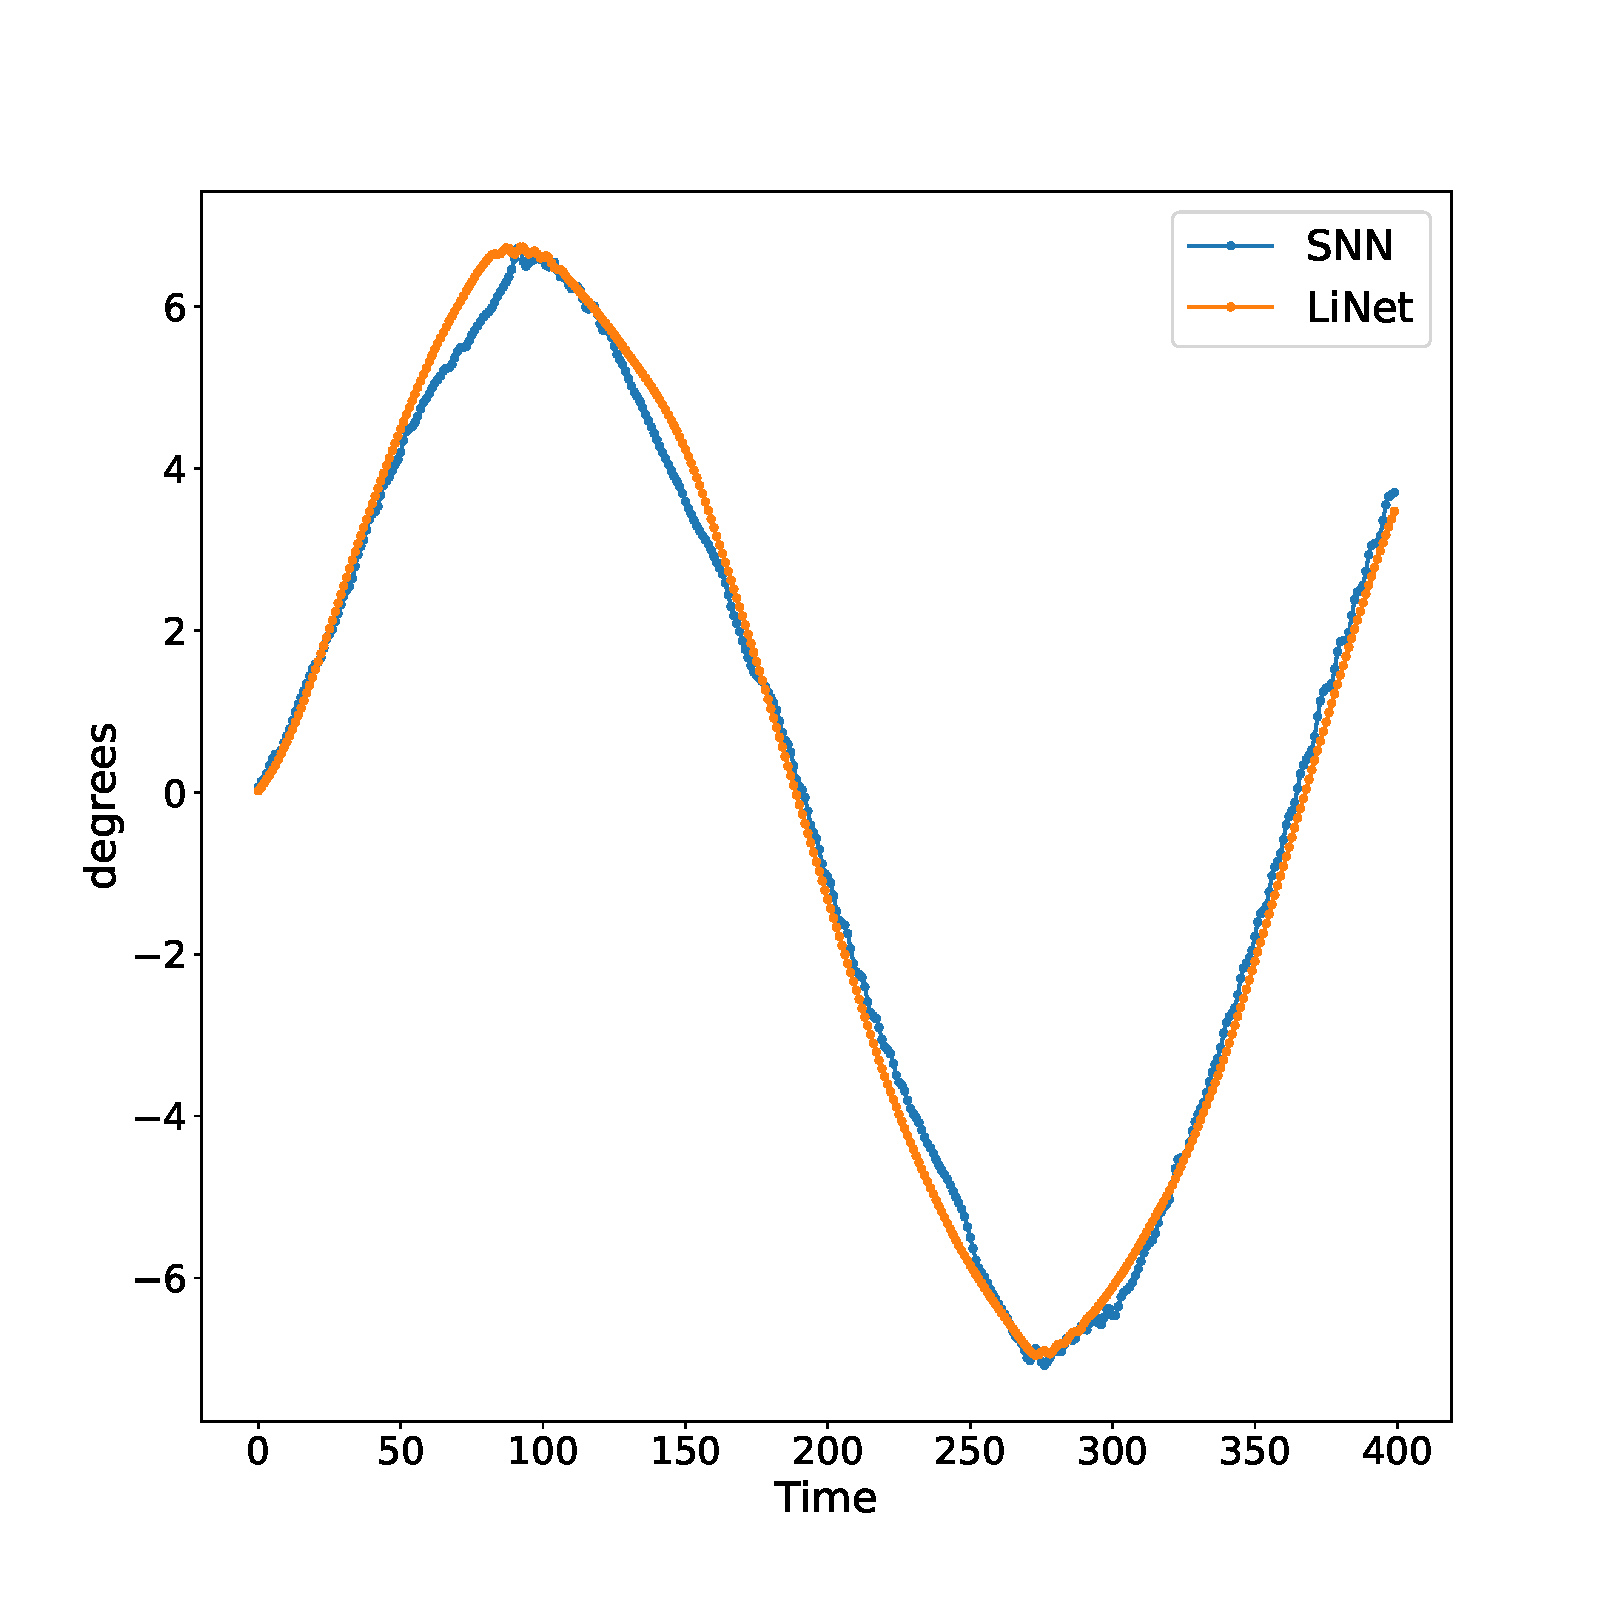
\includegraphics[width=\textwidth]{smooth_lateral_normal}
        \caption{}
        \label{fig:smooth_lateral_normal}
    \end{subfigure}
    \hfill
    \begin{subfigure}{0.3\textwidth}
        \centering
        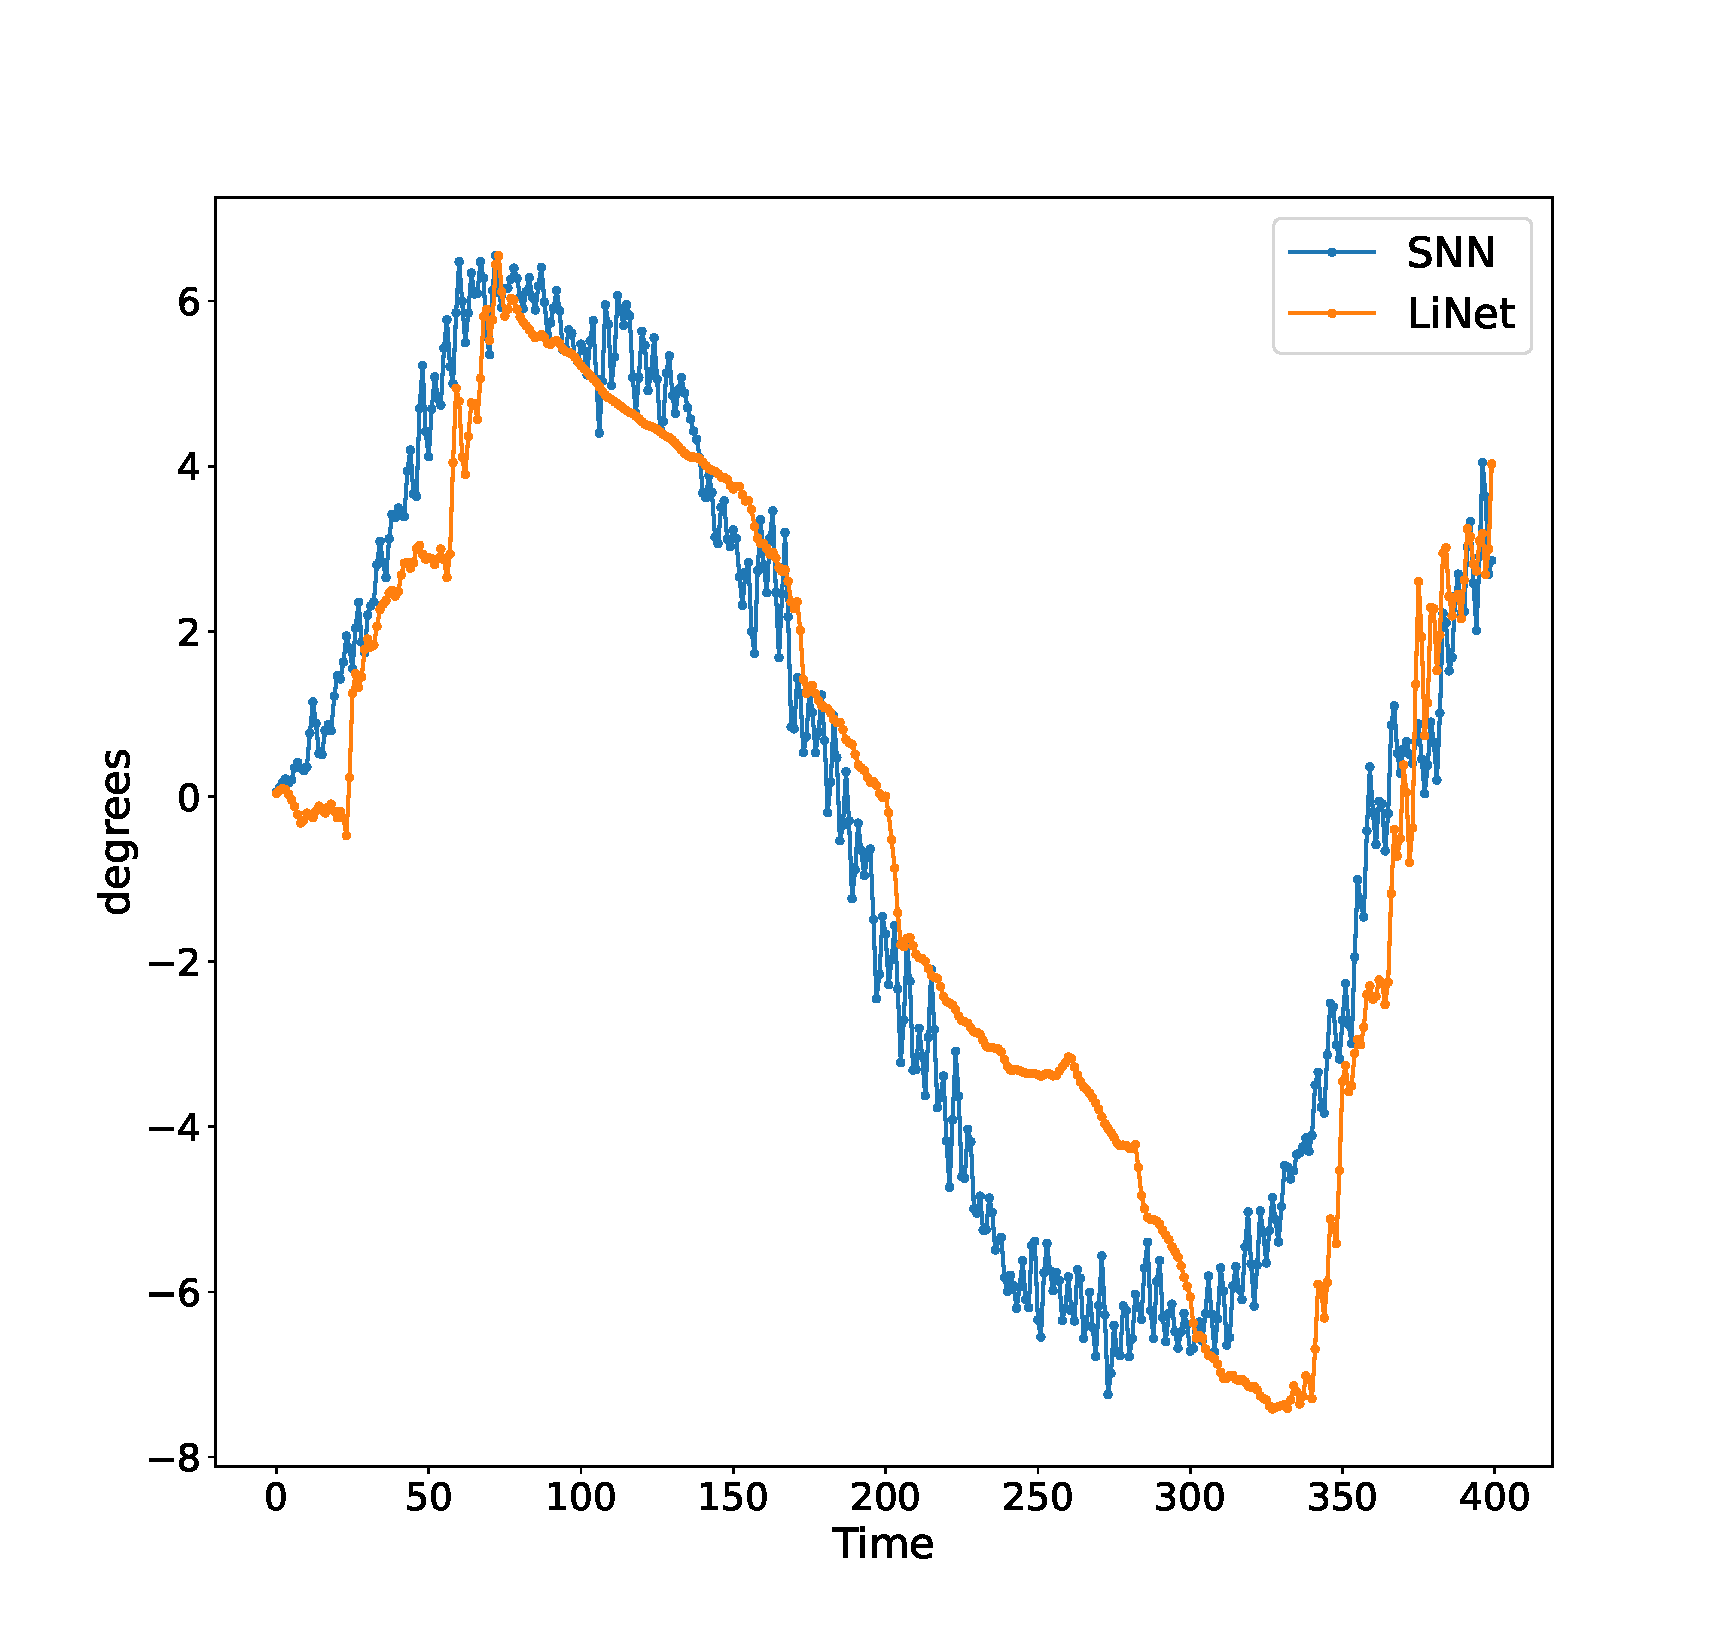
\includegraphics[width=\textwidth]{smooth_lateral_delta}
        \caption{}
        \label{fig:smooth_lateral_delta}
    \end{subfigure}
    \caption[Angular displacements from sinusoidal motion, compared to a human subject.]{Comparison of angular displacements on horizontal motion. (a) Human. (b) ONV input. (c) D-ONV input.}
    \label{fig:smooth_lateral}
\end{figure}

%********************************************************************%

\subsection{Saccade}

We again use saccadic motion, but this time note the angular velocity and acceleration of our eye model's movements in addition to the eye gaze direction. We compare these movements to those of a real human subject.

\begin{figure}
    \centering

    \begin{subfigure}{0.2\textwidth}
        \centering
        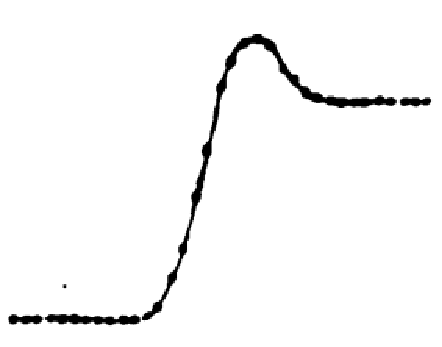
\includegraphics[width=\textwidth]{saccade_human_ori}
        \caption{}
        \label{fig:saccade_human_ori}
    \end{subfigure}
    \hfill
    \begin{subfigure}{0.2\textwidth}
        \centering
        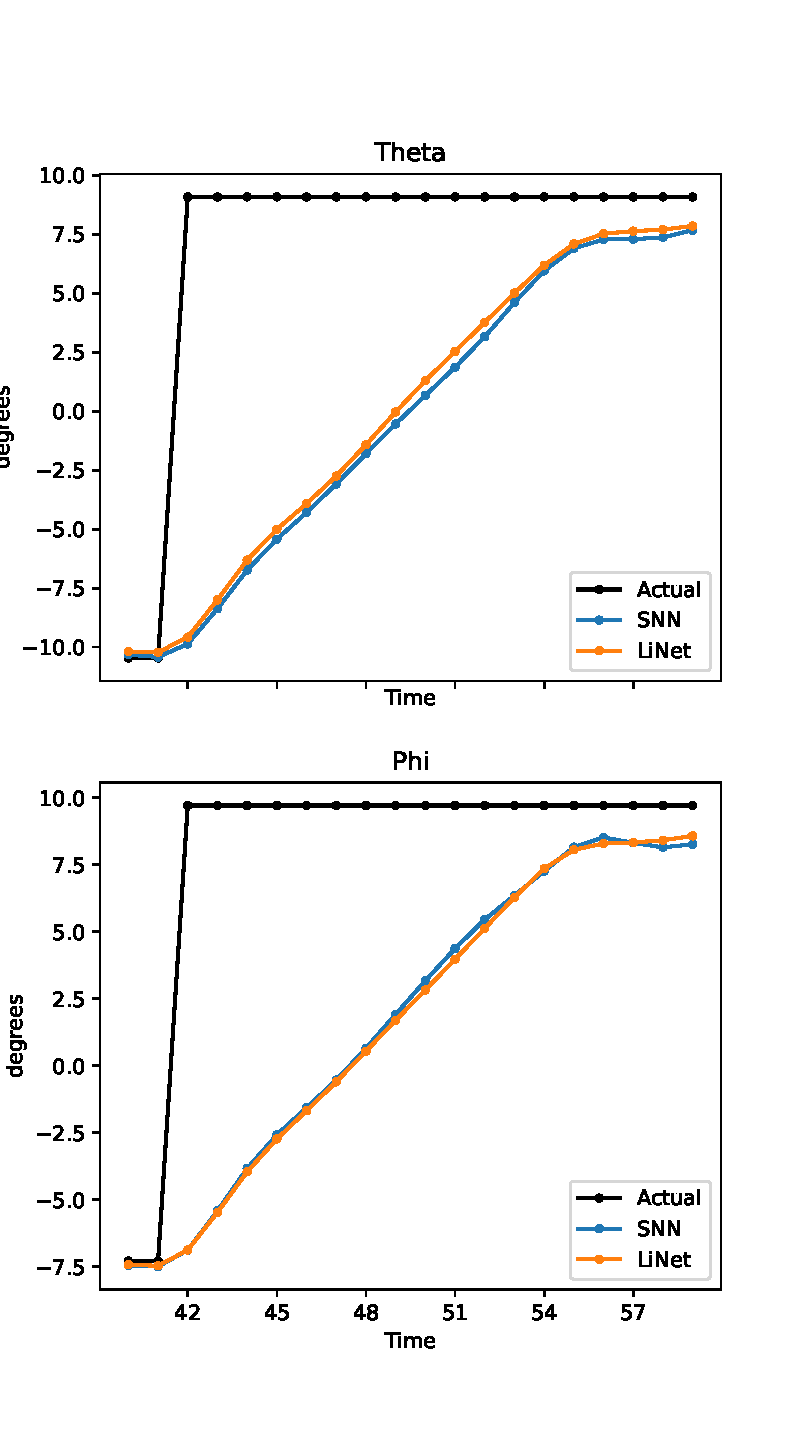
\includegraphics[width=\textwidth]{saccade_human_ori_normal}
        \caption{}
        \label{fig:saccade_human_ori_normal}
    \end{subfigure}
    \hfill
    \begin{subfigure}{0.2\textwidth}
        \centering
        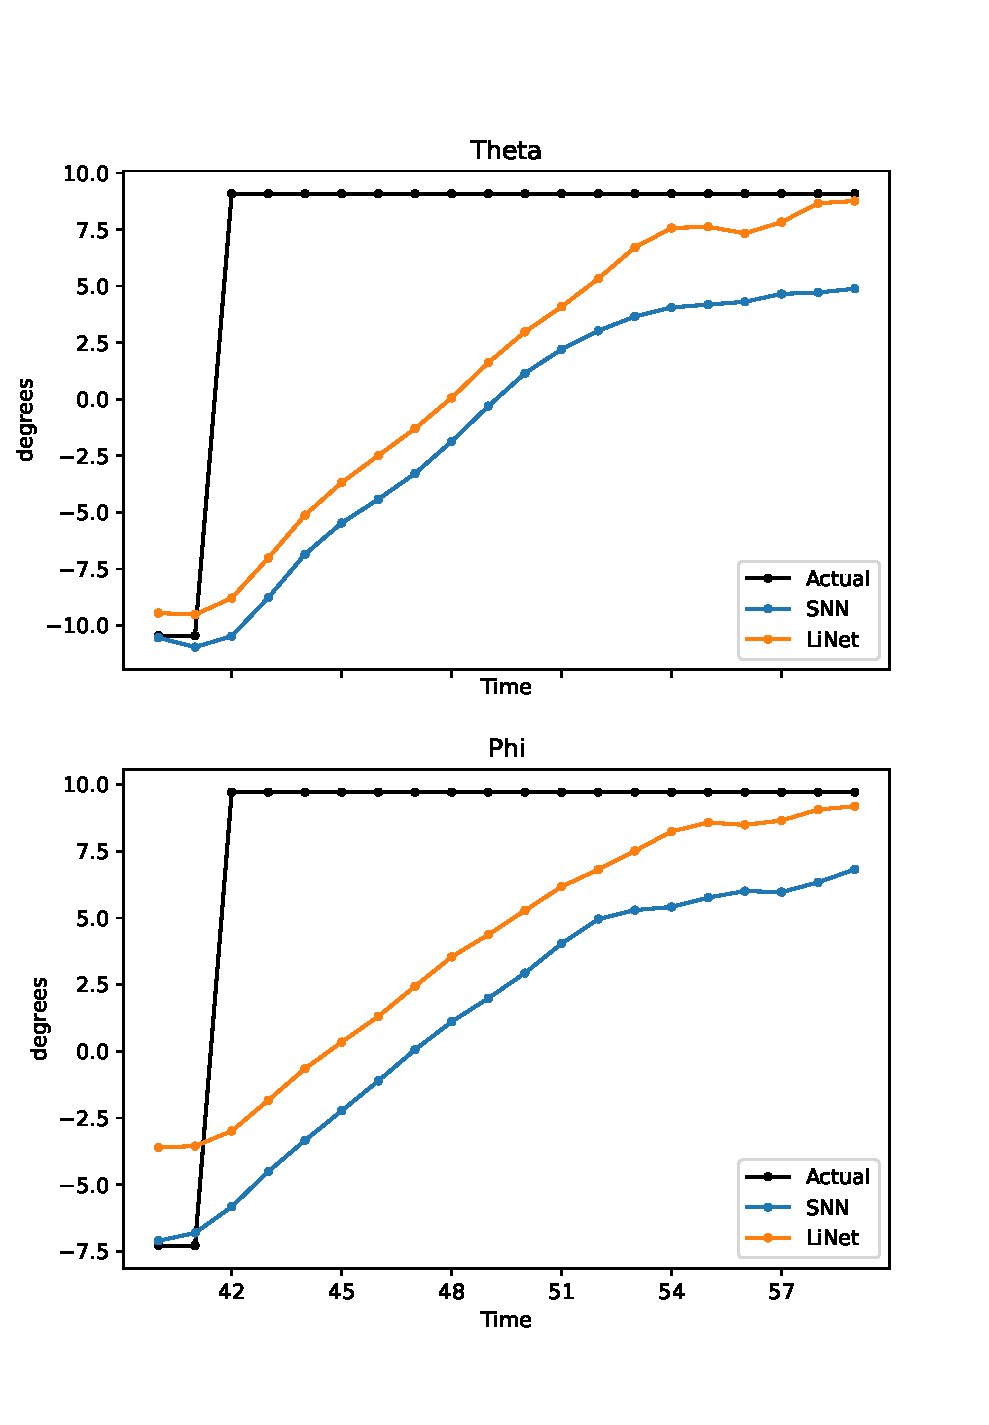
\includegraphics[width=\textwidth]{saccade_human_ori_delta}
        \caption{}
        \label{fig:saccade_human_ori_delta}
    \end{subfigure}

    \caption[Angular displacements from saccadic motion, compared to a human subject]{Comparison of angular displacements on saccadic motion. (a) Human. (b) ONV input. (c) D-ONV input.}
    \label{fig:saccade_ori}
\end{figure}

\begin{figure}
    \centering

    \begin{subfigure}{0.2\textwidth}
        \centering
        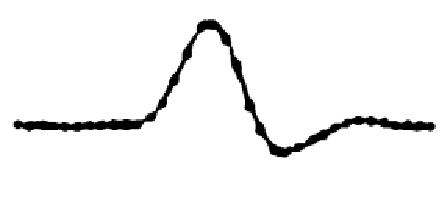
\includegraphics[width=\textwidth]{saccade_human_vel}
        \caption{}
        \label{fig:saccade_human_vel}
    \end{subfigure}
    \hfill
    \begin{subfigure}{0.2\textwidth}
        \centering
        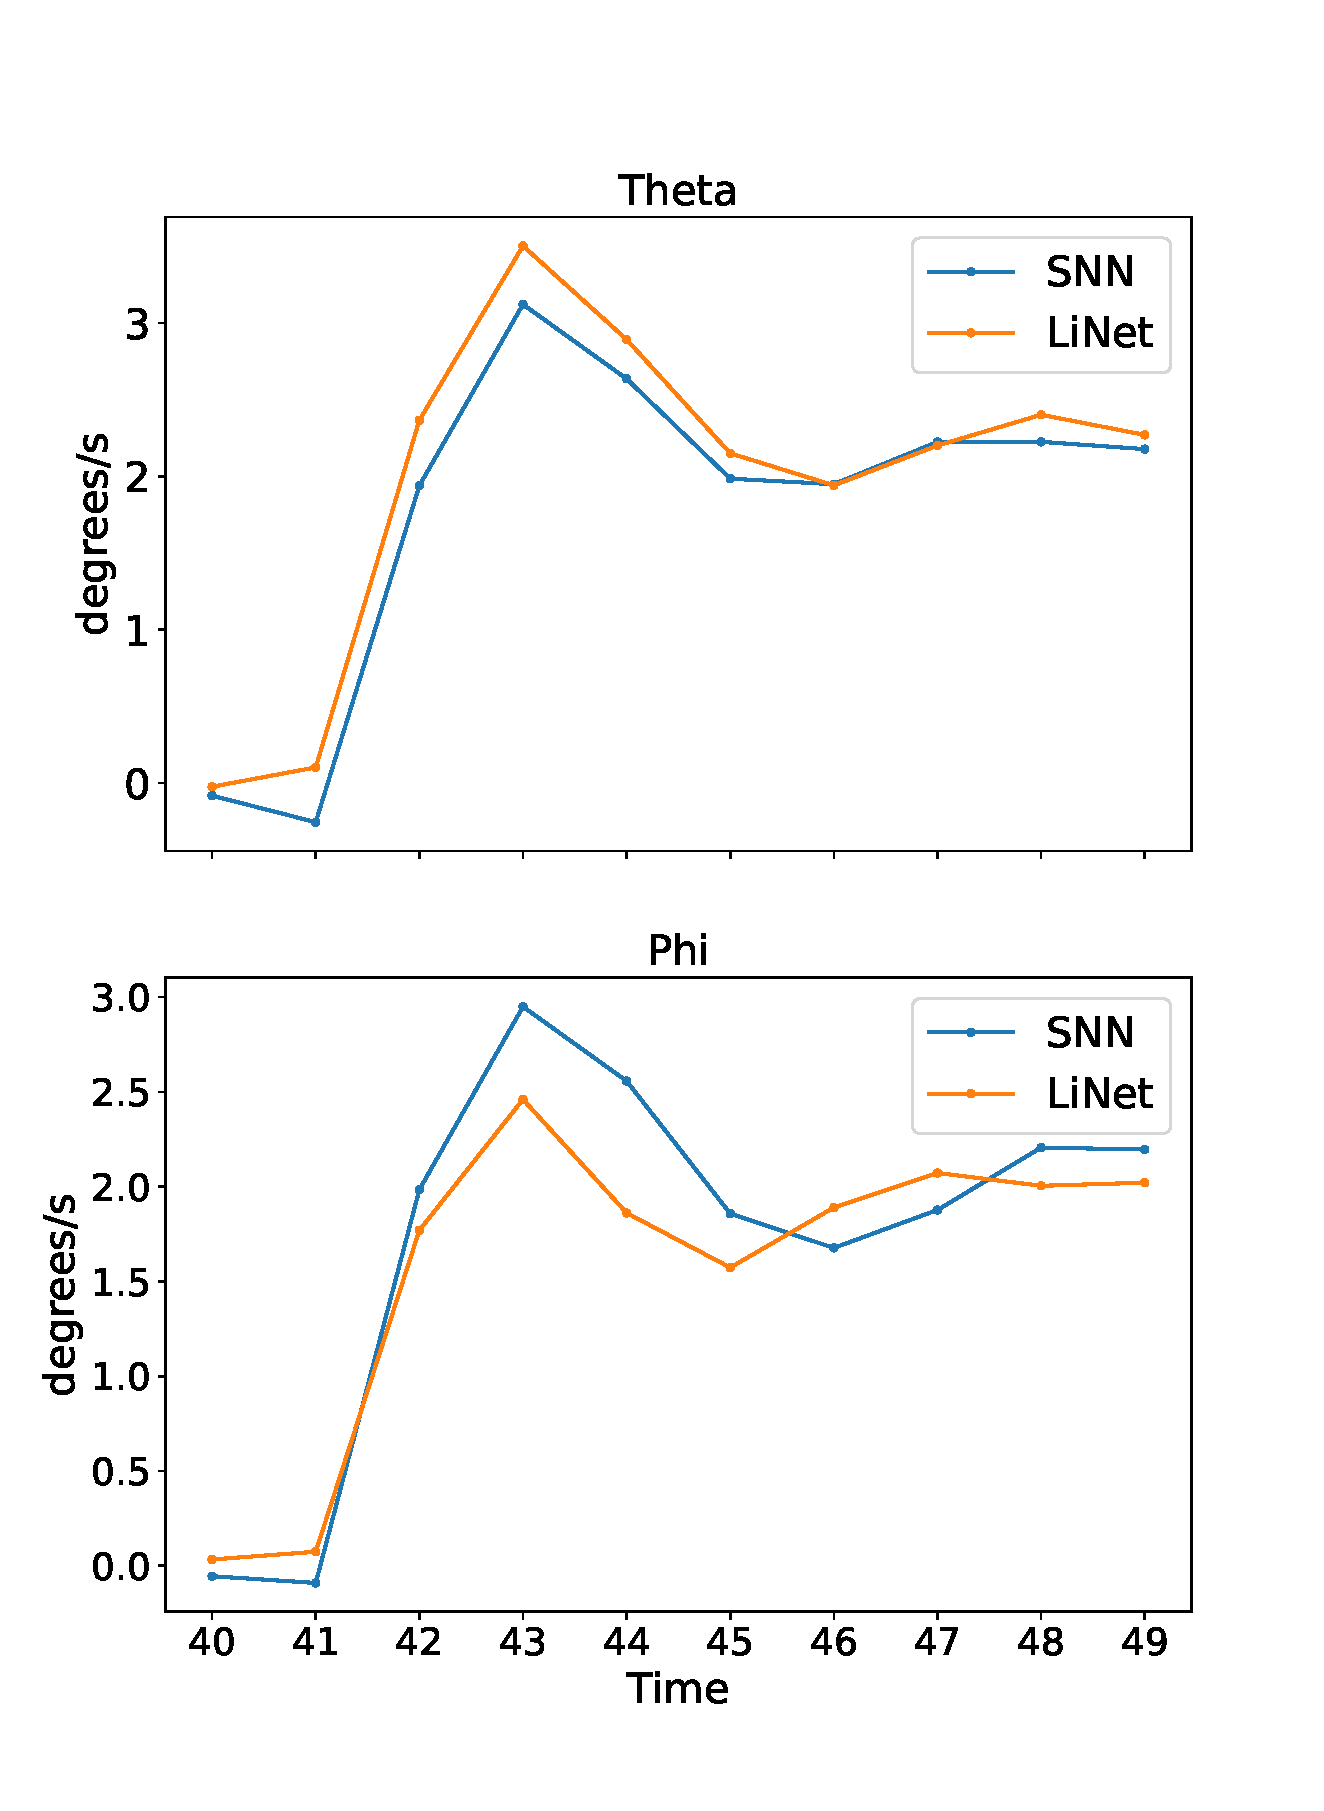
\includegraphics[width=\textwidth]{saccade_human_vel_normal}
        \caption{}
        \label{fig:saccade_human_vel_normal}
    \end{subfigure}
    \hfill
    \begin{subfigure}{0.2\textwidth}
        \centering
        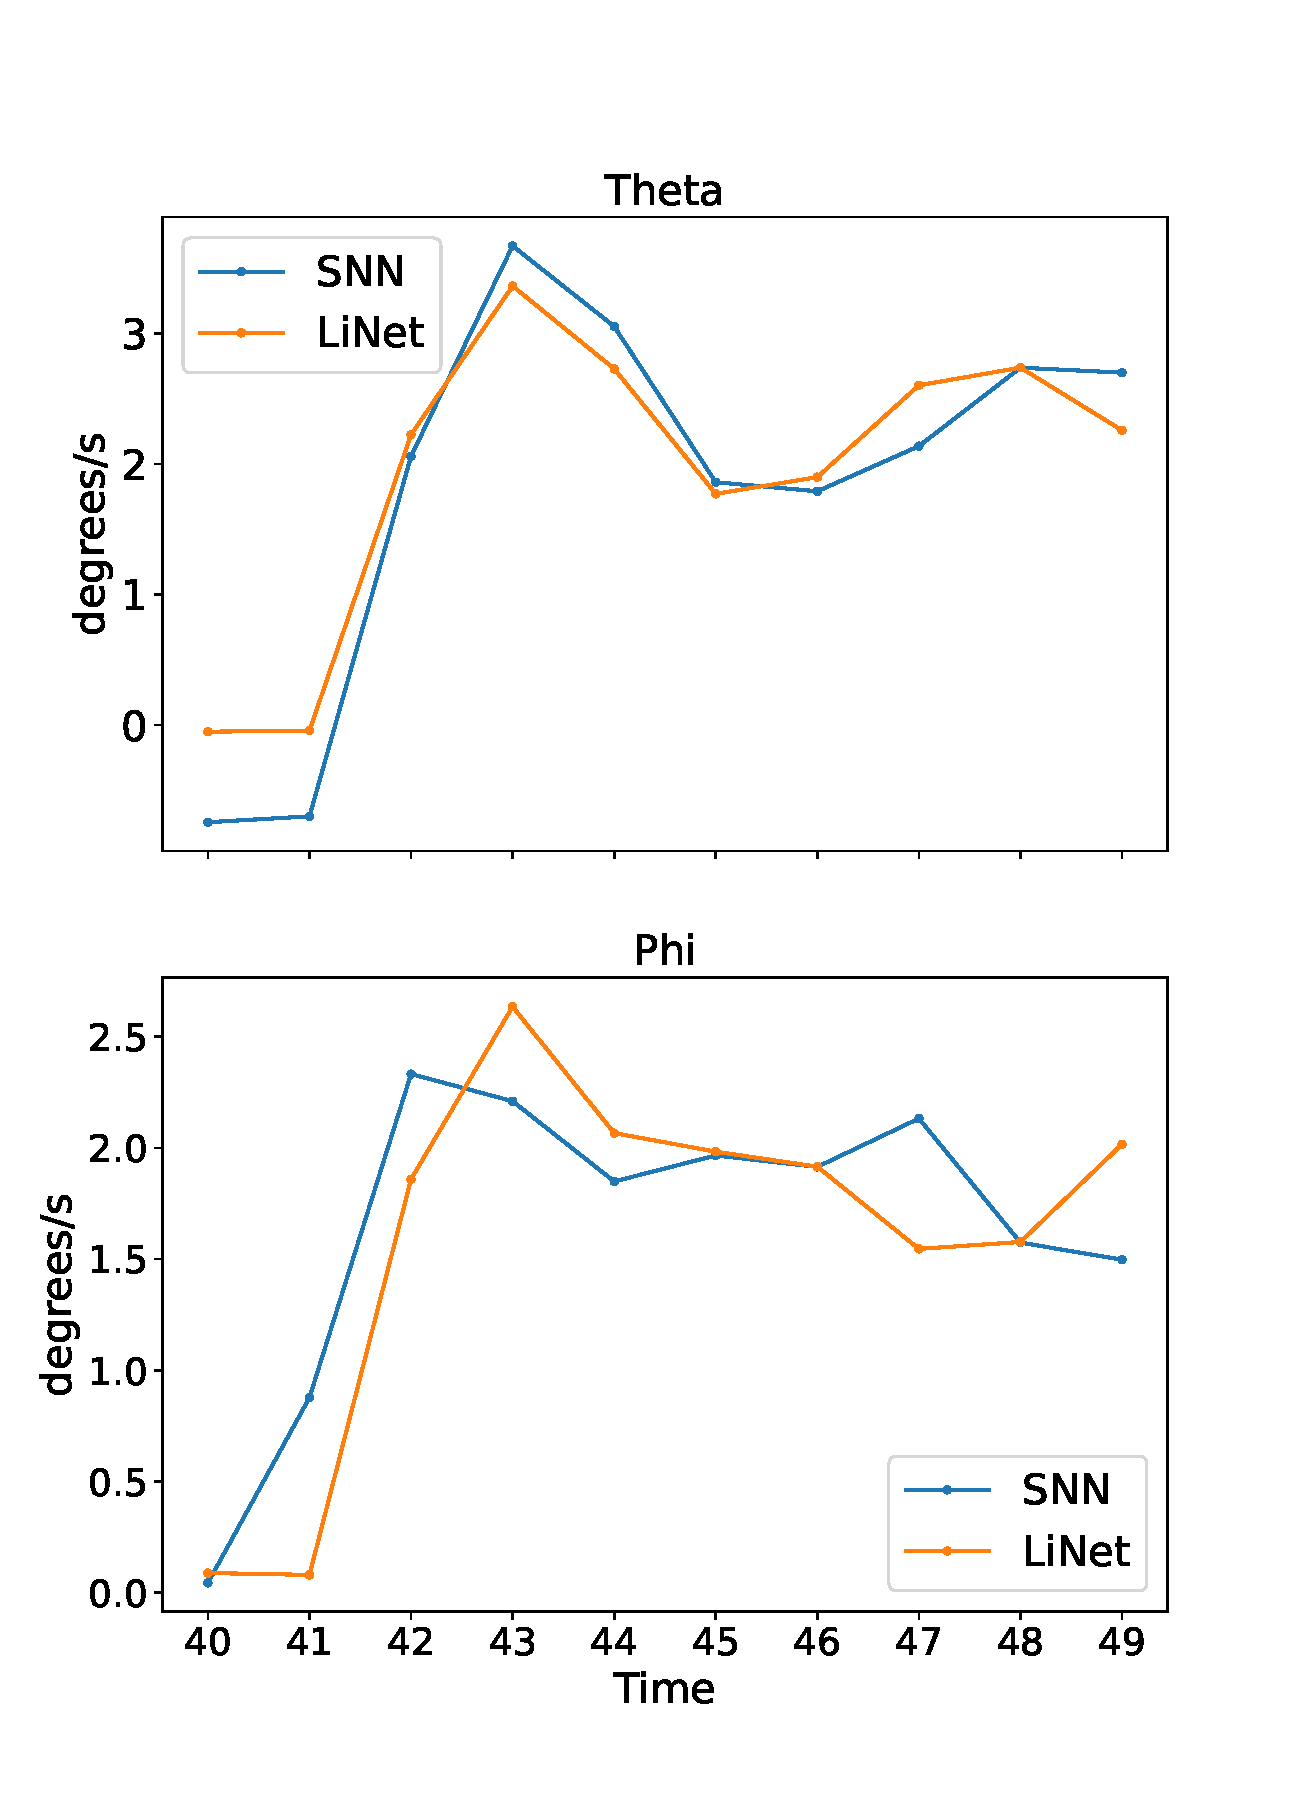
\includegraphics[width=\textwidth]{saccade_human_vel_delta}
        \caption{}
        \label{fig:saccade_human_vel_delta}
    \end{subfigure}

    \caption[Angular velocities from saccadic motion, compared to a human subject]{Comparison of angular velocities on saccadic motion. (a) Human. (b) ONV input. (c) D-ONV input.}
    \label{fig:saccade_vel}
\end{figure}

\begin{figure}
    \centering

    \begin{subfigure}{0.2\textwidth}
        \centering
        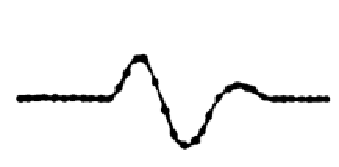
\includegraphics[width=\textwidth]{saccade_human_acc}
        \caption{}
        \label{fig:saccade_human_acc}
    \end{subfigure}
    \hfill
    \begin{subfigure}{0.2\textwidth}
        \centering
        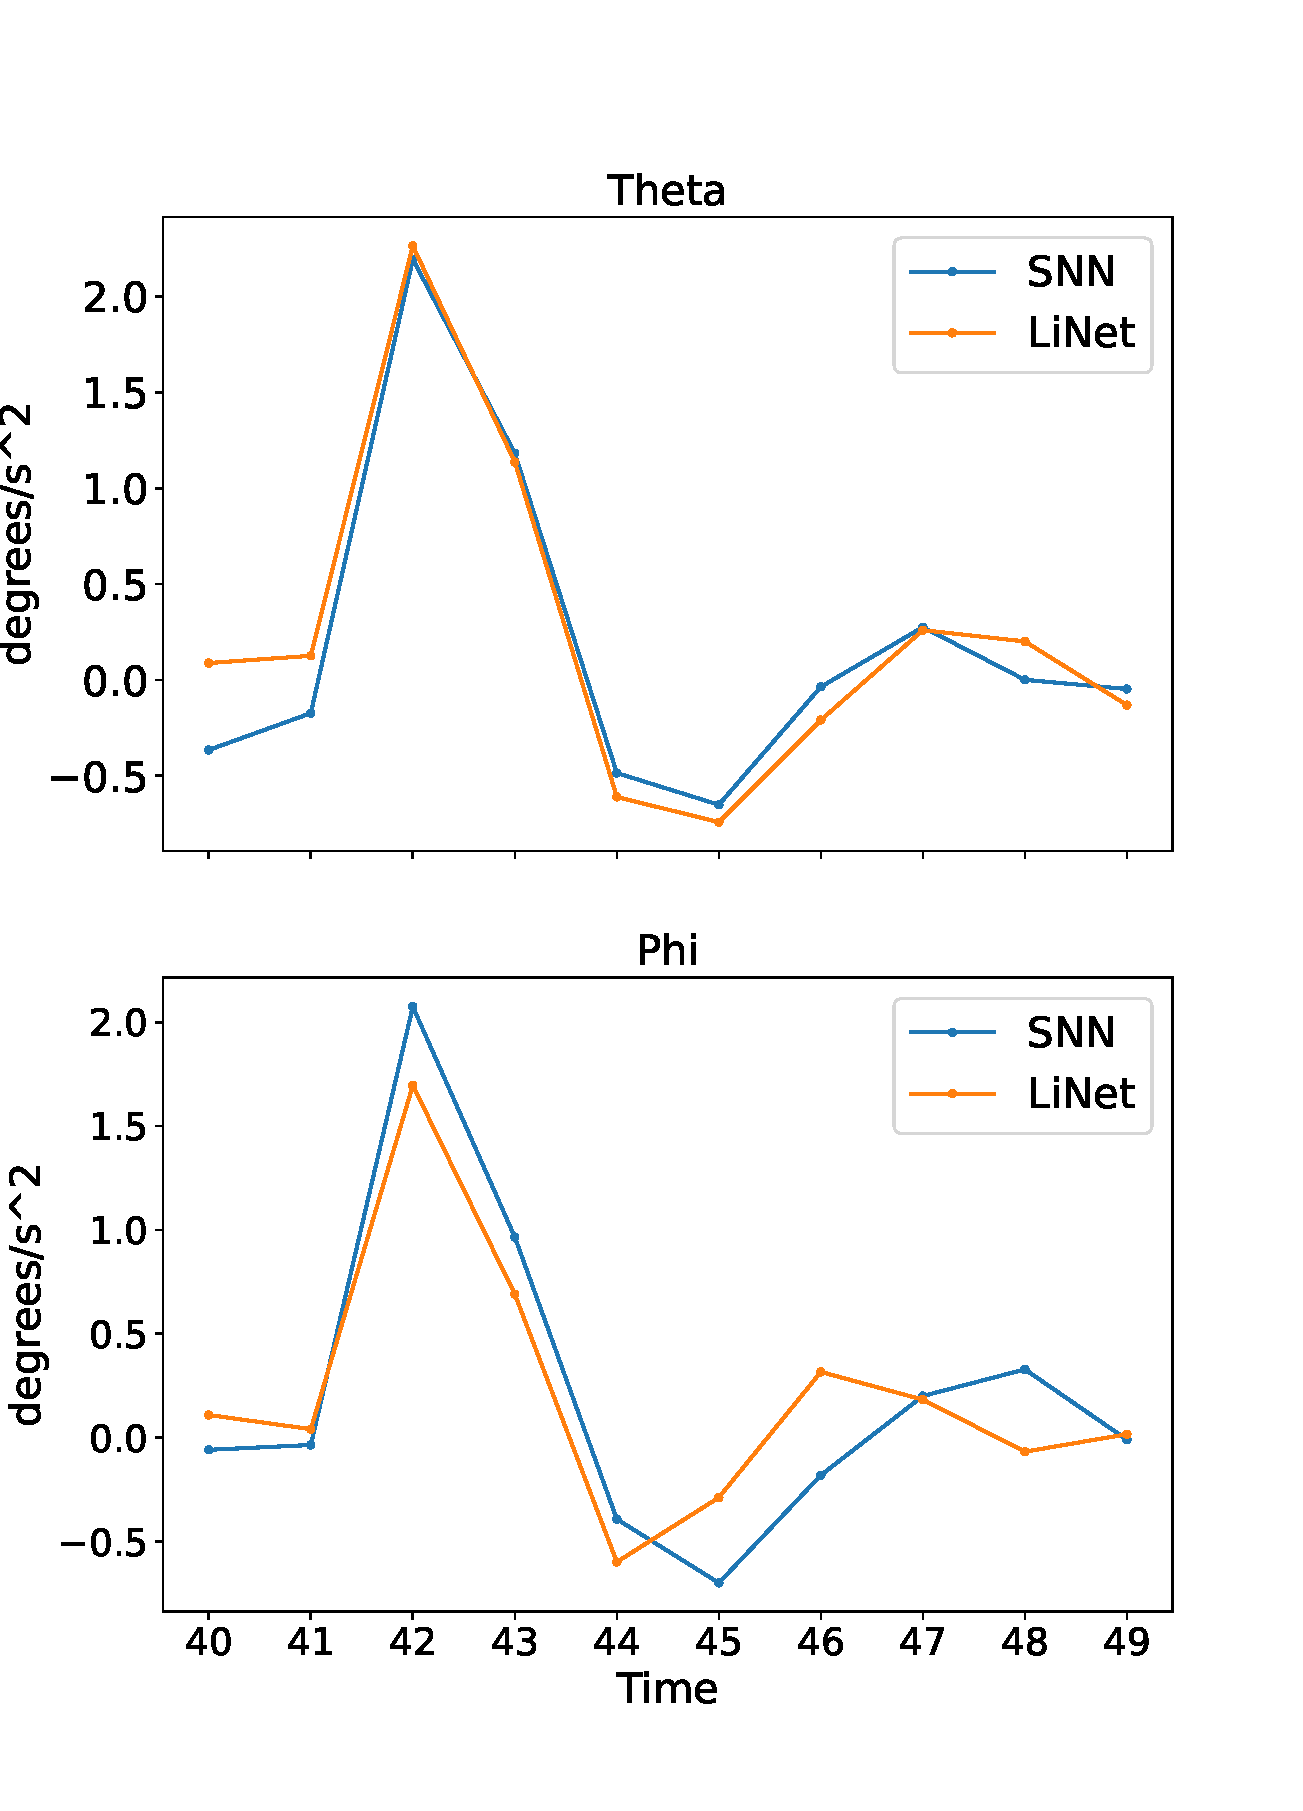
\includegraphics[width=\textwidth]{saccade_human_acc_normal}
        \caption{}
        \label{fig:saccade_human_acc_normal}
    \end{subfigure}
    \hfill
    \begin{subfigure}{0.2\textwidth}
        \centering
        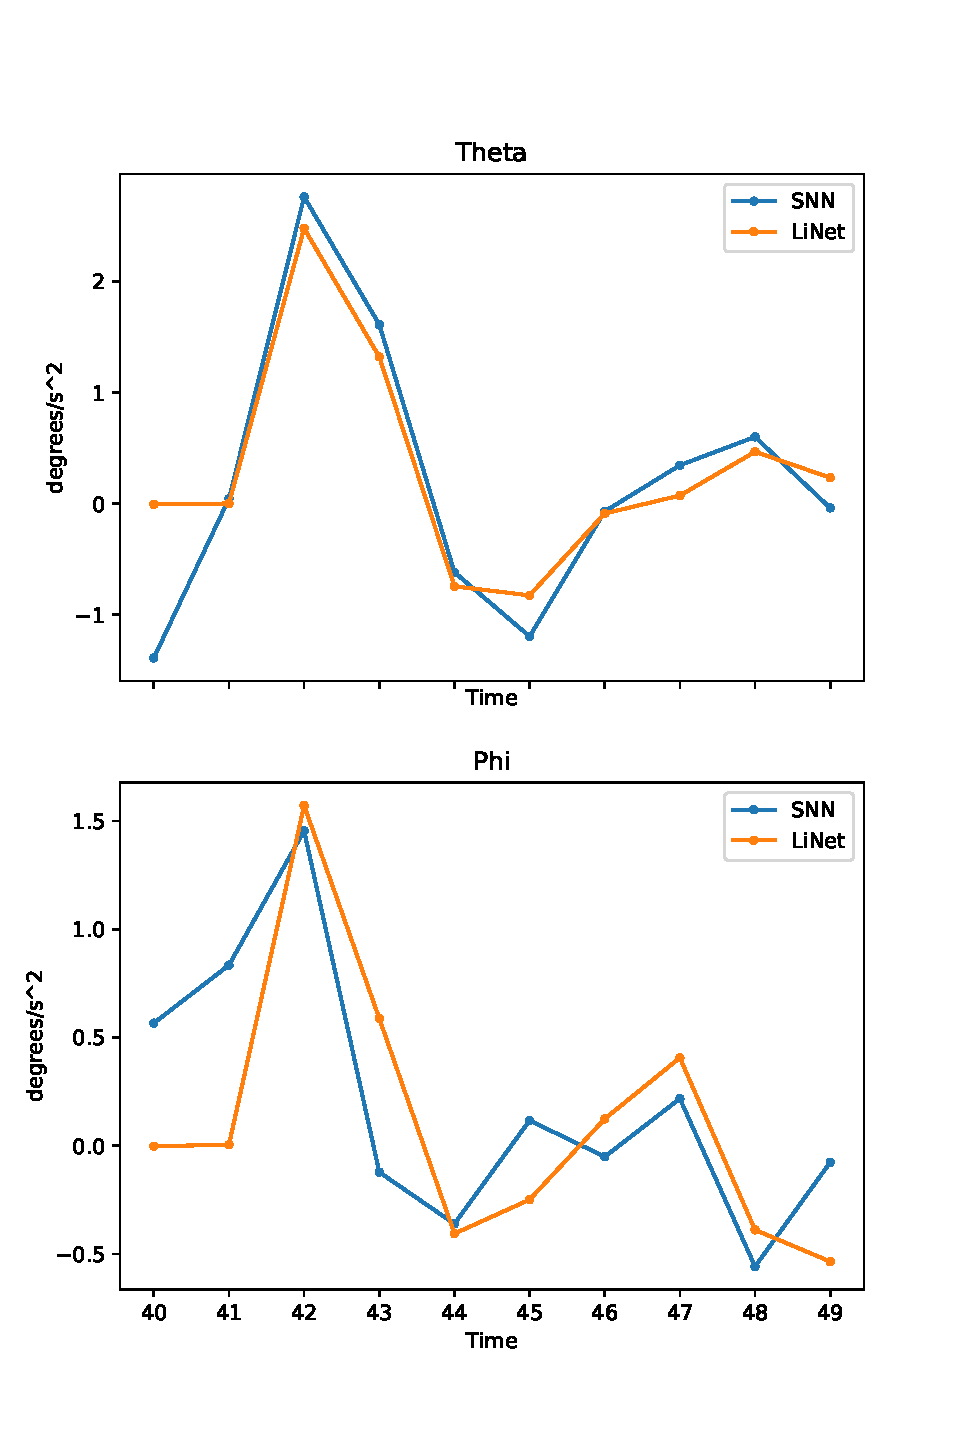
\includegraphics[width=\textwidth]{saccade_human_acc_delta}
        \caption{}
        \label{fig:saccade_human_acc_delta}
    \end{subfigure}

    \caption[Angular accelerations from saccadic motion, compared to a human subject]{Comparison of angular accelerations on saccadic motion. (a) Human. (b) ONV input. (c) D-ONV input.}
    \label{fig:saccade_acc}
\end{figure}

When comparing angular velocities in Figure~\ref{fig:saccade_vel} and angular accelerations in Figure~\ref{fig:saccade_acc}, we see that our SLiNet produces very similar curves to those of the human subject. The D-ONV traces deviate from the human traces slightly, but they have similar characteristics. However, the angular displacements in Figure~\ref{fig:saccade_ori} are not as close to that of the human subject. There is still a slight "bump" in all of the curves, but not as pronounced as we see in the human's. It is important to note that the human curves do not have reported amplitudes.

%********************************************************************%

% \section{Projectile Motion}

%********************************************************************%

\section{Spiking Analysis}

Unfortunately, we did not have access to neuromorphic hardware to validate the low-power benefit claims of SLiNets. Instead, we analyze the sparsity of computation in a SLiNet versus the LiNet. We look at the number of neurons in each layer that have a non-zero activation in the LiNet and the nuber of neurons that emit at least one spike in the SLiNet. 

% check tense for chapter two
Running our networks using the ONV examples from Figure~\ref{fig:onv_prev} and Figure~\ref{fig:onv_cur}, we see a similar amount of activated neurons in the LiNet and SLiNet. However, with the D-ONV from Figure~\ref{fig:onv_delta}, the SLiNet uses much fewer neurons in the first few layers, which contain most of them. We summarize these results in Table~\ref{table:onv_delta} and present the membrane voltages over time for a subset of neurons from the first layer of our SLiNet in Figure~\ref{fig:spike_traces}.

% look at thresholds, membranes, spike rates?

\begin{table}
    \centering
    \begin{tabular}{c c c c} 
        \toprule
        Layer & Number of Neurons & LiNet Activations (\%) & SLiNet Activations (\%)\\ 
        \midrule
        1 & 8,640 & 32 & 2.4 \\ 
        
        2 & 1,728 & 21 & 7 \\
        
        3 & 345 & 33 & 17 \\
        
        4 & 69 & 39 & 45 \\
        
        5 & 13 & 31 & - \\ 
        \bottomrule
    \end{tabular}
    \caption[Percentage of neurons activated in the LiNet vs the SLiNet]{Comparing the percentage of neurons activated in each layer of the LiNet and the SLiNet when using the ONV from Figure~\ref{fig:onv_delta} as input. An activated neuron in the LiNet outputs a non-zero value while an activated neuron in the SLiNet outputs at least one spike in the simulated time interval. There are significantly fewer activated neurons in the first few layers when using the SLiNet, thus demonstrating the sparse computation that results from using the D-ONV and spiking neurons.}
    \label{table:onv_delta}
\end{table}

%********************************************************************%

% compare membrane voltage graphs to actual retinal spikes?

\begin{figure}
    \centering
    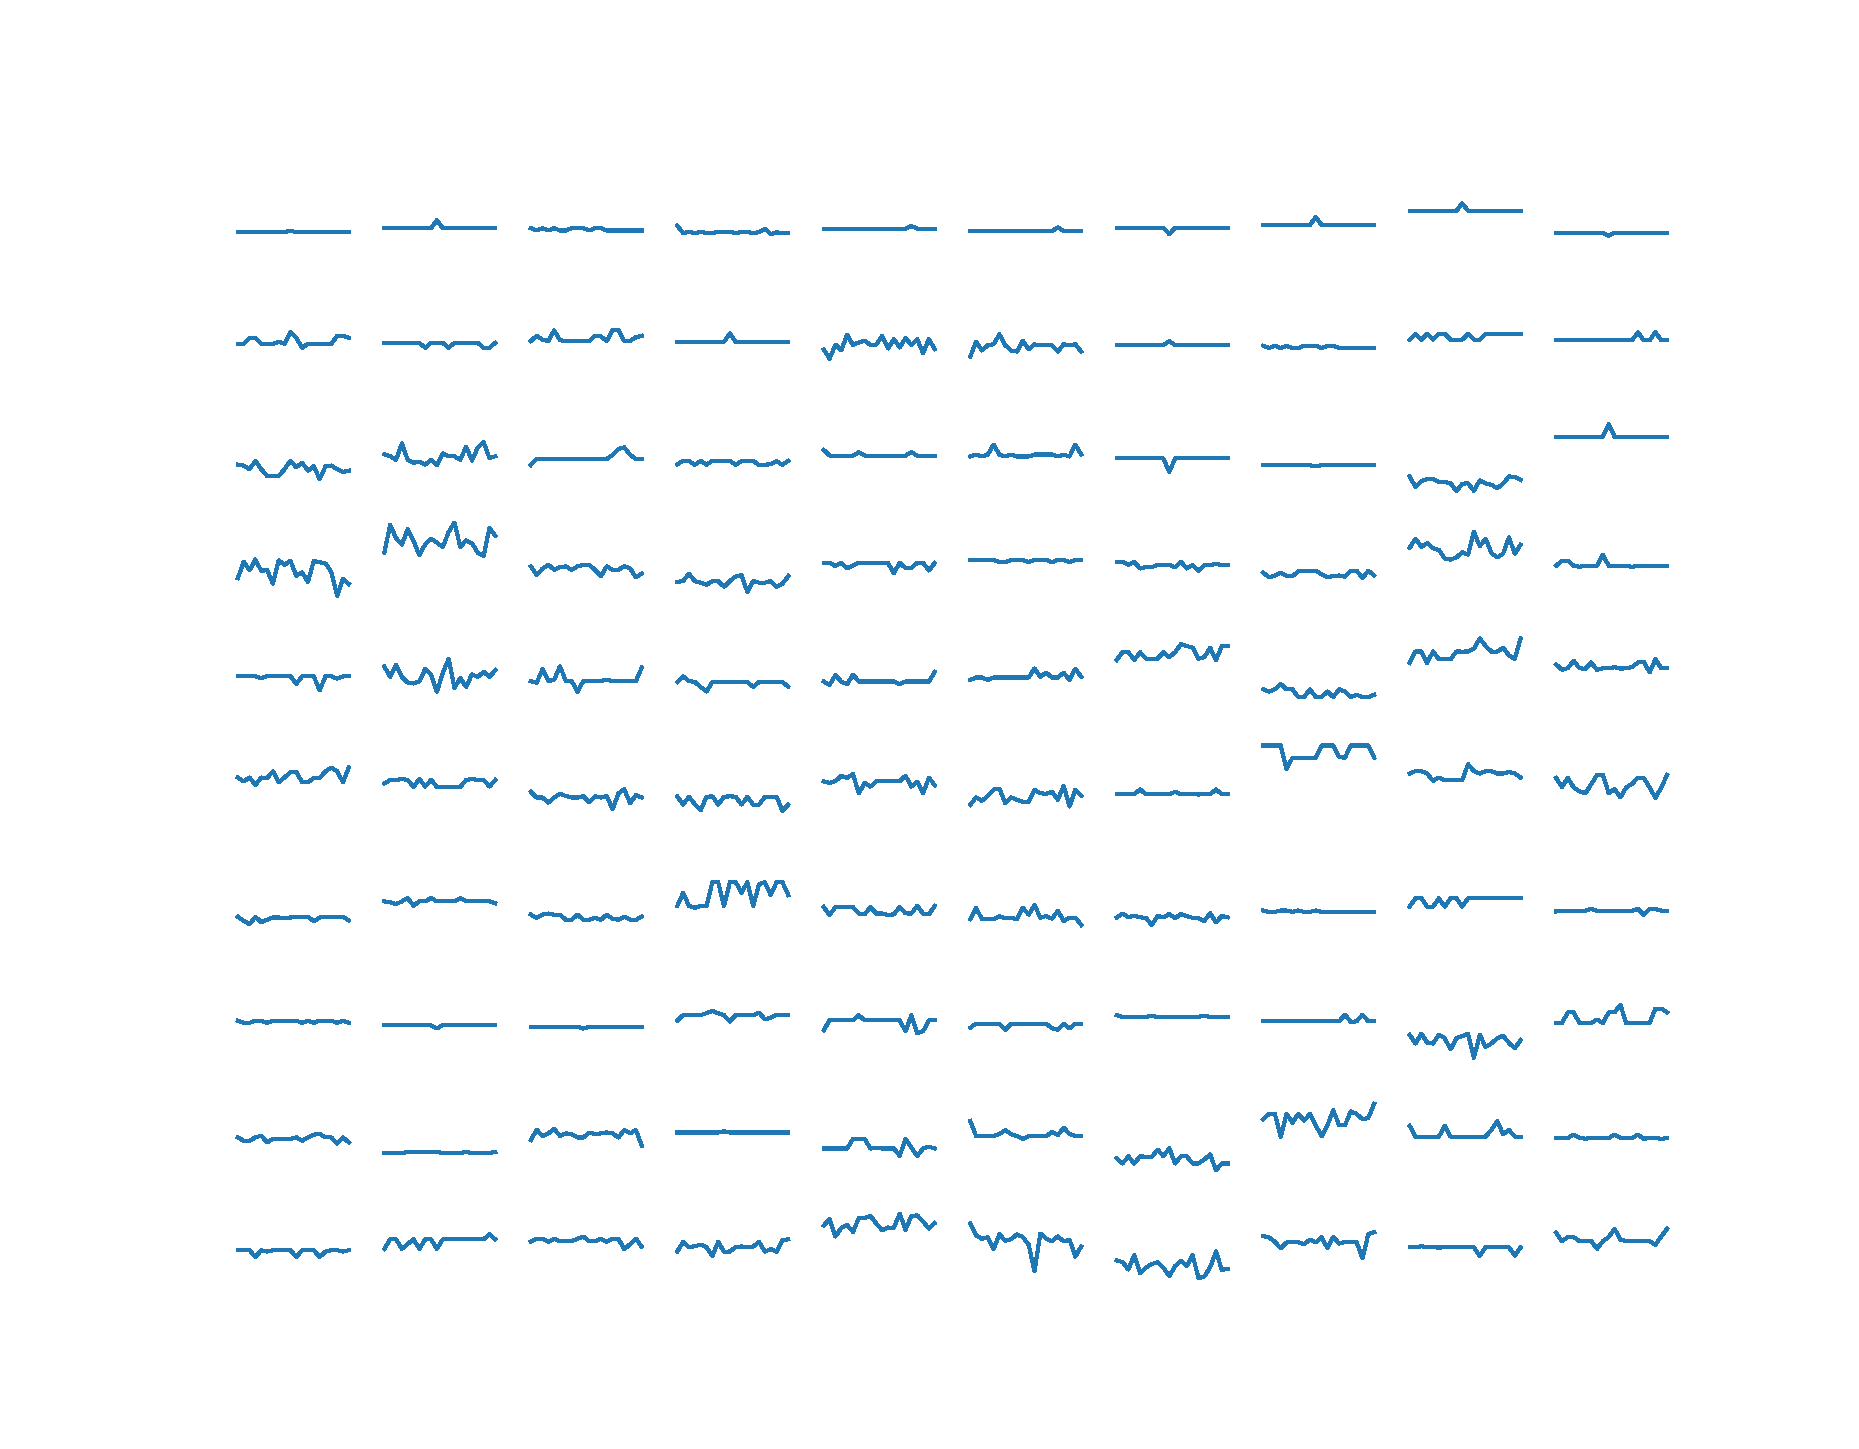
\includegraphics[width=1.0\textwidth]{spike_traces}
    \caption[Sample membrane voltage traces]{A plot of membrane voltages over time for a subset of 100 neurons from the first layer of our SLiNet, processing the ONV from Figure~\ref{fig:onv_delta}. We see consistent spiking patterns from certain neurons, similar to real neuron spike trains. Many neurons are also not excited and have relatively flat voltage traces.}
    \label{fig:spike_traces}
\end{figure}


%%%%%%%%%%%%%%%%%%%%%%%%%%%%%%%%%%%%%%%%%%%%%%%%%%%%%%%%%%%%%%%%%%%%%%

\chapter{Conclusion}

% first, second
This thesis has made two significant additions to the biomimetic eye model of \citet{Masaki, Arjun_thesis, Masaki_linet}. First, we replaced the foveation LiNet with a more biologically plausible spiking neural network (SNN). Second, we trained our SLiNet on event-based data, allowing the eye to detect changes in the scene when performing visual tracking. In addition, our spike encoding method emulates the processing done by neurons at the retinal level and allows for sparse computation when compared to traditional ANNs. Finally, backpropagation training an SNN from scratch to solve a regression task was a novel achievement. 

%********************************************************************%

\section{Discussion}

Across all of our tests, the SLiNet was successfully able to track the target when using either the ONV or the D-ONV. The LiNet did not perform well with the D-ONV as input. We note, however, that the use of a D-ONV with our SLiNet resulted in noisier eye movements. This makes sense intuitively, as small movements are utilized to generate events that the eye can process to confirm where the ball is. Without these micro-saccadic movements, there would be fewer input events and the eye would likely struggle to track the ball.

Our SLiNet did not perfectly match the training performance of the LiNet. The LiNet converges very quickly and achieves lower training and validation loss values. However, our SLiNet still converges to a usable state. The LiNet's relatively large validation loss was an indication that it would struggle while using the D-ONV.

% There is also the fact that we require neuromorphic hardware to become more mainstream to verify that the energy savings of our work make it an attractive option over a LiNet. 

Additionally, our SLiNet was able to run using a relatively low number of timesteps. This is likely tied to the use of a gain factor in our rate encoding scheme, which encourages more neurons to spike more frequently.

Training our SLiNet from scratch allows for the use of more natural spike encoding methods when compared to converted SNNs. However, we were not able to comapare our model's performance with that of a converted SNN. Nevertheless, we believe that our work lays the groundwork for exploring different learning mechanisms, which is more general than tuning network parameters for a specific task.


% It is interesting that the use of just one ReLU layer in the Hybrid SLiNet allows for very similar performance to that of a LiNet. Our SLiNet model still performs well but exhibits more side to side motions. The SLiNet model is great for biological plausibility, but the Hybrid SLiNet allows for more efficient inference with most of the advnatages of an SLiNet.

%********************************************************************%

\section{Future Work}

% replace other NNs with SNNs

Many learning techniques are being studied outside of standard backpropagation. This includes spike time dependent plasticity (STDP), which is inspired by a theory of how neurons in the brain reinforce certain pathways \citep{stdp}. More experimental network layers, such as neuron ensembles with inhibition \citep{nengo}, can also inspire more biologically plausible networks and help identify how certain parts of the visual cortex work.

We are also interested in exploring why latency encoding was unusable with our model. It potentially offers significant power savings over rate encoding and would be a valuable topic for future research.

Related to the biomechanical human musculoskeletal model of \citet{Masaki}, we would like to explore the results of using two SLiNet-controlled eyes. The ONV as it stands is still a rather gross approximation in binocular vision, since the nervous system splits input from each eye into left and right regions at the optic chiasm. Exploring new architectures to process the visual input in this manner may offer interesting solutions. 

Finally, all the SNNs in our work were emulated using GPU hardware. Given access to neuromorphic hardware, we would like to verify the power and latency improvements proposed by our hybrid SNNs. We would also like to verify if our output spike interpretation method scales to other regression problems.

% Given the difficulty of working with the unstructured ONV input, we would like to see if SNNs can be trained on classification tasks with this eye model. This would simulate reading and be an interesting experiment. Some work has been done on PI-MNSIT \citep{}. Furthermore, finding one architecture to do both object tracking and classification would be closer to simulating the visual system.

%%%%%%%%%%%%%%%%%%%%%%%%%%%%%%%%%%%%%%%%%%%%%%%%%%%%%%%%%%%%%%%%%%%%%%

\appendix

%%%%%%%%%%%%%%%%%%%%%%%%%%%%%%%%%%%%%%%%%%%%%%%%%%%%%%%%%%%%%%%%%%%%%%

\chapter{The Biomimetic Eye Model}
\label{appendix:eye}

In this appendix we provide more detail about the biomimetic eye model of \citet{Arjun}.

\section{Ocular Organs and Muscles}

Light enters the eye through the pupil, and the iris is the muscle that controls the amount of light that makes its way to the retina. The iris is controlled in the simulation by two muscles: the pupillary sphincter, which constricts the pupil, and the pupillary dilator, which opens up the pupil. The pupil constricts when there is a large amount of light and it dilates when there is a low amount. 

The cornea and lens serve to refract light to focus it onto the retina. Similar to the iris, the lens lengthens and shortens. The lens lengthens to focus on more distant objects and shortens to focus on closer objects. 

Three pairs of extraocular (EO) muscles work together to move the eyeball with 3 degrees of freedom. One pair controls horizontal movement, one pair controls vertical movement, and the last pair creates a twisting motion.

All the muscles are simulated as Hill-type models.

\section{Oculomotor Control System}

A diagram of the oculomotor control system is shown in Figure~\ref{fig:eye_controller_summary}.

\begin{figure}
    \centering
    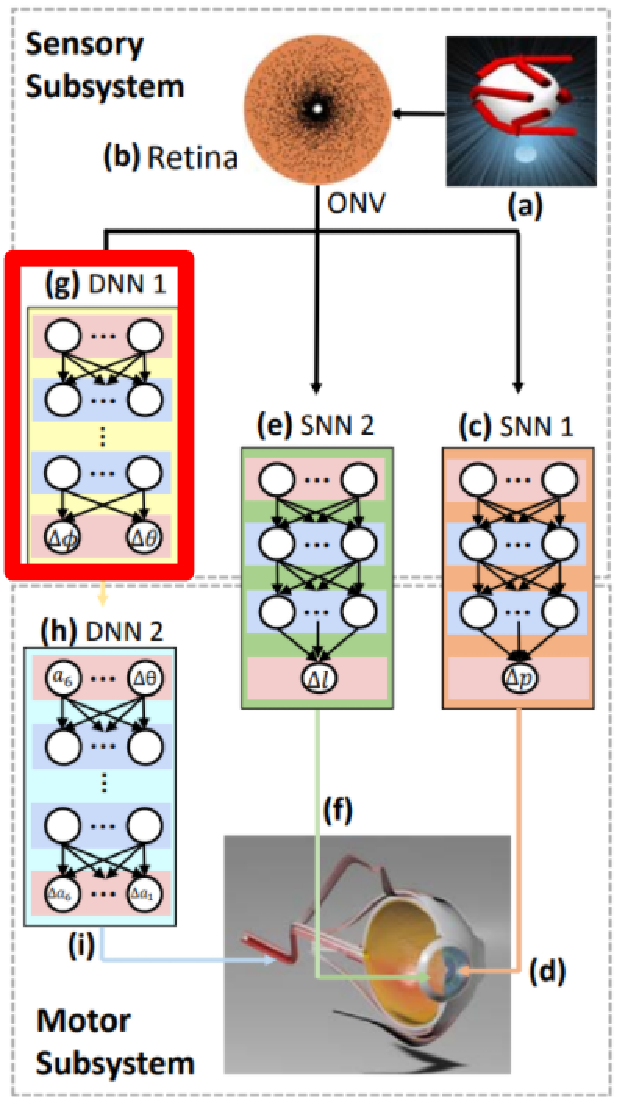
\includegraphics[width=0.5\textwidth]{subsystem_summary2}
    \caption[Diagram of the oculomotor control system]{Diagram of the eye's oculomotor control system. Note that SNN in this figure stands for ``shallow neural network'', not spiking neural network, and DNN stands for ``deep neural network.'' The system is comprised of a sensory subsystem (top) and a motor subsystem (bottom). Using ray-tracing (a), rays are cast from the positions of photoreceptors on the retina (b) into the 3D scene, from which a 43,200 dimensional ONV of photoreceptor responses is computed. SNN~1 (c) and SNN~2 (e) input the ONV and output pupil (d) and lens (f) muscle activations responsible for luminance and focal accommodation, respectively. The ONV is also input to the foveation DNN~1 (highlighted in red), which is implemented as a LiNet, and which we replace with an SNN in this thesis. It outputs gaze angle changes, $\Delta\theta$ and $\Delta\phi$, required to track a moving visual target under observation within the field of view. These are input to the neuromuscular DNN~2 (h), which outputs the activation signals that drive the EO muscles (i) to produce the required eye movement. Diagram adapted from \citep{Arjun}. }
    \label{fig:eye_controller_summary}
\end{figure}

\begin{figure}
    \centering
    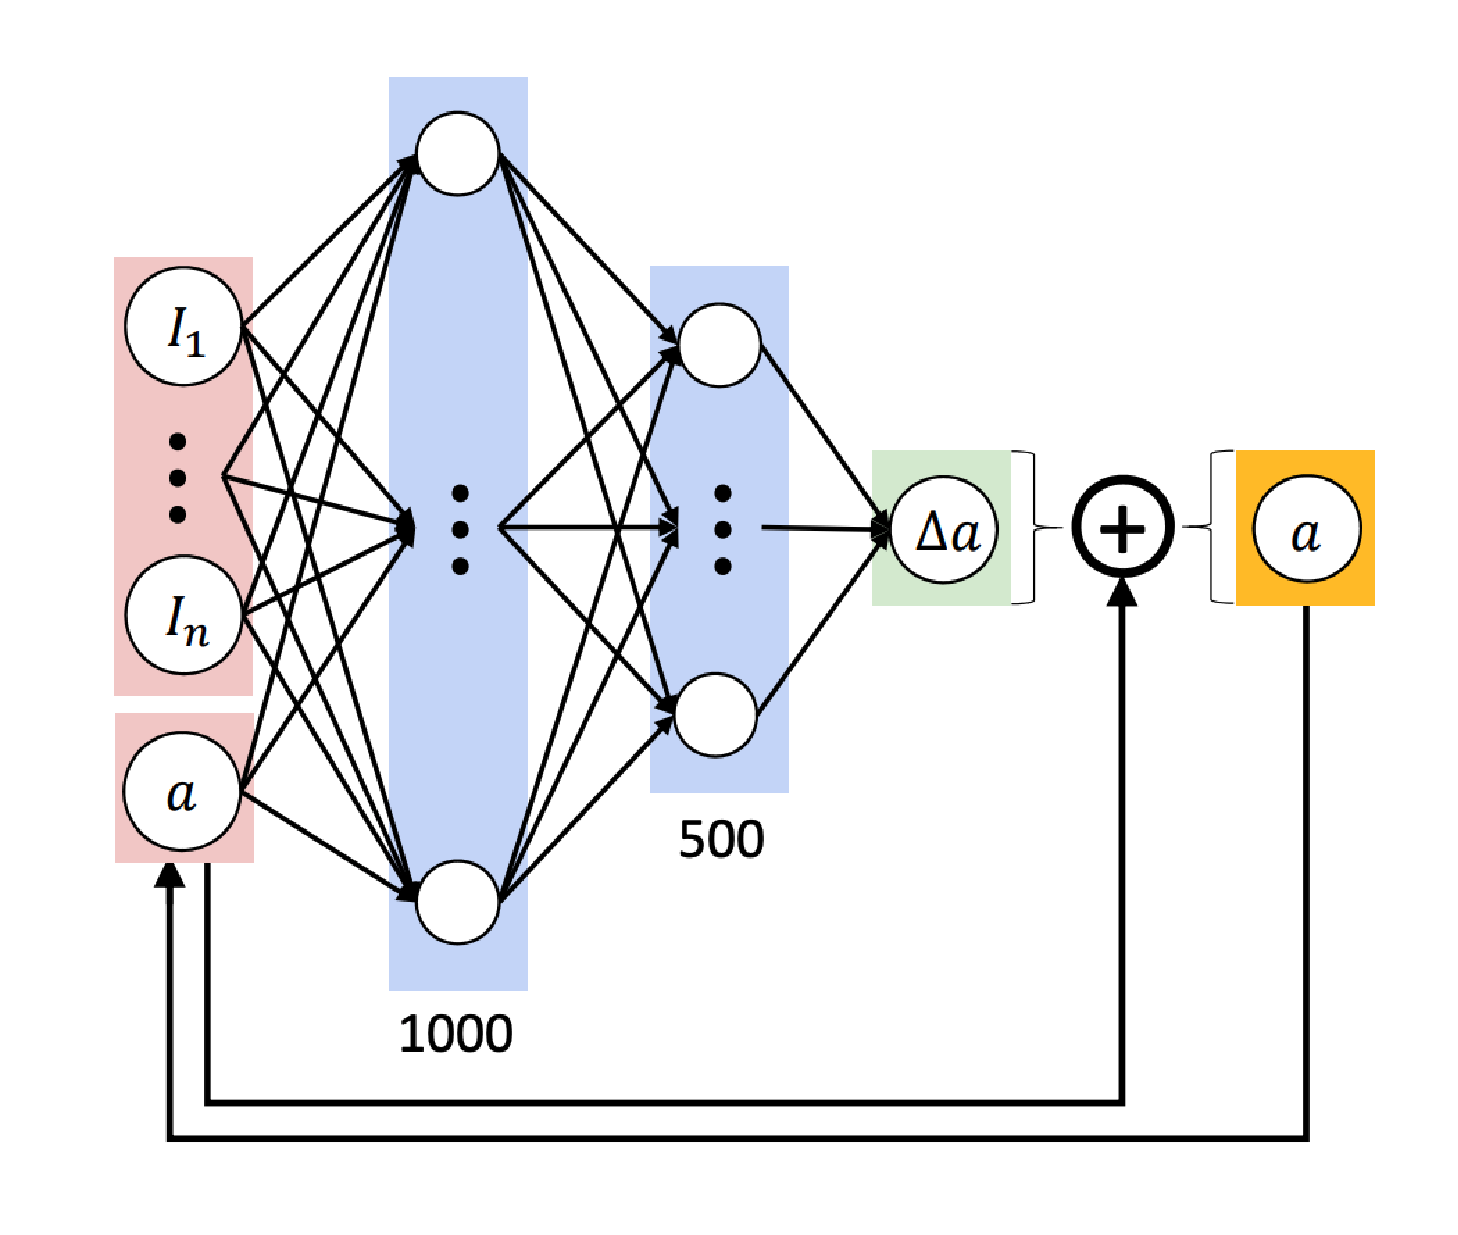
\includegraphics[width=0.5\textwidth]{controller_shallow}
    \caption[Shallow, fully connected pupil and lens controller]{The shallow, fully connected neural network architecture (labeled SNN~1 and SNN~2 in Figure~\ref{fig:eye_controller_summary}). Used to control the pupil and the lens. $I_1$ to $I_n$ represent the ONV intensities that are input to the network. A change in muscle activation is output, which is added to the current activation value and passed back as input for the next timestep. Due to this connection the network is recurrent. Diagram from \citep{Arjun}.}
    \label{fig:controller_shallow}
\end{figure}

\begin{figure}
    \centering
    \includegraphics[width=0.6\textwidth]{controller_deep}
    \caption[Deep, fully connected EO muscle controller]{The 6 layer, fully connected neural network used to control the EO muscles (labeled DNN~2 in Figure~\ref{fig:eye_controller_summary}). The current muscle activation values and angular displacement of the target are input to the network. Like the controller depicted in Figure~\ref{fig:controller_shallow}, this controller outputs changes in muscle activations and is recurrent. Diagram from \citep{Arjun}.}
    \label{fig:controller_deep}
\end{figure}

A single muscle activation signal dilates and constricts the pupil. This activation is provided by a shallow fully connected neural network whose architecture is shown in Figure~\ref{fig:controller_shallow}. Unlike the iris, the lens is modeled with damped springs. It uses the same shallow neural network architecture as the iris and uses one activation value to control lens curvature. The neural network that controls the EO muscles is a deep, fully connected network, shown in Figure~\ref{fig:controller_deep}. Like the other muscle controllers it outputs an activation value for each of the six muscles inducing them to contract. The neural networks are implemented as fully connected, recurrent models. Finally, the foveation DNN is illustrated in Figure~\ref{fig:linet_foveation}.

\begin{figure}
\centering
\includegraphics[width=\linewidth,trim={25mm 40mm 30mm 40mm},clip]{linet}
\caption{Foveation DNN architecture. A LiNet backbone is followed by a fully-connected layer that outputs $\Delta\theta$ and $\Delta\phi$. Diagram from \citep{Arjun}.}
\label{fig:linet_foveation}
\end{figure}


%%%%%%%%%%%%%%%%%%%%%%%%%%%%%%%%%%%%%%%%%%%%%%%%%%%%%%%%%%%%%%%%%%%%%%

\chapter{Mathematics of SNNs}
\label{appendix:snn}

To implement an SNN, we use snnTorch \citep{snnTorch}. The main way that SNNs differ from conventional ANNs is that the activation function only outputs either a 1 (a ``spike'') or a 0 (no spike) and that inputs vary over time. Neurons maintain an internal voltage that increases when their inputs spike and decays in the absence of input spikes. These changes allow SNNs to replace floating point multiplications with simple additions because synapse weights are only multiplied by 1's or 0's.

%********************************************************************%

\section{Circuit Model of a Spiking Neuron}
\label{sec:derivation}

\begin{figure}
    \centering
    \includegraphics[width=0.4\textwidth]{RC_neuron}
    \caption[RC circuit representation of a LIF neuron]{The RC circuit representation of a leaky integrate and fire neuron.}
    \label{fig:rc_circuit}
\end{figure}

The fundamental unit of an SNN is the leaky integrate-and-fire (LIF) neuron. It can be represented as an RC circuit, as shown in Figure~\ref{fig:rc_circuit}. From the circuit, using Kirchoff's current law, we obtain
\begin{equation}
    I_\text{in}(t) = I_R + I_C.
\end{equation}
Next, we derive equations for $ I_R $ and $ I_C $ by defining $V$, the voltage across the resistor, and $Q$, the charge on the capacitor. Using Ohm's law, $ I = V/R $, and the relationship $ Q = CU_\text{mem}(t) $, we write equations for the resistor,
\begin{equation}
    I_R(t) = \frac{U_\text{mem}(t)}{R},
\end{equation}
and the capacitor,
\begin{equation}
    I_C(t) = \frac{dQ}{dt} = C \frac{dU_\text{mem}(t)}{dt}.
\end{equation}
Placing these definitions into our original equation, we obtain
\begin{equation}
    I_\text{in}(t) = \frac{U_\text{mem}(t)}{R} + C \frac{dU_\text{mem}(t)}{dt}
\end{equation}
and
\begin{equation}
   RC \frac{dU_\text{mem}(t)}{dt} = -U_\text{mem}(t) + RI_\text{in}(t).  
\end{equation}
The units of the RHS are in voltage, while the term $\frac{dU_\text{mem}(t)}{dt}$ is in units of voltage/time. Therefore, the units of $RC$ must be in time, and we refer to this as the time constant $\tau$. This is a standard ordinary differential equation. Solving it analytically to determine that $ U_\text{mem}(t) = U_0 e ^{\frac{-t}{\tau}} $ would not be useful in a discrete-time neural network. Instead, starting from 
\begin{equation}
     \tau \frac{dU(t)}{dt} = -U(t) + RI_\text{in}(t),
\end{equation}
we use the definition of the derivative to write
\begin{equation}
    \tau \frac{U(t + \Delta t) - U(t)}{\Delta t}  \approx -U(t) + RI_\text{in}(t)
\end{equation}
and, ultimately, 
\begin{equation}
    U(t + \Delta t) \approx U(t) + \frac{\Delta t}{\tau} (-U(t) + RI_\text{in}(t)).
\end{equation}

% Insert graph of decaying membrane w/o input but increasing with input

With the above, we achieve the desired neuron model with a membrane potential that increases with input current and decays in the absence of any input. The equation involves many hyperparameters, which would be difficult to tune. Therefore, the snnTorch package simplifies the equation as follows:
\begin{equation}
   U(t + \Delta t) = (1 - \frac{\Delta t}{\tau}) U(t) + \frac{\Delta t}{\tau} R I_\text{in}(t).  
\end{equation}
We remove a term by assuming that $ I_\text{in}(t) = 0 $, as this input current will be replaced by the presynaptic inputs to the neuron, thus obtaining
\begin{equation}
     U(t + \Delta t) = (1 - \frac{\Delta t}{\tau}) U(t).
\end{equation}
Next, we denote the decay rate $(1 - \frac{\Delta t}{\tau}) = \beta$ (with $ \Delta t << \tau $ for reasonable accuracy) to write
\begin{equation}
    U(t + \Delta t) = \beta U(t).
\end{equation}

% skipped W derivation, not clear in tutorial
Because we want to work with discrete timesteps, we can assume $\Delta t = 1$. We also assume that $R=1$ in order to reduce the number of hyperparameters. Thus, we have the usable equation
\begin{equation}
   U(t+1) = \beta U(t) + W X(t+1), 
\end{equation}
where $W$ is a learnable parameter that weighs input spikes $X$. With $S(t)$ as our spiking function, we add a term to reset the membrane voltage when a neuron outputs a spike, and our final equation is
\begin{equation}
    U[t+1] = \underbrace{\beta U(t)}_{\text{decay}}
+ \underbrace{W X(t+1)}_{\text{input}}
- \underbrace{S(t)U_T}_{\text{reset}},
\end{equation}
with
\begin{equation}
    S[t] = \begin{cases} 
      1 & \text{if } U(t) > U_T, \\
      0 & \text{otherwise.}
      \end{cases}
\end{equation}

%********************************************************************%

\section{Loop Unroll}

From a computational graph perspective, SNNs are very similar to recurrent neural networks (RNNs), and we can use backpropagation through time (BPTT) to train our networks. The unrolled computation graph is shown in Figure~\ref{fig:snn_loop_unroll}.

\begin{figure}
    \centering
    \includegraphics[width=0.7\textwidth]{snnTorch_bptt}
    \caption[Unrolled computation graph for an SNN]{Computation graph for an SNN, similar to an RNN. $X(t)$ is the time-varying, spiking input. After multiplication by the weights, the spikes become input current to the neuron. The membrane voltage $U(t)$ and spiking activation $S(t)$ functions are derived in Section~\ref{sec:derivation}. Finally, the loss values $\mathcal{L}$ are computed at each timestep. Diagram from \citep{snnTorch}.}
    \label{fig:snn_loop_unroll}
\end{figure}

%********************************************************************%

\section{Neuron Parameters}

We detail more neuron design choices regarding the type of spiking neuron that we use in our work:

% WTA
Inhibition is an interesting option. In real neurons, the activation of one neuron can inhibit other neurons from firing. Our more traditional architecture would have very sparse spiking with this type of learning enabled, so we do not use it. However, spiking RNNs may benefit from this feature.

Neurons can be distinguished by what is known as their order. A second-order neuron accounts for the fact that when a presynaptic neuron fires, it takes time for the signal to reach the current neuron. This is accounted for by adding a second hyperparameter $\alpha$. These models are more complex to train and resulted in higher loss values, so we use first-order spiking neurons in  our work.

%%%%%%%%%%%%%%%%%%%%%%%%%%%%%%%%%%%%%%%%%%%%%%%%%%%%%%%%%%%%%%%%%%%%%%

\bibliographystyle {UCLAthesis}
\bibliography{thesis}

\end {document}